\documentclass[]{article}
\usepackage{lmodern}
\usepackage{amssymb,amsmath}
\usepackage{ifxetex,ifluatex}
\usepackage{fixltx2e} % provides \textsubscript
\ifnum 0\ifxetex 1\fi\ifluatex 1\fi=0 % if pdftex
  \usepackage[T1]{fontenc}
  \usepackage[utf8]{inputenc}
\else % if luatex or xelatex
  \ifxetex
    \usepackage{mathspec}
  \else
    \usepackage{fontspec}
  \fi
  \defaultfontfeatures{Ligatures=TeX,Scale=MatchLowercase}
\fi
% use upquote if available, for straight quotes in verbatim environments
\IfFileExists{upquote.sty}{\usepackage{upquote}}{}
% use microtype if available
\IfFileExists{microtype.sty}{%
\usepackage{microtype}
\UseMicrotypeSet[protrusion]{basicmath} % disable protrusion for tt fonts
}{}
\usepackage[margin=1in]{geometry}
\usepackage{hyperref}
\hypersetup{unicode=true,
            pdftitle={Package ``"proteoQ"''},
            pdfborder={0 0 0},
            breaklinks=true}
\urlstyle{same}  % don't use monospace font for urls
\usepackage{color}
\usepackage{fancyvrb}
\newcommand{\VerbBar}{|}
\newcommand{\VERB}{\Verb[commandchars=\\\{\}]}
\DefineVerbatimEnvironment{Highlighting}{Verbatim}{commandchars=\\\{\}}
% Add ',fontsize=\small' for more characters per line
\usepackage{framed}
\definecolor{shadecolor}{RGB}{248,248,248}
\newenvironment{Shaded}{\begin{snugshade}}{\end{snugshade}}
\newcommand{\AlertTok}[1]{\textcolor[rgb]{0.94,0.16,0.16}{#1}}
\newcommand{\AnnotationTok}[1]{\textcolor[rgb]{0.56,0.35,0.01}{\textbf{\textit{#1}}}}
\newcommand{\AttributeTok}[1]{\textcolor[rgb]{0.77,0.63,0.00}{#1}}
\newcommand{\BaseNTok}[1]{\textcolor[rgb]{0.00,0.00,0.81}{#1}}
\newcommand{\BuiltInTok}[1]{#1}
\newcommand{\CharTok}[1]{\textcolor[rgb]{0.31,0.60,0.02}{#1}}
\newcommand{\CommentTok}[1]{\textcolor[rgb]{0.56,0.35,0.01}{\textit{#1}}}
\newcommand{\CommentVarTok}[1]{\textcolor[rgb]{0.56,0.35,0.01}{\textbf{\textit{#1}}}}
\newcommand{\ConstantTok}[1]{\textcolor[rgb]{0.00,0.00,0.00}{#1}}
\newcommand{\ControlFlowTok}[1]{\textcolor[rgb]{0.13,0.29,0.53}{\textbf{#1}}}
\newcommand{\DataTypeTok}[1]{\textcolor[rgb]{0.13,0.29,0.53}{#1}}
\newcommand{\DecValTok}[1]{\textcolor[rgb]{0.00,0.00,0.81}{#1}}
\newcommand{\DocumentationTok}[1]{\textcolor[rgb]{0.56,0.35,0.01}{\textbf{\textit{#1}}}}
\newcommand{\ErrorTok}[1]{\textcolor[rgb]{0.64,0.00,0.00}{\textbf{#1}}}
\newcommand{\ExtensionTok}[1]{#1}
\newcommand{\FloatTok}[1]{\textcolor[rgb]{0.00,0.00,0.81}{#1}}
\newcommand{\FunctionTok}[1]{\textcolor[rgb]{0.00,0.00,0.00}{#1}}
\newcommand{\ImportTok}[1]{#1}
\newcommand{\InformationTok}[1]{\textcolor[rgb]{0.56,0.35,0.01}{\textbf{\textit{#1}}}}
\newcommand{\KeywordTok}[1]{\textcolor[rgb]{0.13,0.29,0.53}{\textbf{#1}}}
\newcommand{\NormalTok}[1]{#1}
\newcommand{\OperatorTok}[1]{\textcolor[rgb]{0.81,0.36,0.00}{\textbf{#1}}}
\newcommand{\OtherTok}[1]{\textcolor[rgb]{0.56,0.35,0.01}{#1}}
\newcommand{\PreprocessorTok}[1]{\textcolor[rgb]{0.56,0.35,0.01}{\textit{#1}}}
\newcommand{\RegionMarkerTok}[1]{#1}
\newcommand{\SpecialCharTok}[1]{\textcolor[rgb]{0.00,0.00,0.00}{#1}}
\newcommand{\SpecialStringTok}[1]{\textcolor[rgb]{0.31,0.60,0.02}{#1}}
\newcommand{\StringTok}[1]{\textcolor[rgb]{0.31,0.60,0.02}{#1}}
\newcommand{\VariableTok}[1]{\textcolor[rgb]{0.00,0.00,0.00}{#1}}
\newcommand{\VerbatimStringTok}[1]{\textcolor[rgb]{0.31,0.60,0.02}{#1}}
\newcommand{\WarningTok}[1]{\textcolor[rgb]{0.56,0.35,0.01}{\textbf{\textit{#1}}}}
\usepackage{graphicx,grffile}
\makeatletter
\def\maxwidth{\ifdim\Gin@nat@width>\linewidth\linewidth\else\Gin@nat@width\fi}
\def\maxheight{\ifdim\Gin@nat@height>\textheight\textheight\else\Gin@nat@height\fi}
\makeatother
% Scale images if necessary, so that they will not overflow the page
% margins by default, and it is still possible to overwrite the defaults
% using explicit options in \includegraphics[width, height, ...]{}
\setkeys{Gin}{width=\maxwidth,height=\maxheight,keepaspectratio}
\IfFileExists{parskip.sty}{%
\usepackage{parskip}
}{% else
\setlength{\parindent}{0pt}
\setlength{\parskip}{6pt plus 2pt minus 1pt}
}
\setlength{\emergencystretch}{3em}  % prevent overfull lines
\providecommand{\tightlist}{%
  \setlength{\itemsep}{0pt}\setlength{\parskip}{0pt}}
\setcounter{secnumdepth}{0}
% Redefines (sub)paragraphs to behave more like sections
\ifx\paragraph\undefined\else
\let\oldparagraph\paragraph
\renewcommand{\paragraph}[1]{\oldparagraph{#1}\mbox{}}
\fi
\ifx\subparagraph\undefined\else
\let\oldsubparagraph\subparagraph
\renewcommand{\subparagraph}[1]{\oldsubparagraph{#1}\mbox{}}
\fi

%%% Use protect on footnotes to avoid problems with footnotes in titles
\let\rmarkdownfootnote\footnote%
\def\footnote{\protect\rmarkdownfootnote}

%%% Change title format to be more compact
\usepackage{titling}

% Create subtitle command for use in maketitle
\providecommand{\subtitle}[1]{
  \posttitle{
    \begin{center}\large#1\end{center}
    }
}

\setlength{\droptitle}{-2em}

  \title{Package ``"proteoQ"''}
    \pretitle{\vspace{\droptitle}\centering\huge}
  \posttitle{\par}
    \author{}
    \preauthor{}\postauthor{}
      \predate{\centering\large\emph}
  \postdate{\par}
    \date{2019-06-14}


\begin{document}
\maketitle

{
\setcounter{tocdepth}{2}
\tableofcontents
}
\hypertarget{introduction-to-proteoq}{%
\subsection{Introduction to proteoQ}\label{introduction-to-proteoq}}

Chemical labeling using tandem mass tag
(\href{https://en.wikipedia.org/wiki/Tandem_mass_tag}{TMT}) has been
commonly applied in mass spectrometry (MS)-based quantification of
proteins and peptides. The \texttt{proteoQ} tool is designed to aid
automated and reproducible analysis of proteomics data. It interacts
with an \texttt{Excel} spread sheet for dynamic sample selections,
aesthetics controls and statistical modelings. The arrangement allows
users to put data manipulation behind the scene and apply metadata to
openly address biological questions using various informatic tools. In
addition, the entire workflow is documented and can be conveniently
reproduced upon revisiting.

The tool currently processes the peptide spectrum matches (PSM) tables
from \href{https://http://www.matrixscience.com/}{Mascot} searches for
6-, 10- or 11-plex TMT experiments. Peptide and protein results are then
produced with users' selection of parameters in data filtration,
alignment and normalization. The package further offers a suite of tools
and functionalities in statistics, informatics and data visualization by
creating `wrappers' around published R routines.

\hypertarget{installation}{%
\subsection{Installation}\label{installation}}

To install this package, start R (version ``3.6'') and enter:

\begin{Shaded}
\begin{Highlighting}[]
\ControlFlowTok{if}\NormalTok{ (}\OperatorTok{!}\KeywordTok{requireNamespace}\NormalTok{(}\StringTok{"BiocManager"}\NormalTok{, }\DataTypeTok{quietly =} \OtherTok{TRUE}\NormalTok{))}
    \KeywordTok{install.packages}\NormalTok{(}\StringTok{"BiocManager"}\NormalTok{)}
\NormalTok{BiocManager}\OperatorTok{::}\KeywordTok{install}\NormalTok{(}\KeywordTok{c}\NormalTok{(}\StringTok{"Biobase"}\NormalTok{, }\StringTok{"GSVA"}\NormalTok{, }\StringTok{"Mfuzz"}\NormalTok{, }\StringTok{"limma"}\NormalTok{))}

\ControlFlowTok{if}\NormalTok{ (}\OperatorTok{!}\KeywordTok{requireNamespace}\NormalTok{(}\StringTok{"devtools"}\NormalTok{, }\DataTypeTok{quietly =} \OtherTok{TRUE}\NormalTok{))}
    \KeywordTok{install.packages}\NormalTok{(}\StringTok{"devtools"}\NormalTok{)}
\NormalTok{devtools}\OperatorTok{::}\KeywordTok{install_github}\NormalTok{(}\StringTok{"qzhang503/proteoQ"}\NormalTok{)}
\end{Highlighting}
\end{Shaded}

\hypertarget{application-part-i}{%
\subsection{Application -- Part I}\label{application-part-i}}

In this section I illustrate the following applications of
\texttt{proteoQ}:

\begin{itemize}
\tightlist
\item
  Summarization of PSM data to peptide and protein reports.
\item
  Visualization of quality metrics in peptide and protein data.
\item
  Parital or complete re-normalization of data when needed
\end{itemize}

The data set I use in this section corresponds to the proteomics data
from Mertins et al.(2018). In the study, two different breast cancer
subtypes, triple negative (WHIM2) and luminal (WHIM16), from
patient-derived xenograft (PDX) models were assessed by three
independent laboratories. At each site, lysates from WHIM2 and WHIM16
were each split and labeled with 10-plex TMT at equal sample sizes and
repeated on a different day. This results in a total of 60 samples
labeled under six 10-plex TMT experiments. The samples under each
10-plex TMT were fractionated by off-line Hp-RP chromatography(2011),
followed by \texttt{LC/MS} analysis. The raw PSM results from
\href{https://http://www.matrixscience.com/}{Mascot} searches are stored
in a companion R package, \texttt{proteoQDA} and are accessbile through
the following installation:

\begin{Shaded}
\begin{Highlighting}[]
\NormalTok{devtools}\OperatorTok{::}\KeywordTok{install_github}\NormalTok{(}\StringTok{"qzhang503/proteoQDA"}\NormalTok{)}
\end{Highlighting}
\end{Shaded}

\hypertarget{set-up-the-experiments}{%
\subsubsection{Set up the experiments}\label{set-up-the-experiments}}

We first set up a working directory:

\begin{Shaded}
\begin{Highlighting}[]
\NormalTok{dat_dir <-}\StringTok{ "c:}\CharTok{\textbackslash{}\textbackslash{}}\StringTok{The}\CharTok{\textbackslash{}\textbackslash{}}\StringTok{First}\CharTok{\textbackslash{}\textbackslash{}}\StringTok{Example"}
\end{Highlighting}
\end{Shaded}

The workflow begins with PSM table(s) in a \texttt{csv} format from the
\href{https://http://www.matrixscience.com/}{Mascot} search engine. When
exporting PSM results, I typically set the option of
\texttt{Include\ sub-set\ protein\ hits} to \texttt{0} with my
opinionated choice in satisfying the principle of parsimony. The options
of \texttt{Header} and \texttt{Peptide\ quantitation} should be checked
to include the search parameters and quantitative values. The
\texttt{filename(s)} of the export(s) will be taken as is.\footnote{The
  default file names begin with letter \texttt{F}, followed by six
  digits and ends with \texttt{.csv} in file name extension.}

\begin{center}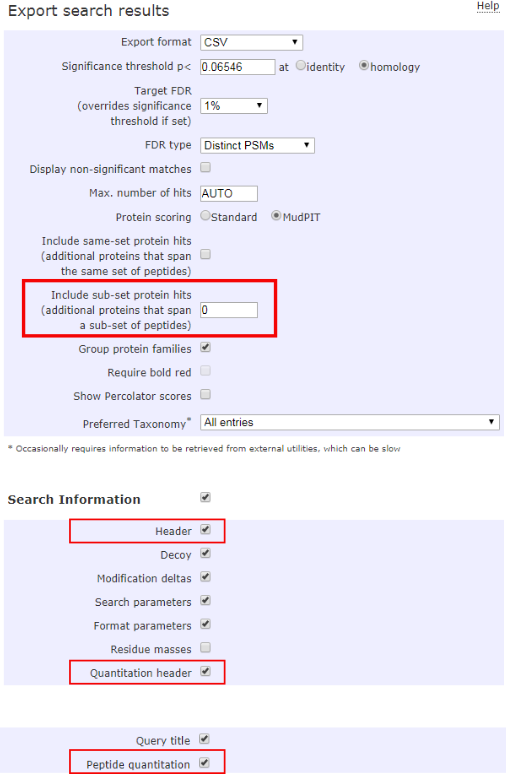
\includegraphics[width=0.45\linewidth]{images\mascot\mascot_export} \end{center}

The same peptide sequence under different PSM files can be assigned to
different protein IDs when
\href{https://www.ncbi.nlm.nih.gov/m/pubmed/21447708/}{inferring}
proteins from peptides using algorithms such as greedy set cover. To
avoid such ambiguity in protein inference, I typically enable the option
of \texttt{Merge\ MS/MS\ files\ into\ single\ search} in
\href{http://www.matrixscience.com/daemon.html}{Mascot Daemon}. If the
option is disabled, peptide sequences that have been assigned to
multiple protein IDs will be removed for now when constructing peptide
reports.

\begin{center}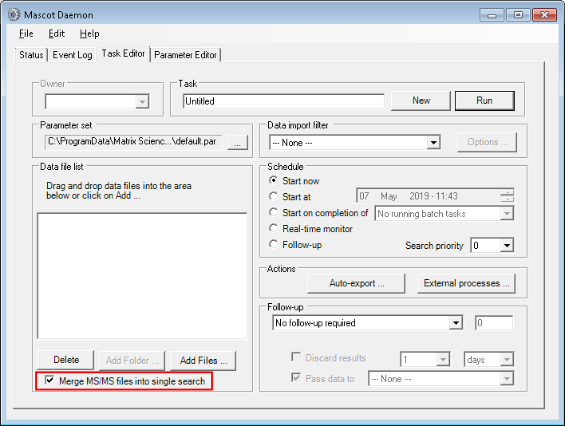
\includegraphics[width=0.45\linewidth]{images\mascot\mascot_daemon} \end{center}

The merged search may become increasingly demanding in computing powers
with growing data sets. In the example, I combined the MS peak lists
from the Hp-RP fractions within the same 10-plex TMT experiment, but not
the lists across experiments. This results in a total of six pieces of
PSM results in \texttt{Mascot} exports. To get us started, we go ahead
and copy the PSM files that we have prepared in \texttt{proteoQDA} over
to the working directory:

\begin{Shaded}
\begin{Highlighting}[]
\KeywordTok{library}\NormalTok{(proteoQDA)}
\KeywordTok{cptac_csv_1}\NormalTok{(dat_dir)}
\end{Highlighting}
\end{Shaded}

The workflow involves an \texttt{Excel} template containing the metadata
of multiplex experiment numbers, including TMT channels, LC/MS injection
indices, sample IDs, reference channels, \texttt{RAW} MS data file names
and addditional fields from the users. The default file name for the
experimental summary is \texttt{expt\_smry.xlsx}. If samples were
fractionated off-line prior to \texttt{LC/MS}, a second \texttt{Excel}
template will also be filled out to link multiple \texttt{RAW} MS file
names that are associated to the same sample IDs. The default file name
for the fractionation summary is \texttt{frac\_smry.xlsx}.\footnote{To
  extract the names of RAW files under a \texttt{raw\_dir} folder:
  \texttt{extract\_raws(raw\_dir)}} The description of the column keys
in the \texttt{Excel} files can be found from the help document by
entering \texttt{?proteoQ::load\_expts} from a \texttt{R} console. We
next copy over a pre-compiled \texttt{expt\_smry.xlsx} and a
\texttt{frac\_smry.xlsx} to the working directory:

\begin{Shaded}
\begin{Highlighting}[]
\KeywordTok{cptac_expt_1}\NormalTok{(dat_dir)}
\KeywordTok{cptac_frac_1}\NormalTok{(dat_dir)}
\end{Highlighting}
\end{Shaded}

We now have all the pieces that are required by \texttt{proteoQ} in
place. Let's have a quick glance at the \texttt{expt\_smry.xlsx} file.
We note that no reference channels were indicated under the column
\texttt{Reference}. With \texttt{proteoQ}, the \texttt{log2FC} of each
species in a given sample is calculated either (a) in relative to the
reference(s) within each multiplex TMT experiment or (b) to the mean of
all samples in the same experiment if reference(s) are absent. Hence,
the later approach will be employed to the examplary data set that we
are working with. In this special case, the mean of a given species in
each TMT experiment is the average of five \texttt{WHIM2} and five
\texttt{WHIM16} samples, which is biologically equivalent across TMT
experiments.

As a final step of the setup, we will load the experimental summary and
some precomputed results:

\begin{Shaded}
\begin{Highlighting}[]
\KeywordTok{library}\NormalTok{(proteoQ)}
\KeywordTok{load_expts}\NormalTok{()}
\end{Highlighting}
\end{Shaded}

\hypertarget{summarize-psms-to-peptides-and-proteins}{%
\subsubsection{Summarize PSMs to peptides and
proteins}\label{summarize-psms-to-peptides-and-proteins}}

\vspace{1.5cm}

\emph{Process PSMs} --- In this section, I demonstrate the summarisation
of PSM data to peptides and proteins. We start by processing PSM data
from \texttt{Mascot} outputs:

\begin{Shaded}
\begin{Highlighting}[]
\CommentTok{# Generate PSM reports}
\KeywordTok{normPSM}\NormalTok{(}
 \DataTypeTok{rptr_intco =} \DecValTok{1000}\NormalTok{,}
 \DataTypeTok{rm_craps =} \OtherTok{FALSE}\NormalTok{,}
 \DataTypeTok{rm_krts =} \OtherTok{FALSE}\NormalTok{,}
 \DataTypeTok{rm_outliers =} \OtherTok{FALSE}\NormalTok{,}
 \DataTypeTok{plot_violins =} \OtherTok{TRUE}
\NormalTok{)}

\CommentTok{# or accept the default parameters }
\KeywordTok{normPSM}\NormalTok{()}
\end{Highlighting}
\end{Shaded}

PSM outliers will be assessed at a basis of per peptide and per sample
at \texttt{rm\_outliers\ =\ TRUE}, which can be a slow process for large
data sets. To circumvent repeated efforts in the assessment of PSM
outliers, we may set \texttt{rm\_outliers\ =\ FALSE} and
\texttt{plot\_violins\ =\ TRUE} when first executing \texttt{normPSM()}.
We then visually inspect the violin plots of reporter-ion intensity.
Empirically, PSMs with reporter-ion intensity less than 1,000 are
trimmed and samples with median intensity that is 2/3 or less to the
average of majority samples are removed from further analysis.\footnote{The
  sample removal and PSM re-processing can be achieved by deleting the
  corresponding entries under the column \texttt{Sample\_ID} in
  \texttt{expt\_smry.xlsx}, followed by the re-load of the experiment,
  \texttt{load\_expts()}, and the re-execution of \texttt{normPSM()}
  with desired parameters.}

\vspace{1.5cm}

\emph{Summarize PSMs to peptides} --- We next summarise PSM to peptides.

\begin{Shaded}
\begin{Highlighting}[]
\CommentTok{# Generate peptide reports}
\KeywordTok{normPep}\NormalTok{(}
    \DataTypeTok{id =}\NormalTok{ pep_seq, }
    \DataTypeTok{method_psm_pep =}\NormalTok{ median, }
    \DataTypeTok{method_align =}\NormalTok{ MGKernel, }
    \DataTypeTok{range_log2r =} \KeywordTok{c}\NormalTok{(}\DecValTok{5}\NormalTok{, }\DecValTok{95}\NormalTok{), }
    \DataTypeTok{range_int =} \KeywordTok{c}\NormalTok{(}\DecValTok{5}\NormalTok{, }\DecValTok{95}\NormalTok{), }
    \DataTypeTok{n_comp =} \DecValTok{3}\NormalTok{, }
    \DataTypeTok{seed =} \DecValTok{749662}\NormalTok{, }
    \DataTypeTok{maxit =} \DecValTok{200}\NormalTok{, }
    \DataTypeTok{epsilon =} \FloatTok{1e-05}
\NormalTok{)}
\end{Highlighting}
\end{Shaded}

At \texttt{id\ =\ pep\_seq\_mod}, peptide sequences that are different
in variable modificaitons will be treated as different species. The
log2FC of peptide data will be aligned by median centering across
samples by default. If \texttt{method\_align\ =\ MGKernel} is chosen,
log2FC will be aligned under the assumption of multiple Gaussian
kernels.\footnote{Density kernel estimates can occasionally capture
  spikes in the profiles of log2FC for data alignment. Users will need
  to inspect the alignment of ratio histograms and may optimize the data
  normalization with different combinations of tuning parameters before
  proceeding to the next steps.} The parameter \texttt{n\_comp} defines
the number of Gaussian kernels and \texttt{seed} set a seed for
reproducible fittings. The parameters \texttt{range\_log2r} and
\texttt{range\_int} define the range of log2FC and the range of
reporter-ion intensity, respectively, for use in the scaling of standard
deviation across samples.

Let's compare the log2FC profiles with and without scaling
normalization:\footnote{\texttt{normPep()} will report log2FC results
  both before and after the scaling of standard deviations.}

\begin{Shaded}
\begin{Highlighting}[]
\CommentTok{# without the scaling of log2FC }
\KeywordTok{pepHist}\NormalTok{(}
 \DataTypeTok{scale_log2r =} \OtherTok{FALSE}\NormalTok{, }
 \DataTypeTok{ncol =} \DecValTok{10}
\NormalTok{)}

\CommentTok{# with the scaling of log2FC }
\KeywordTok{pepHist}\NormalTok{(}
 \DataTypeTok{scale_log2r =} \OtherTok{TRUE}\NormalTok{, }
 \DataTypeTok{ncol =} \DecValTok{10}
\NormalTok{)}
\end{Highlighting}
\end{Shaded}

There are 60 panels of of histograms in each plot, which may not be easy
to explore as a whole. In stead, we will break the plots down by their
data origins. We begin with modifying the \texttt{expt\_smry.xlsx} file
by adding the columns \texttt{BI}, \texttt{JHU} and \texttt{PNNL}. Each
of the new columns includes sample entries that are tied to their
laboratory origins.

\href{https://www.youtube.com/embed/3B5et8VY3hE}{\includegraphics{https://img.youtube.com/vi/3B5et8VY3hE/0.jpg}}

We now are ready to plot histograms for each subset of data.\footnote{system
  files will be automatically updated from the modified
  \texttt{expt\_smry.xlsx}} In this document, we only display the plots
using the \texttt{BI} subset:

\begin{Shaded}
\begin{Highlighting}[]
\CommentTok{# without the scaling of log2FC }
\KeywordTok{pepHist}\NormalTok{(}
 \DataTypeTok{scale_log2r =} \OtherTok{FALSE}\NormalTok{, }
 \DataTypeTok{col_select =}\NormalTok{ BI,}
 \DataTypeTok{filename =}\NormalTok{ Hist_BI_N.png, }
 \DataTypeTok{ncol =} \DecValTok{5}
\NormalTok{)}

\CommentTok{# with the scaling of log2FC }
\KeywordTok{pepHist}\NormalTok{(}
 \DataTypeTok{scale_log2r =} \OtherTok{TRUE}\NormalTok{, }
 \DataTypeTok{col_select =}\NormalTok{ BI,}
 \DataTypeTok{filename =}\NormalTok{ Hist_BI_Z.png, }
 \DataTypeTok{ncol =} \DecValTok{5}
\NormalTok{)}
\end{Highlighting}
\end{Shaded}

\begin{verbatim}
*NB*: We interactively told `pepHist()` that we are interested in sample entries under the newly created `BI` column. We also supply a file name, assuming that we want to keep the earlierly generated plots with default file names of `Peptide_Histogram_N.png` and `Peptide_Histogram_Z.png`. 
\end{verbatim}

\textbackslash{}begin\{figure\}

\{\centering 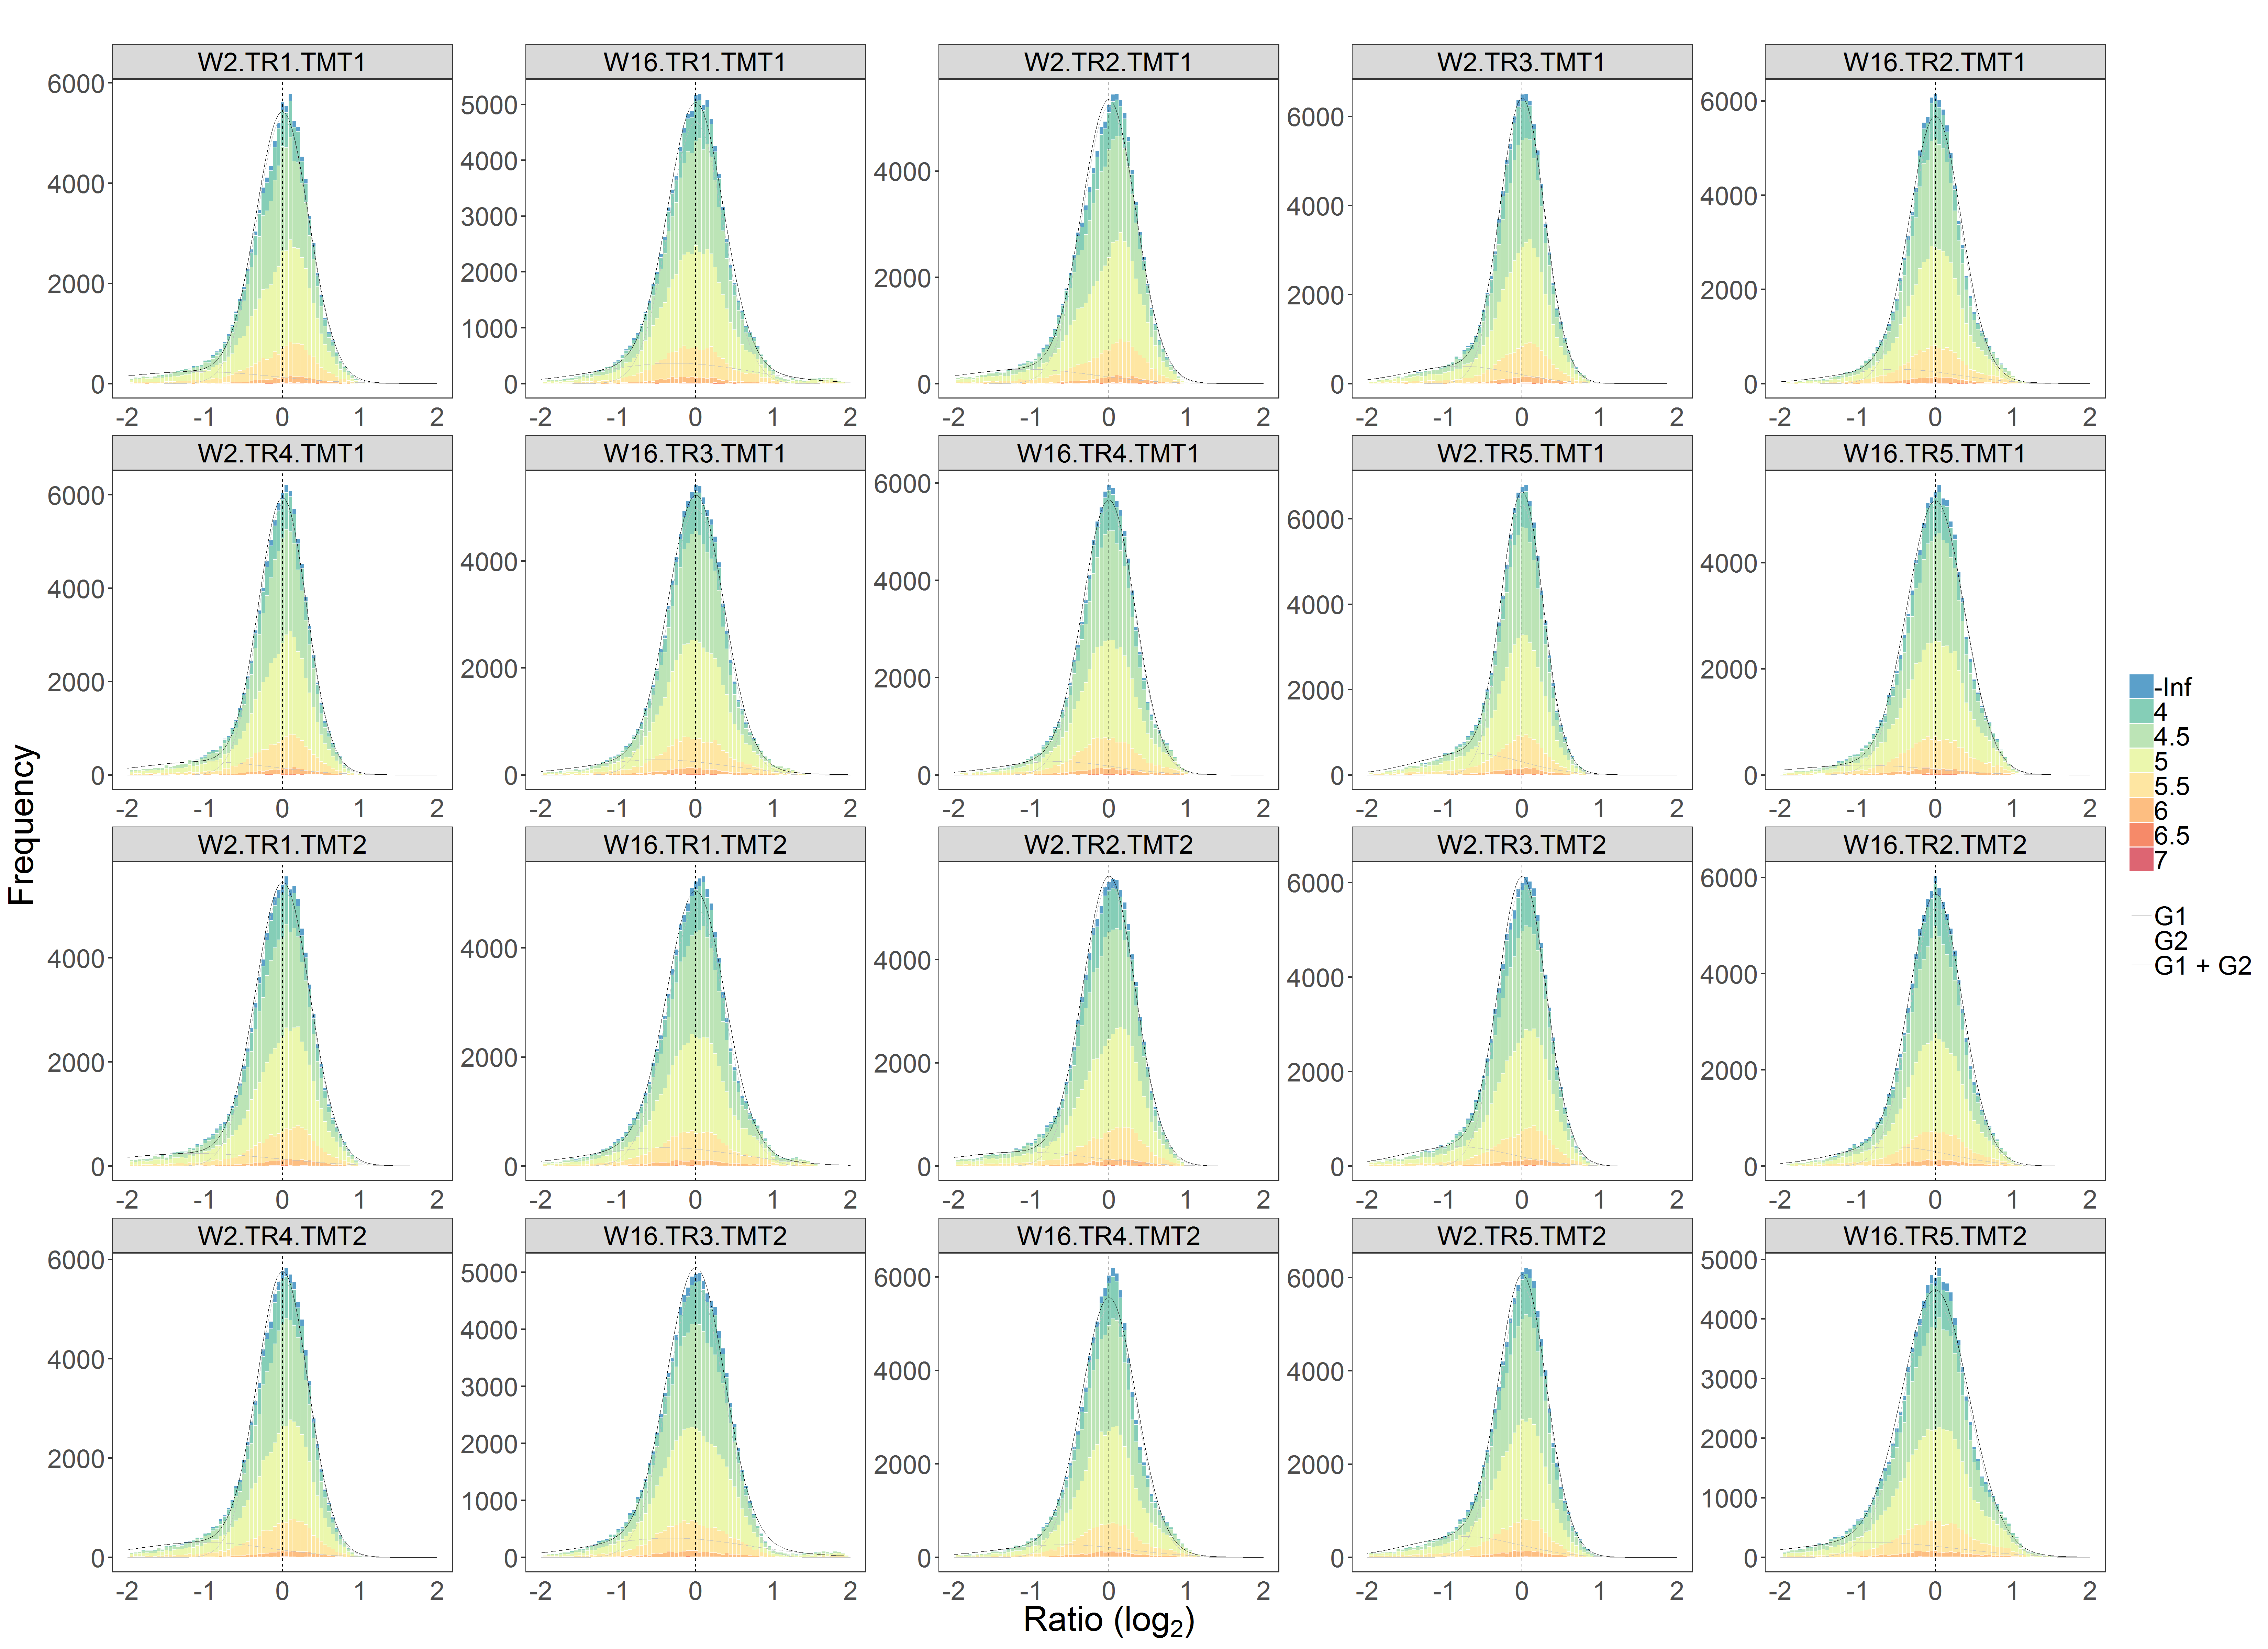
\includegraphics[width=0.45\linewidth]{images\peptide\histogram\peptide_bi_gl1_n}
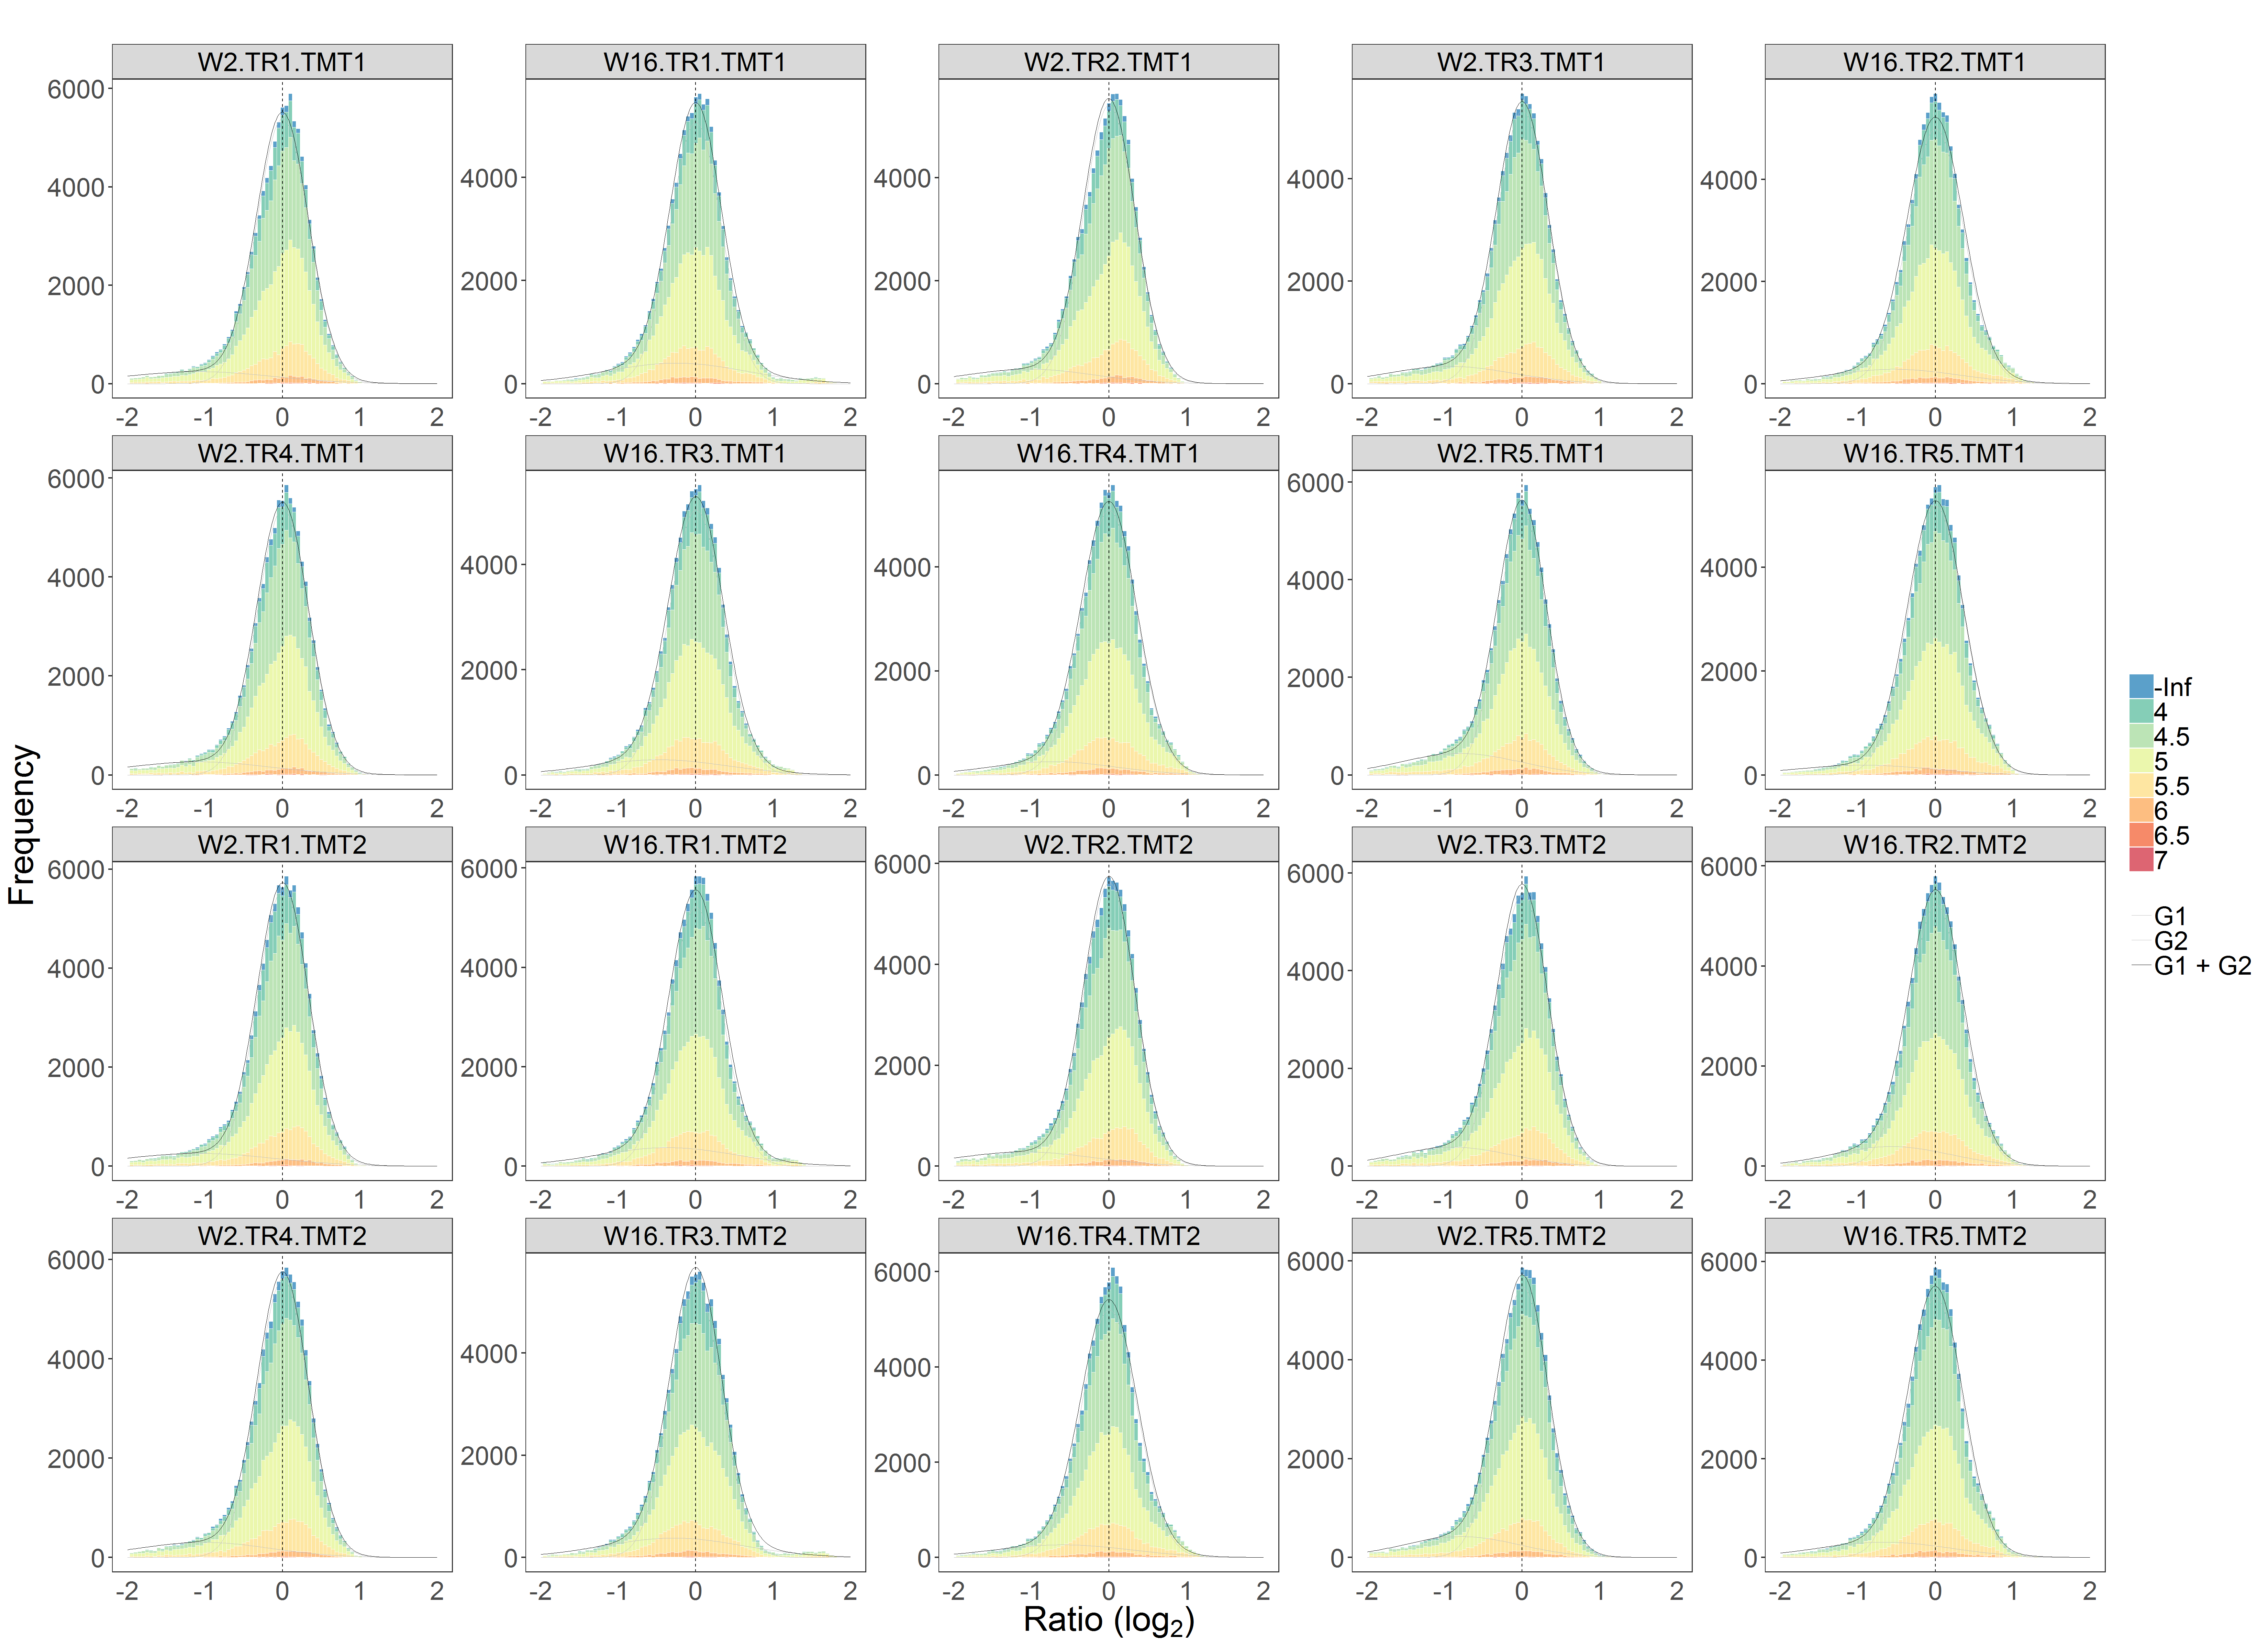
\includegraphics[width=0.45\linewidth]{images\peptide\histogram\peptide_bi_gl1_z}

\}

\textbackslash{}caption\{\textbf{Figure 1.} Histograms of peptide
log2FC. Left: \texttt{scale\_log2r\ =\ FALSE}; right,
\texttt{scale\_log2r\ =\ TRUE}\}\label{fig:Peptide histogram F}
\textbackslash{}end\{figure\}

As expected, the widths of log2FC profiles become more consistent after
the scaling normalization. However, such adjustment may cause artifacts
when the standard deviaiton across samples are genuinely different. I
typically test \texttt{scale\_log2r} at both \texttt{TRUE} and
\texttt{FALSE}, then make a choice in data scaling together with my a
priori knowledge of the characteristics of both samples and
references.\footnote{The default is \texttt{scale\_log2r\ =\ TRUE}
  throughout the package. When calling functions involved parameter
  \texttt{scale\_log2r}, users can specify explicitly
  \texttt{scale\_log2r\ =\ FALSE} or define its value under the global
  environment.} I will use the same data set to illustrate the impacts
of references in scaling normalization in
\protect\hyperlink{ux5cux23ux5cux23ux5cux2520Labux5cux25201}{Lab 1}.
Alignment of log2FC against housekeeping or normalizer protein(s) is
also available. This seems suitable when the quantities of proteins of
interest are different across samples where the assumption of
constitutive expression for the vast majority of proteins may not hold.

\vspace{1.5cm}

\emph{Summarize peptides to proteins} --- We then summarise peptides to
proteins using a two-component Gaussian kernel.

\begin{Shaded}
\begin{Highlighting}[]
\CommentTok{# Generate protein reports}
\KeywordTok{normPrn}\NormalTok{(}
    \DataTypeTok{id =}\NormalTok{ gene, }
    \DataTypeTok{method_pep_prn =}\NormalTok{ median, }
    \DataTypeTok{method_align =}\NormalTok{ MGKernel, }
    \DataTypeTok{range_log2r =} \KeywordTok{c}\NormalTok{(}\DecValTok{5}\NormalTok{, }\DecValTok{95}\NormalTok{), }
    \DataTypeTok{range_int =} \KeywordTok{c}\NormalTok{(}\DecValTok{5}\NormalTok{, }\DecValTok{95}\NormalTok{), }
    \DataTypeTok{n_comp =} \DecValTok{2}\NormalTok{, }
    \DataTypeTok{seed =} \DecValTok{749662}\NormalTok{, }
    \DataTypeTok{fasta =} \StringTok{"C:}\CharTok{\textbackslash{}\textbackslash{}}\StringTok{Results}\CharTok{\textbackslash{}\textbackslash{}}\StringTok{DB}\CharTok{\textbackslash{}\textbackslash{}}\StringTok{Refseq}\CharTok{\textbackslash{}\textbackslash{}}\StringTok{RefSeq_HM_Frozen_20130727.fasta"}\NormalTok{, }
    \DataTypeTok{maxit =} \DecValTok{200}\NormalTok{, }
    \DataTypeTok{epsilon =} \FloatTok{1e-05}
\NormalTok{)}
\end{Highlighting}
\end{Shaded}

Similar to the peptide summary, we inspect the alignment and the scaling
of ratio profiles, and re-normalize the data if needed.\footnote{Prameter
  \texttt{fasta} is solely used for the calculation of protein percent
  coverage. Precomputed data will be used if no \texttt{fasta} database
  is provided.}

\begin{Shaded}
\begin{Highlighting}[]
\CommentTok{# without the scaling of log2FC}
\KeywordTok{prnHist}\NormalTok{(}
 \DataTypeTok{scale_log2r =} \OtherTok{FALSE}\NormalTok{, }
 \DataTypeTok{ncol =} \DecValTok{10}
\NormalTok{)}

\CommentTok{# with the scaling of log2FC}
\KeywordTok{prnHist}\NormalTok{(}
 \DataTypeTok{scale_log2r =} \OtherTok{TRUE}\NormalTok{, }
 \DataTypeTok{ncol =} \DecValTok{10}
\NormalTok{)}
\end{Highlighting}
\end{Shaded}

\hypertarget{application-part-ii}{%
\subsection{Application -- Part II}\label{application-part-ii}}

In this section I illustrate the following applications of
\texttt{proteoQ}:

\begin{itemize}
\tightlist
\item
  Basic informatic analysis and linear modeling against the peptide and
  protein data.
\end{itemize}

\hypertarget{mds-and-pca-plots}{%
\subsubsection{MDS and PCA plots}\label{mds-and-pca-plots}}

In this section, we visualize MDS, PCA and Euclidean distance against
the peptide data at \texttt{scale\_log2r\ =\ TRUE}. We start with metric
MDS for peptide data:

\begin{Shaded}
\begin{Highlighting}[]
\CommentTok{# data from all three laboratories}
\KeywordTok{pepMDS}\NormalTok{(}
    \DataTypeTok{show_ids =} \OtherTok{FALSE}
\NormalTok{)}
\end{Highlighting}
\end{Shaded}

\textbackslash{}begin\{figure\}

\{\centering 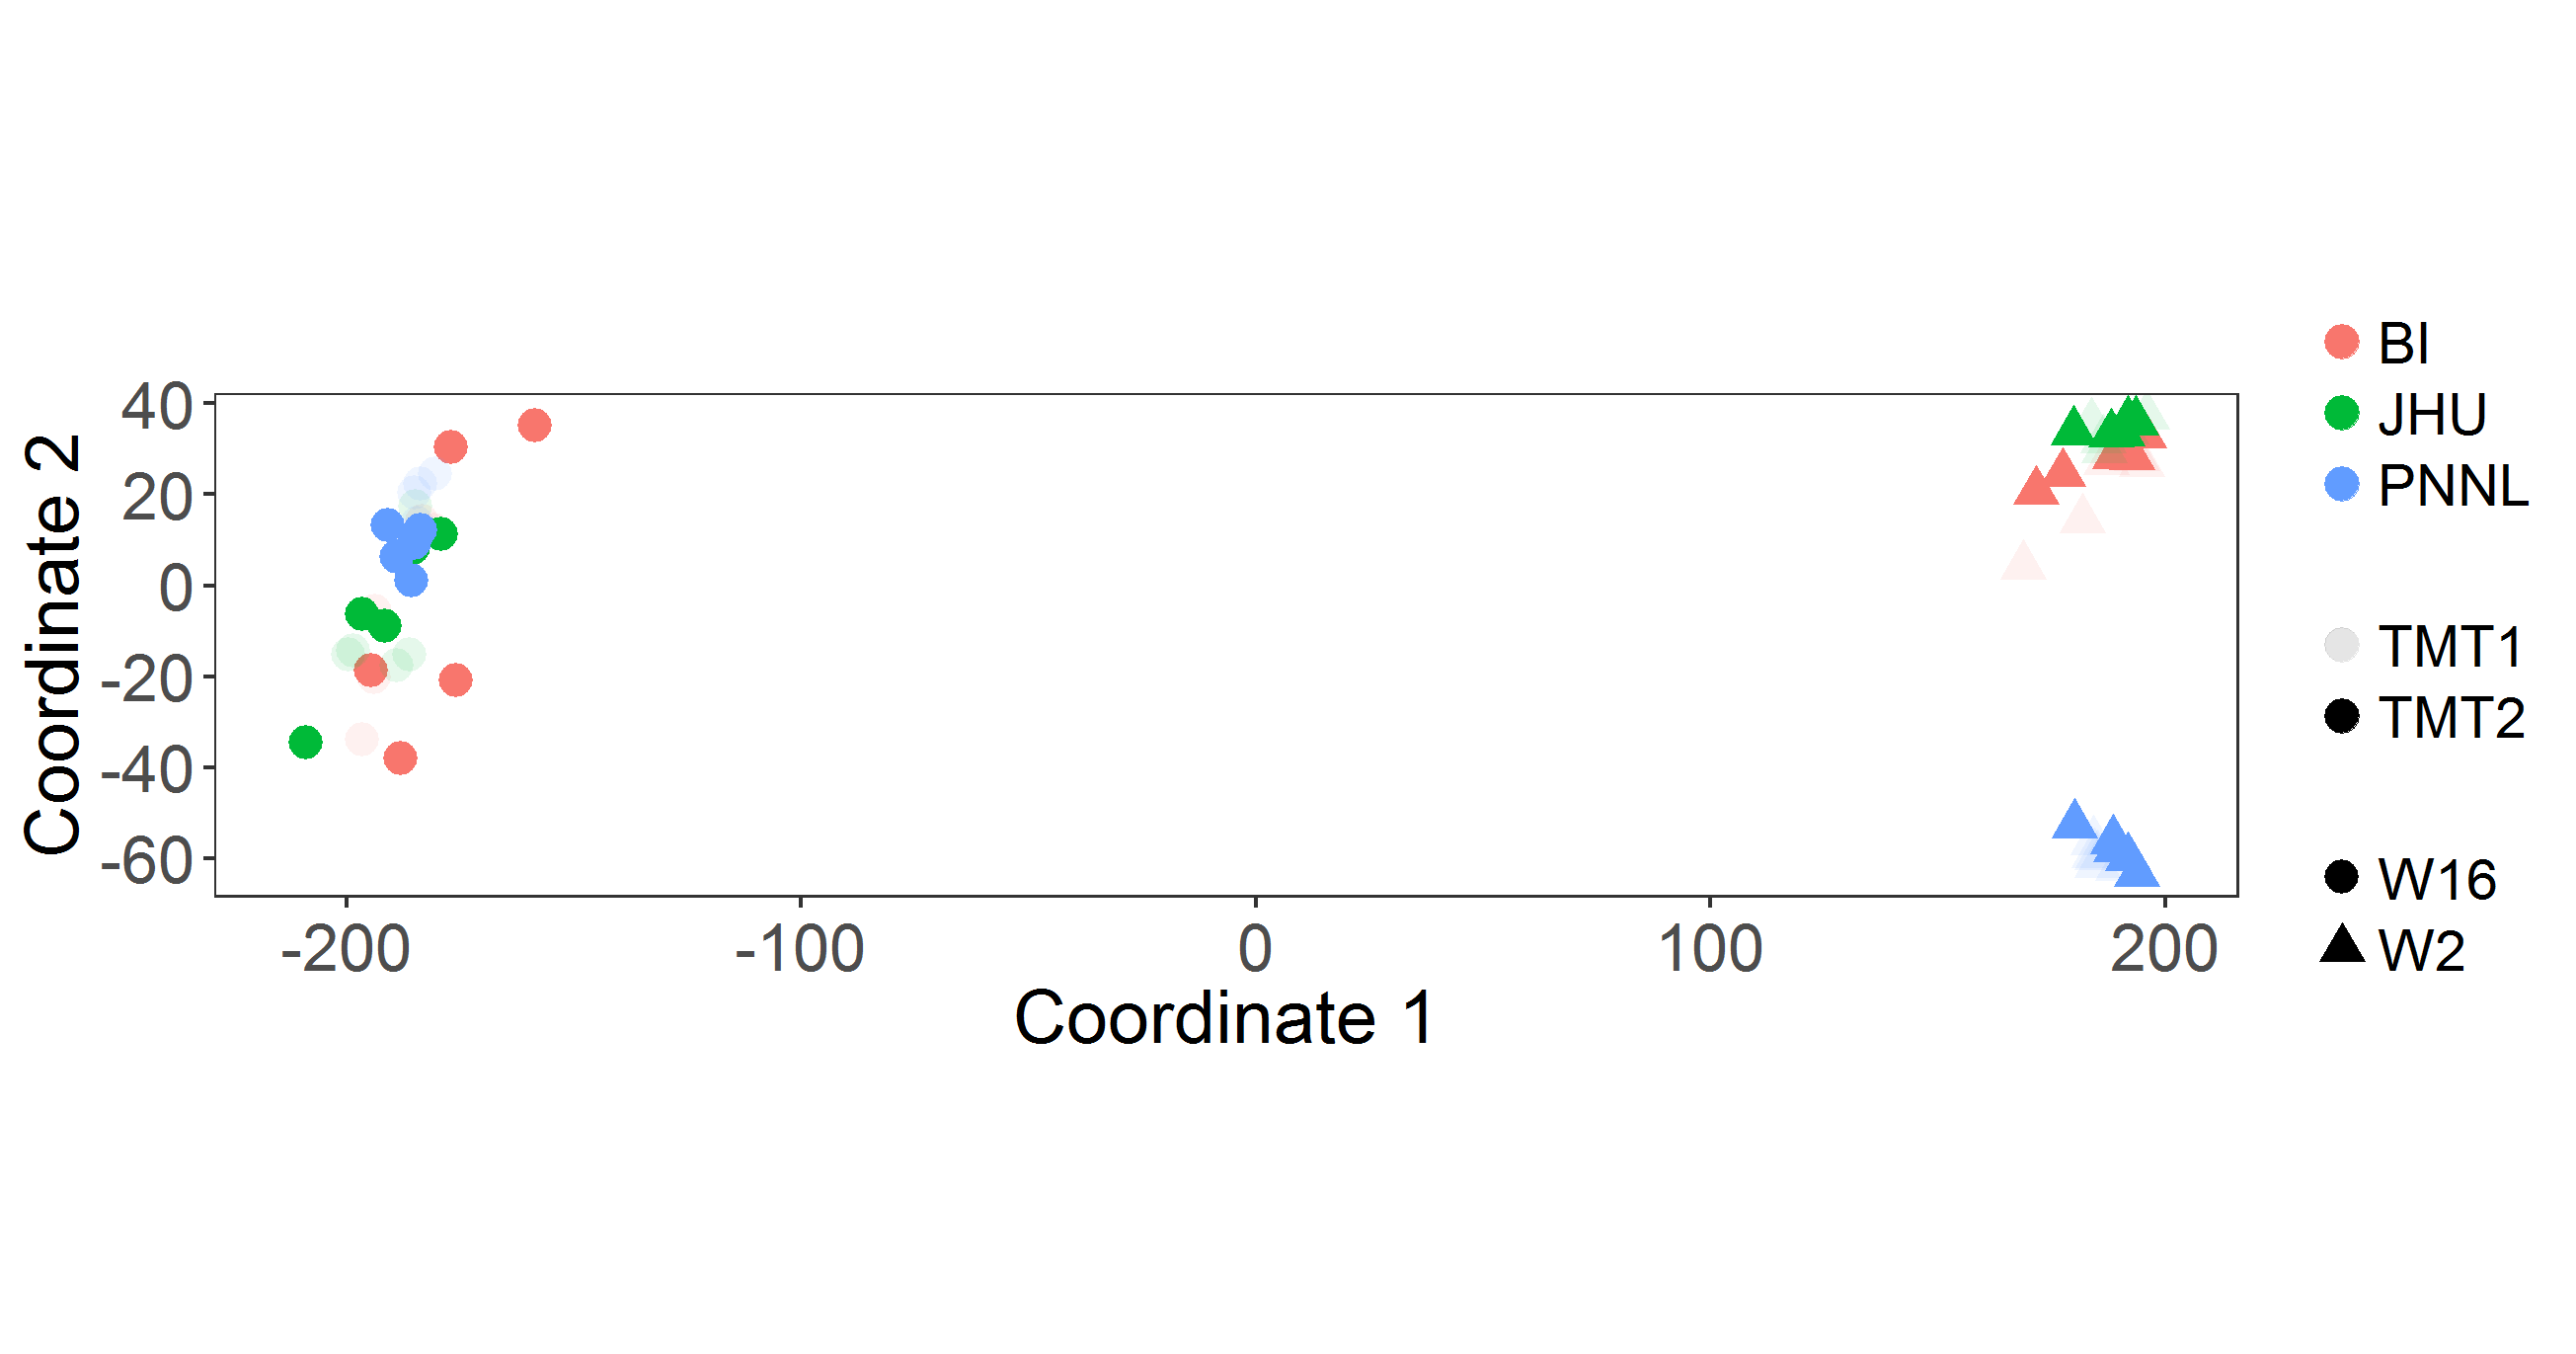
\includegraphics[width=0.45\linewidth]{images\peptide\mds\peptide_mds}

\}

\textbackslash{}caption\{\textbf{Figure 2A.} MDS of peptide log2FC at
\texttt{scale\_log2r\ =\ TRUE}\}\label{fig:Peptide_MDS}
\textbackslash{}end\{figure\}

It is clear that the WHIM2 and WHIM16 samples are well separated by the
Euclidean distance of log2FC (\textbf{Figure 2A}). We next take the
\texttt{JHU} data subset as an example to explore batch effects in the
proteomic sample handling:

\begin{Shaded}
\begin{Highlighting}[]
\CommentTok{# `JHU` subset}
\KeywordTok{pepMDS}\NormalTok{(}
  \DataTypeTok{col_select =}\NormalTok{ JHU,}
  \DataTypeTok{filename =}\NormalTok{ MDS_JHU.png,}
  \DataTypeTok{show_ids =} \OtherTok{FALSE}
\NormalTok{)}
\end{Highlighting}
\end{Shaded}

\begin{figure}

{\centering 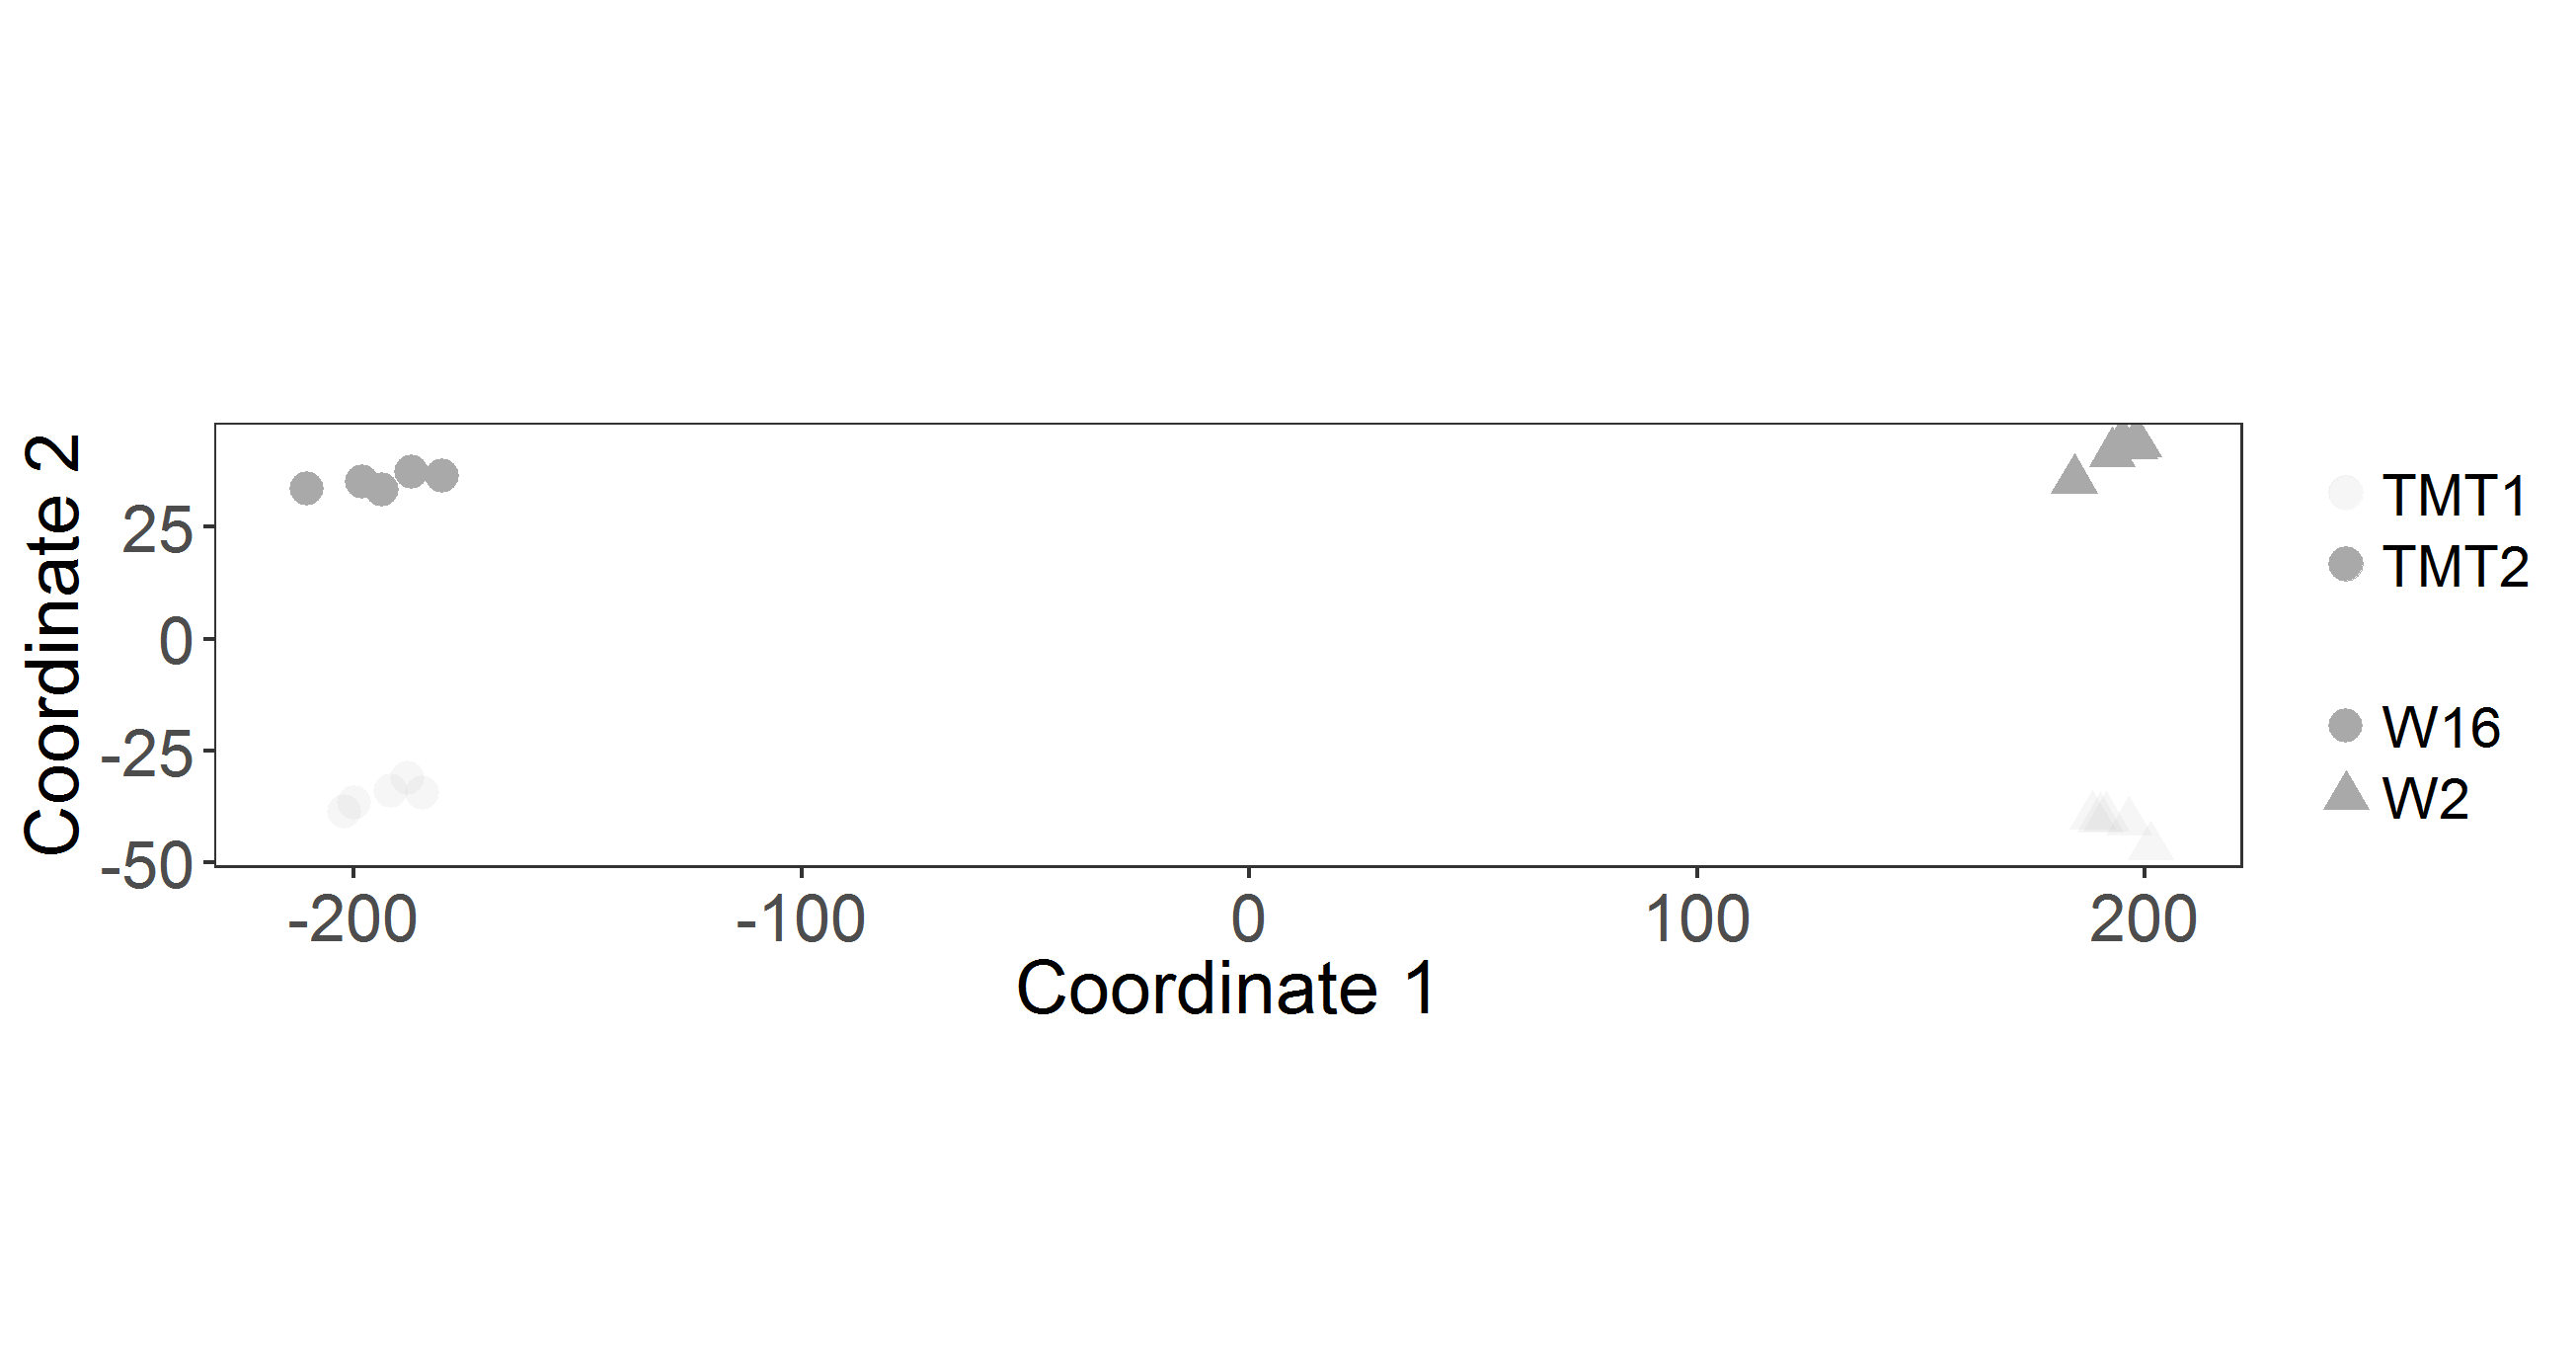
\includegraphics[width=0.45\linewidth]{images\peptide\mds\mds_jhu} 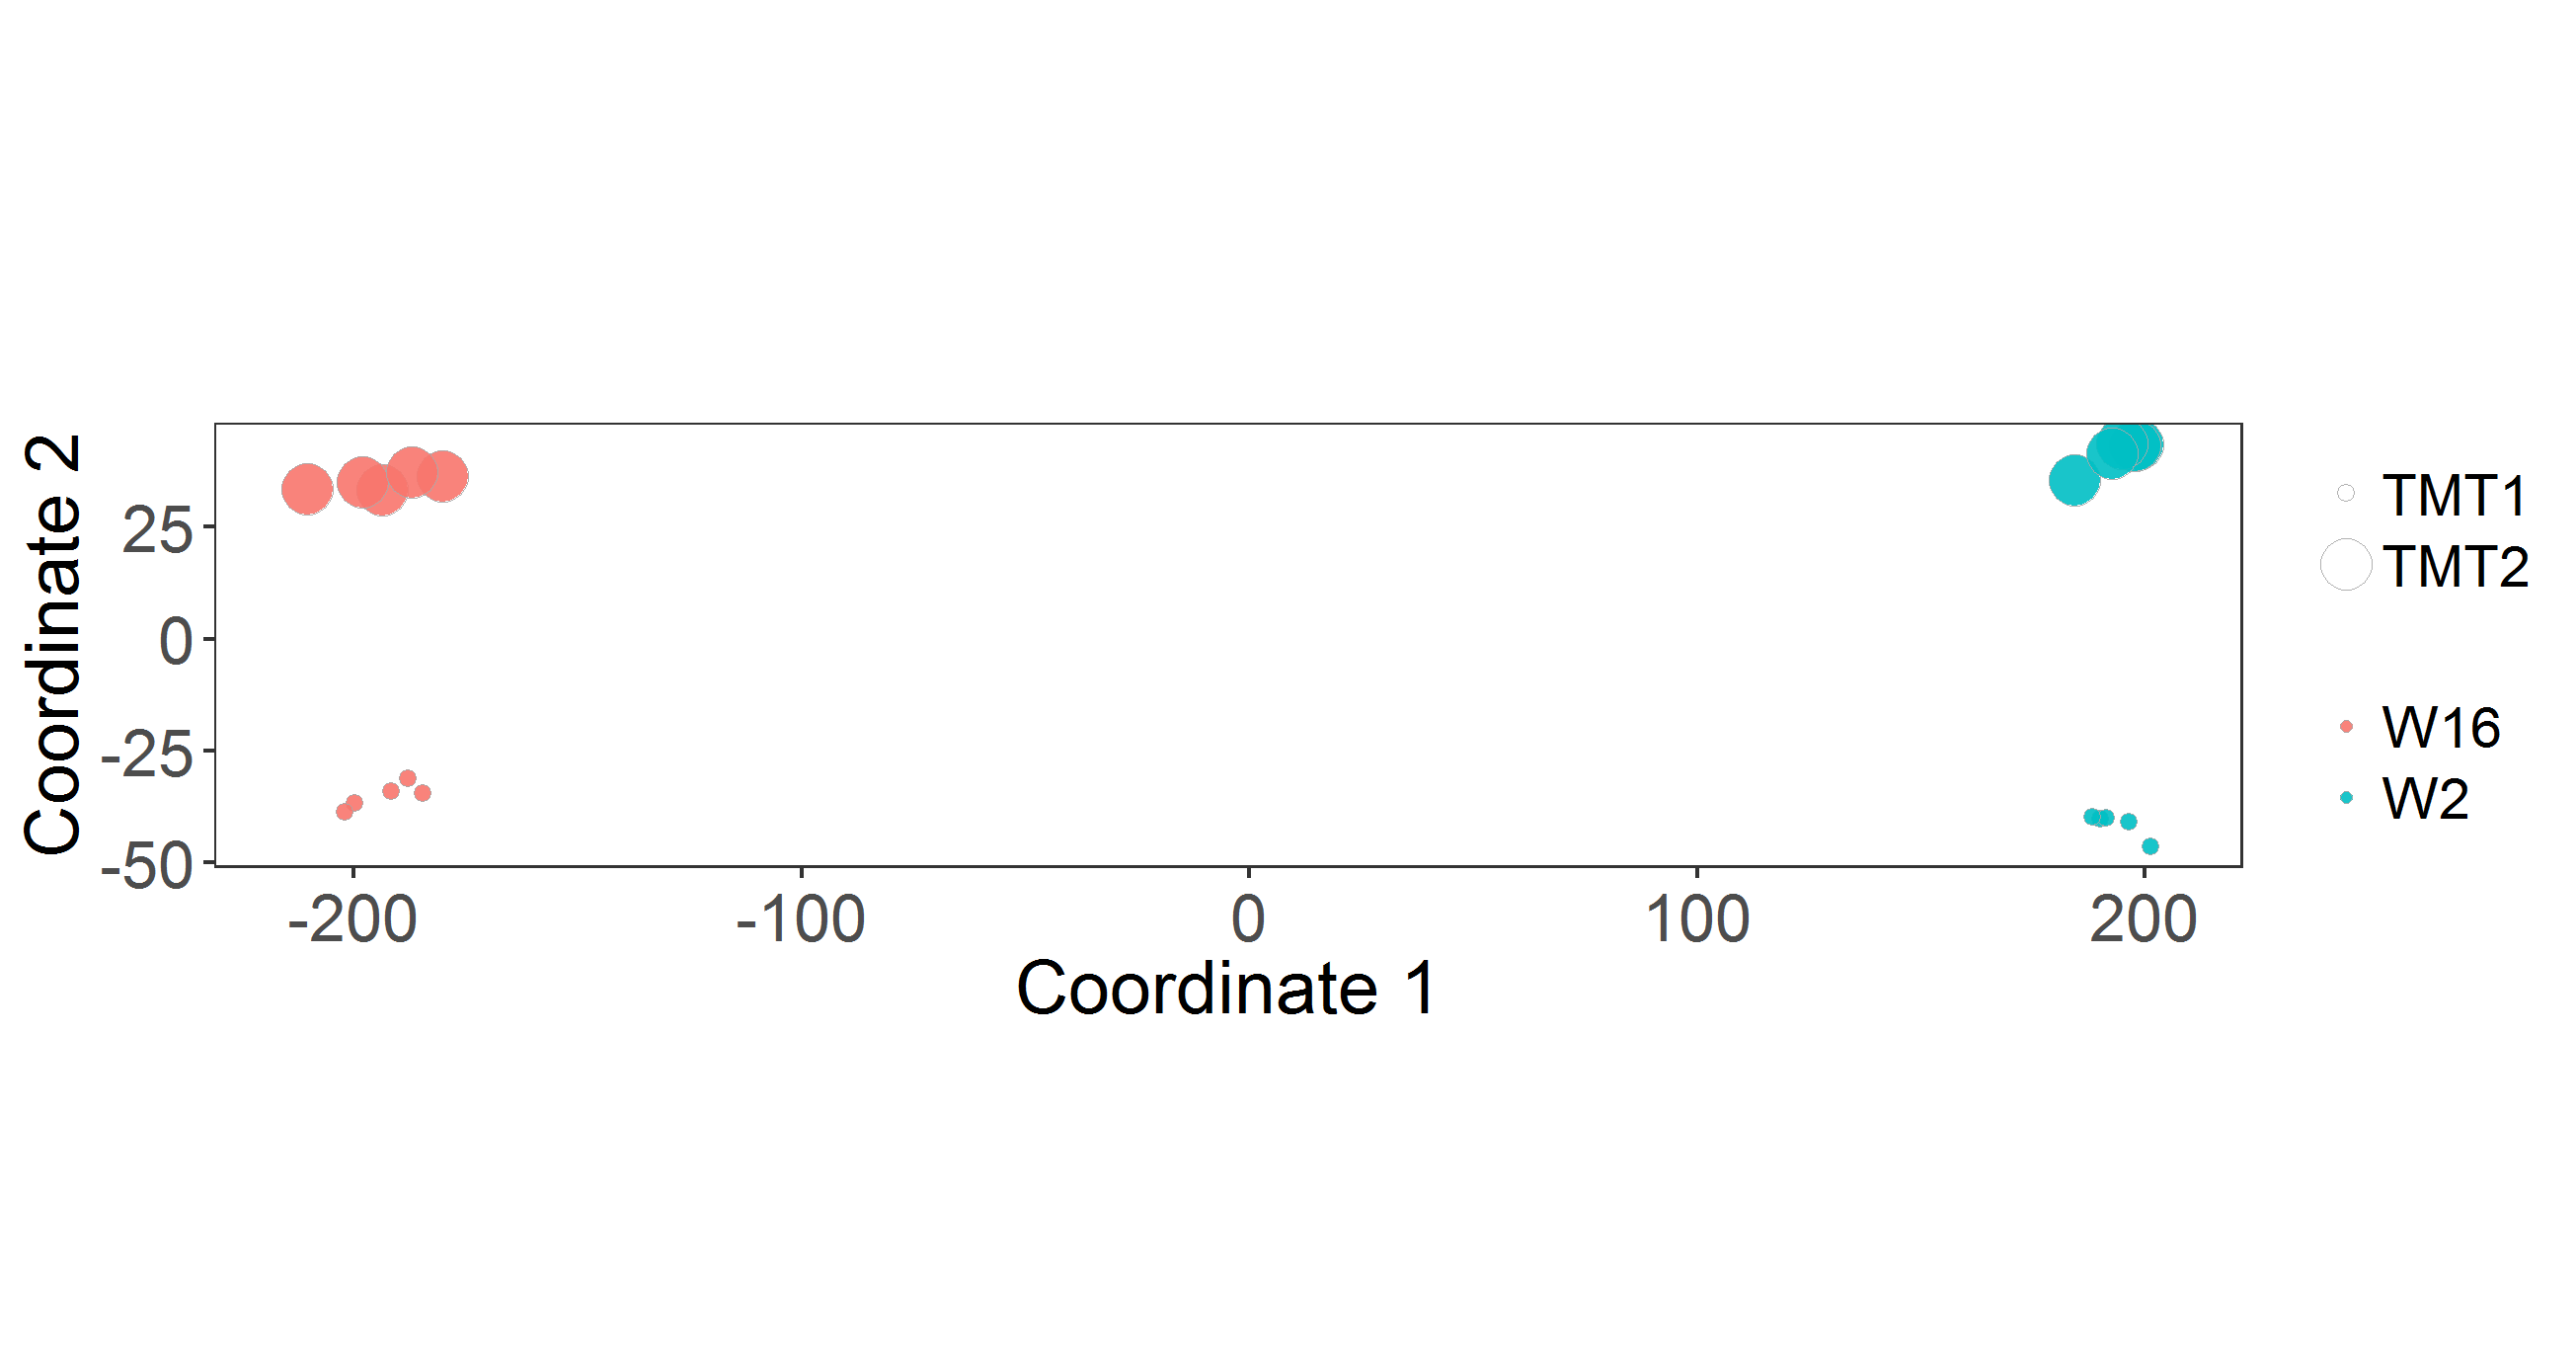
\includegraphics[width=0.45\linewidth]{images\peptide\mds\mds_jhu_new_aes} 

}

\caption{**Figure 2B-2C.** MDS of peptide log2FC for the `JHU` subset. Left: original aesthetics; right, modefied aesthetics}\label{fig:Peptide_JHU_MDS}
\end{figure}

We immediately spot that all samples are coded with the same color
(\textbf{Figure 2B}). This is not a surprise as the values under column
\texttt{expt\_smry.xlsx::Color} are exclusively \texttt{JHU} for the
\texttt{JHU} subset. For similar reasons, the two different batches of
\texttt{TMT1} and \texttt{TMT2} are distinguished by transparency, which
is governed by column \texttt{expt\_smry.xlsx::Alpha}. We may wish to
modify the aesthetics using different keys: e.g., color coding by WHIMs
and size coding by batches, without the recourse of writing new R
scripts. One solution is to link the attributes and sample IDs by
creating additional columns in \texttt{expt\_smry.xlsx}. In this
example, we have had coincidentally prepared the column \texttt{Shape}
and \texttt{Alpha} to code WHIMs and batches, respectively. Therefore,
we can recycle them directly to make a new plot (\textbf{Figure 2C}):

\begin{Shaded}
\begin{Highlighting}[]
\CommentTok{# `JHU` subset}
\KeywordTok{pepMDS}\NormalTok{(}
  \DataTypeTok{col_select =}\NormalTok{ JHU,}
  \DataTypeTok{col_fill =}\NormalTok{ Shape, }\CommentTok{# WHIMs  }
  \DataTypeTok{col_size =}\NormalTok{ Alpha, }\CommentTok{# batches}
  \DataTypeTok{filename =}\NormalTok{ MDS_JHU_new_aes.png,}
  \DataTypeTok{show_ids =} \OtherTok{FALSE}
\NormalTok{)}
\end{Highlighting}
\end{Shaded}

The \texttt{prnMDS} performs \texttt{MDS} for protein data. For
\texttt{PCA} analysis, the corresponding functions are \texttt{pepPCA}
and \texttt{prnPCA} for peptide and protein data, respectively.

While \texttt{MDS} approximates Euclidean distances at a low dimensional
space. Sometime it may be useful to have an accurate view of the
distance matrix. Functions \texttt{pepEucDist} and \texttt{prnEucDist}
plot the heat maps of Euclidean distance matrix for peptides and
proteins, respectively. They are wrappers of
(\href{https://cran.r-project.org/web/packages/pheatmap/pheatmap.pdf}{\texttt{pheatmap}})
and inherit many parameters therein. Supposed that we are interested in
visualizing the distance matrix for the \texttt{JHU} subset:

\begin{Shaded}
\begin{Highlighting}[]
\CommentTok{# `JHU` subset}
\KeywordTok{pepEucDist}\NormalTok{(}
    \DataTypeTok{col_select =}\NormalTok{ JHU,}
    \DataTypeTok{annot_cols =} \KeywordTok{c}\NormalTok{(}\StringTok{"Shape"}\NormalTok{, }\StringTok{"Alpha"}\NormalTok{),}
    \DataTypeTok{annot_colnames =} \KeywordTok{c}\NormalTok{(}\StringTok{"WHIM"}\NormalTok{, }\StringTok{"Batch"}\NormalTok{), }

    \CommentTok{# parameters from `pheatmap`}
    \DataTypeTok{display_numbers =} \OtherTok{TRUE}\NormalTok{, }
    \DataTypeTok{number_color =} \StringTok{"grey30"}\NormalTok{, }
    \DataTypeTok{number_format =} \StringTok{"%.1f"}\NormalTok{,}
    
    \DataTypeTok{clustering_distance_rows =} \StringTok{"euclidean"}\NormalTok{, }
    \DataTypeTok{clustering_distance_cols =} \StringTok{"euclidean"}\NormalTok{, }
    
    \DataTypeTok{fontsize =} \DecValTok{16}\NormalTok{, }
    \DataTypeTok{fontsize_row =} \DecValTok{20}\NormalTok{, }
    \DataTypeTok{fontsize_col =} \DecValTok{20}\NormalTok{, }
    \DataTypeTok{fontsize_number =} \DecValTok{8}\NormalTok{, }
    
    \DataTypeTok{cluster_rows =} \OtherTok{TRUE}\NormalTok{,}
    \DataTypeTok{show_rownames =} \OtherTok{TRUE}\NormalTok{,}
    \DataTypeTok{show_colnames =} \OtherTok{TRUE}\NormalTok{,}
    \DataTypeTok{border_color =} \StringTok{"grey60"}\NormalTok{, }
    \DataTypeTok{cellwidth =} \DecValTok{24}\NormalTok{, }
    \DataTypeTok{cellheight =} \DecValTok{24}\NormalTok{, }
    \DataTypeTok{width =} \DecValTok{14}\NormalTok{,}
    \DataTypeTok{height =} \DecValTok{12}\NormalTok{, }
    
    \DataTypeTok{filename =}\NormalTok{ EucDist_JHU.png}
\NormalTok{)}
\end{Highlighting}
\end{Shaded}

Parameter \texttt{annot\_cols} defines the tracks to be displayed on the
top of distrance-matrix plots. In this example, we have choosen
\texttt{expt\_smry.xlsx::Shape} and \texttt{expt\_smry.xlsx::Alpha},
which encodes the WHIM subtypes and the batch numbers, respectively.
Parameter \texttt{annot\_colnames} allows us to rename the tracks from
\texttt{Shape} and \texttt{Alpha} to \texttt{WHIM} and \texttt{Batch},
respectively, for better intuition. We can alternatively add columns
\texttt{WHIM} and \texttt{Batch} if we choose not to recycle columns
\texttt{Shape} and \texttt{Alpha}.

\textbackslash{}begin\{figure\}

\{\centering 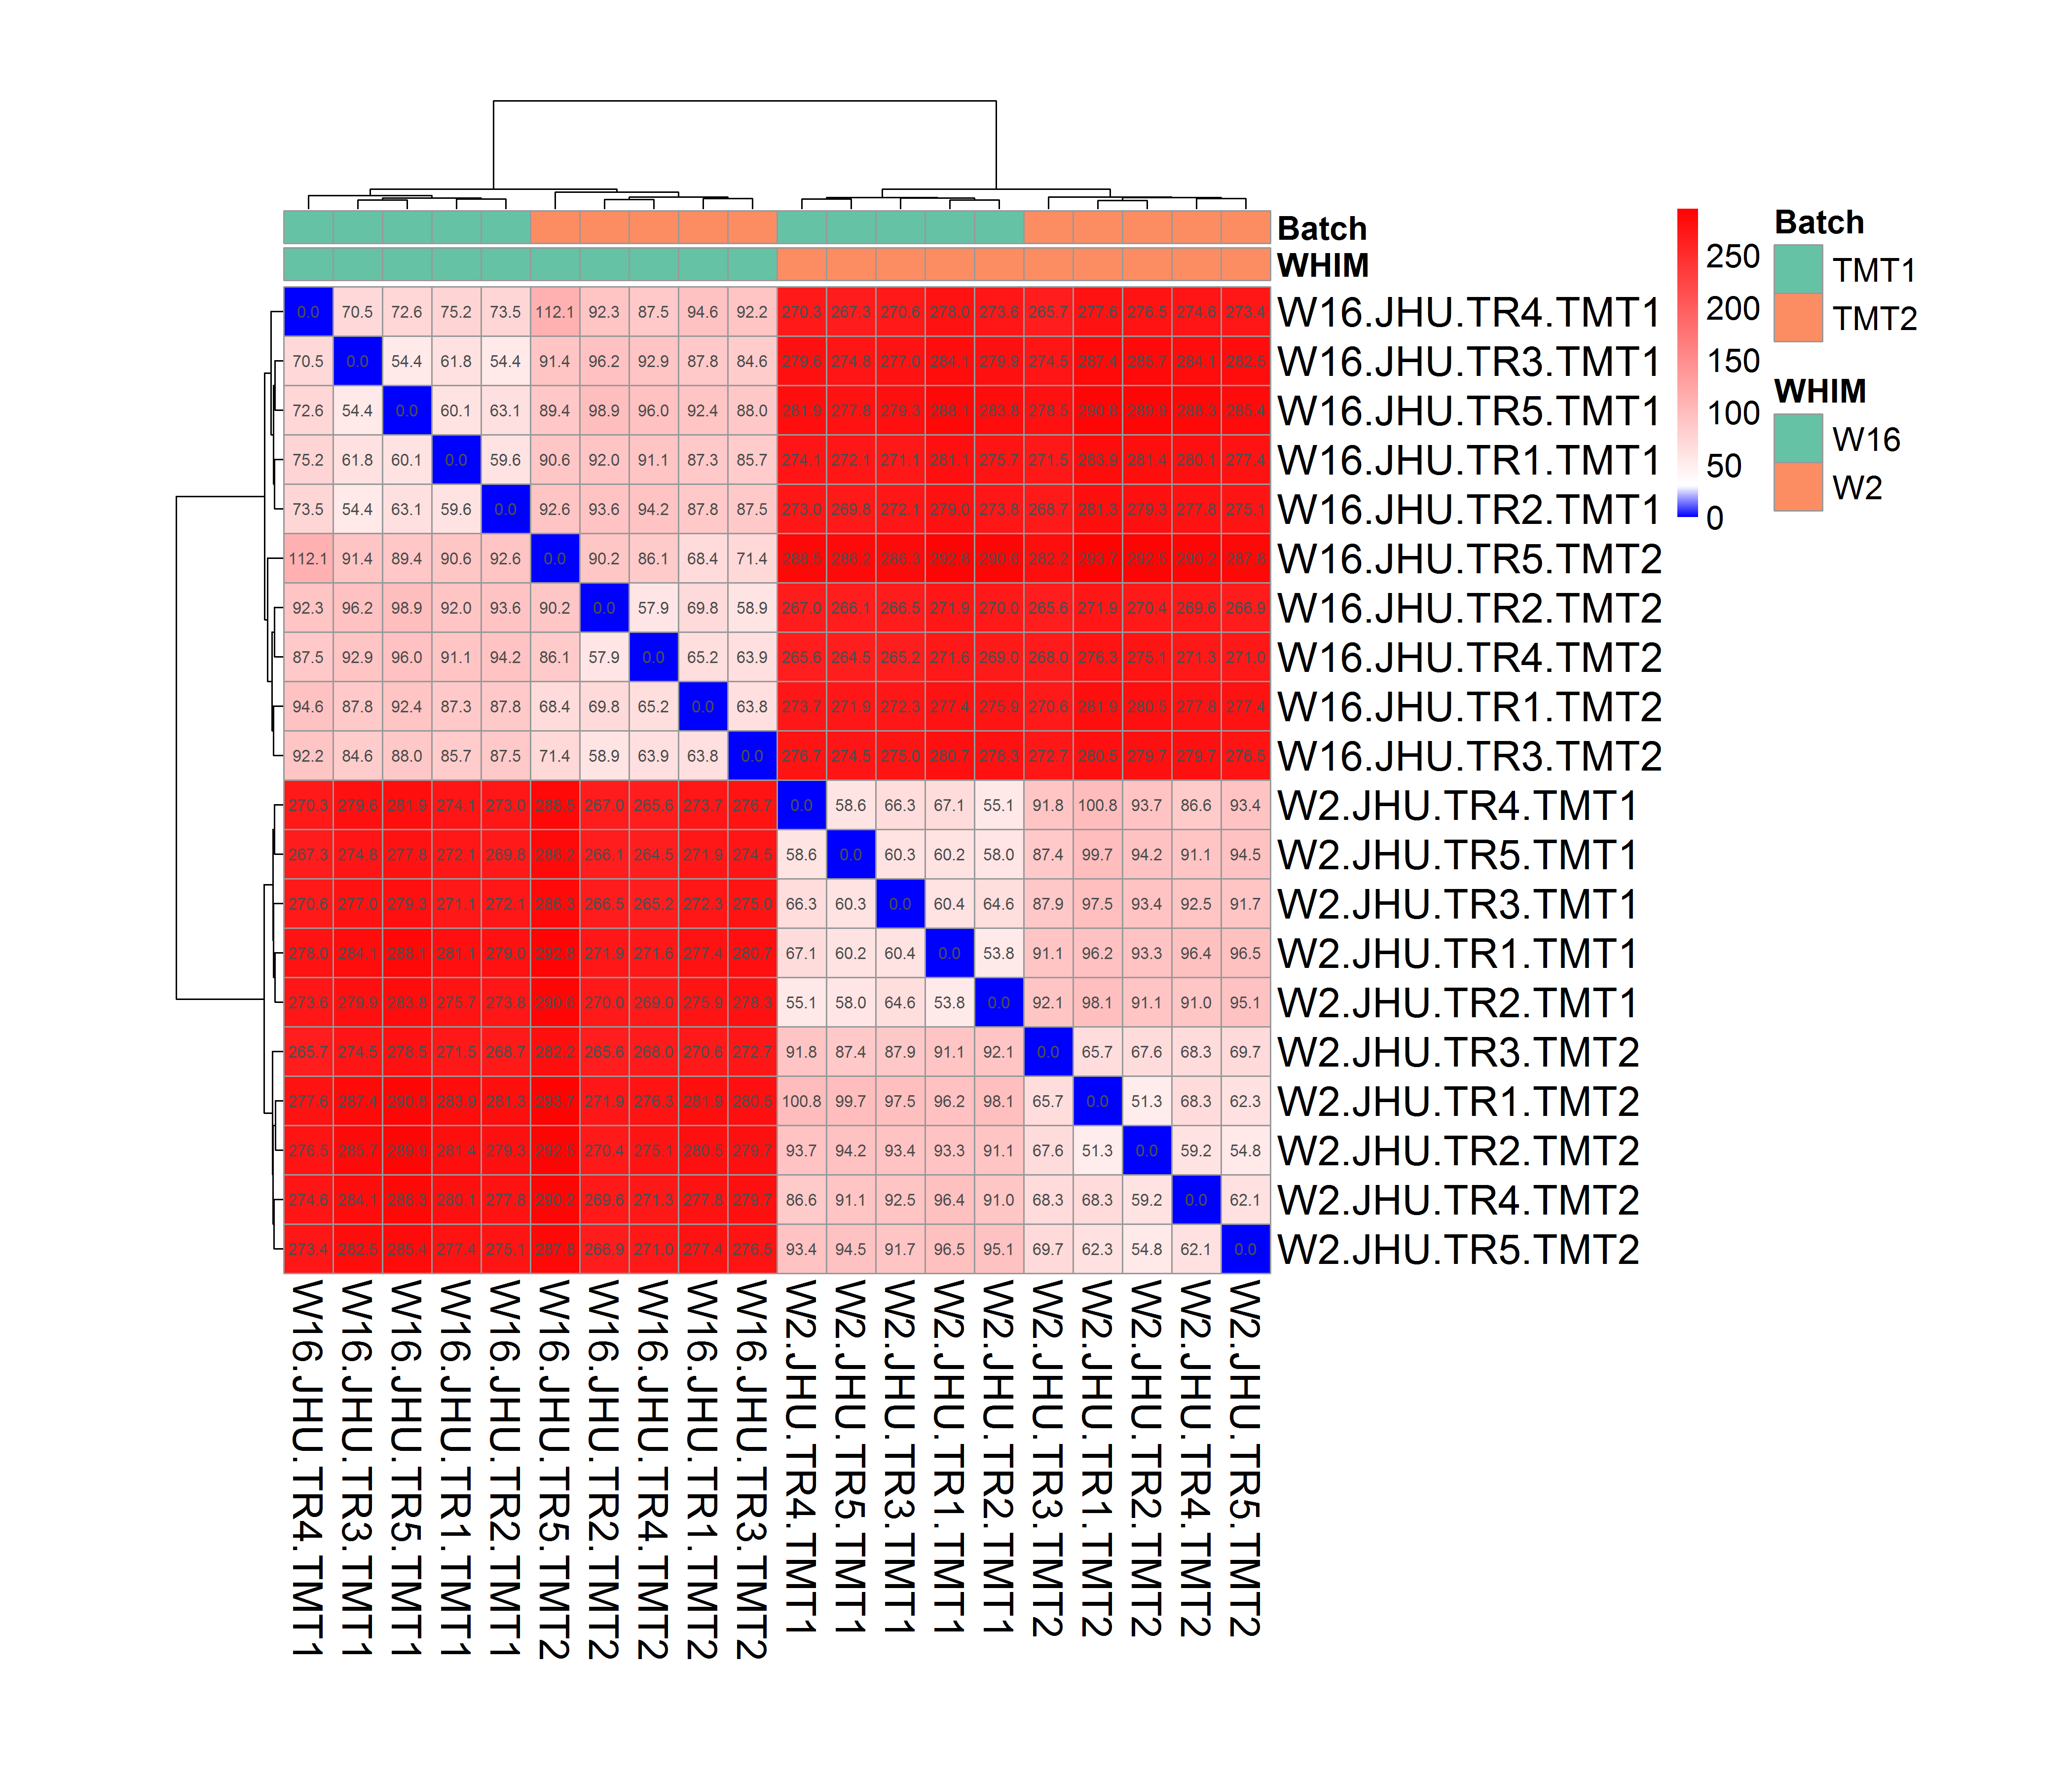
\includegraphics[width=0.45\linewidth]{images\peptide\mds\eucdist_jhu}

\}

\textbackslash{}caption\{\textbf{Figure 2D.} EucDist of peptide log2FC
at \texttt{scale\_log2r\ =\ TRUE}\}\label{fig:Peptide_EucDist}
\textbackslash{}end\{figure\}

\hypertarget{correlation-plots}{%
\subsubsection{Correlation plots}\label{correlation-plots}}

In this section, we visualize the batch effects through correlation
plots. The \texttt{proteoQ} tool currently limits itself to a maximum of
44 samples for a correlation plot. In the demo, we will perform
correlation analysis against the \texttt{PNNL} data subset. By default,
samples will be arranged diagnoally from upper left to bottom right by
the row order of \texttt{expt\_smry.xlsx::Sample\_ID} within a subset.
We have learned from the earlier \texttt{MDS} analysis that the batch
effects are smaller than the differences between \texttt{W2} and
\texttt{W16}. We may wish to put the \texttt{TMT1} and \texttt{TMT2}
groups adjacient to each other for visualization of more nuance batch
effects, followed by the correlational comparison of WHIM subtypes. We
can achieve this by supervising sample IDs at a customized order. In the
\texttt{expt\_smry.xlsx}, I have prepared an \texttt{Order} column where
samples within the \texttt{JHU} subset were arranged in the descending
order of \texttt{W2.TMT1}, \texttt{W2.TMT2}, \texttt{W16.TMT1} and
\texttt{W16.TMT2}. Now we tell the program to look for the
\texttt{Order} column for sample arrangement:

\begin{Shaded}
\begin{Highlighting}[]
\CommentTok{# Correlation plots of peptide data}
\KeywordTok{pepCorr}\NormalTok{(}
    \DataTypeTok{col_select =}\NormalTok{ PNNL,}
    \DataTypeTok{col_order =}\NormalTok{ Order,}
    \DataTypeTok{filename =}\NormalTok{ PNNL.png,}
    
    \DataTypeTok{use_log10 =} \OtherTok{TRUE}\NormalTok{, }
    \DataTypeTok{scale_log2r =} \OtherTok{TRUE}\NormalTok{, }
    \DataTypeTok{min_int =} \FloatTok{3.5}\NormalTok{,}
    \DataTypeTok{max_int =} \FloatTok{6.5}\NormalTok{, }
    \DataTypeTok{min_log2r =} \DecValTok{-2}\NormalTok{, }
    \DataTypeTok{max_log2r =} \DecValTok{2}\NormalTok{, }
    \DataTypeTok{width =} \DecValTok{24}\NormalTok{,}
    \DataTypeTok{height =} \DecValTok{24}
\NormalTok{)}

\CommentTok{# Correlation plots of protein data}
\KeywordTok{prnCorr}\NormalTok{(}
    \DataTypeTok{col_select =}\NormalTok{ PNNL,}
    \DataTypeTok{col_order =}\NormalTok{ Order,}
    \DataTypeTok{filename =}\NormalTok{ PNNL.png,}
    
    \DataTypeTok{use_log10 =} \OtherTok{TRUE}\NormalTok{, }
    \DataTypeTok{scale_log2r =} \OtherTok{TRUE}\NormalTok{, }
    \DataTypeTok{min_int =} \FloatTok{3.5}\NormalTok{,}
    \DataTypeTok{max_int =} \FloatTok{6.5}\NormalTok{, }
    \DataTypeTok{min_log2r =} \DecValTok{-2}\NormalTok{, }
    \DataTypeTok{max_log2r =} \DecValTok{2}\NormalTok{,}
    \DataTypeTok{width =} \DecValTok{24}\NormalTok{,}
    \DataTypeTok{height =} \DecValTok{24}     
\NormalTok{)}
\end{Highlighting}
\end{Shaded}

\begin{figure}

{\centering \includegraphics[width=0.45\linewidth]{images\peptide\corrplot\corr_pnnl} \includegraphics[width=0.45\linewidth]{images\protein\corrplot\corr_pnnl} 

}

\caption{**Figure 3A-3B.** Correlation of log2FC for the `PNNL` subset. Left: peptide; right, protein}\label{fig:Correlation plots}
\end{figure}

More items under construction\ldots{}

The following performs of heat map visualization against protein data:

\begin{Shaded}
\begin{Highlighting}[]
\CommentTok{# Protein heat maps}
\KeywordTok{prnHM}\NormalTok{(}
    \DataTypeTok{xmin =} \DecValTok{-1}\NormalTok{, }
    \DataTypeTok{xmax =} \DecValTok{1}\NormalTok{, }
    \DataTypeTok{x_margin =} \FloatTok{0.1}\NormalTok{, }
    \DataTypeTok{annot_cols =} \KeywordTok{c}\NormalTok{(}\StringTok{"Group"}\NormalTok{, }\StringTok{"Color"}\NormalTok{, }\StringTok{"Alpha"}\NormalTok{, }\StringTok{"Shape"}\NormalTok{), }
    \DataTypeTok{annot_colnames =} \KeywordTok{c}\NormalTok{(}\StringTok{"Group"}\NormalTok{, }\StringTok{"Lab"}\NormalTok{, }\StringTok{"Batch"}\NormalTok{, }\StringTok{"WHIM"}\NormalTok{), }
    \DataTypeTok{cluster_rows =} \OtherTok{TRUE}\NormalTok{, }
    \DataTypeTok{cutree_rows =} \DecValTok{10}\NormalTok{, }
    \DataTypeTok{show_rownames =} \OtherTok{FALSE}\NormalTok{, }
    \DataTypeTok{show_colnames =} \OtherTok{TRUE}\NormalTok{, }
    \DataTypeTok{fontsize_row =} \DecValTok{3}\NormalTok{, }
    \DataTypeTok{cellwidth =} \DecValTok{14}\NormalTok{, }
    \DataTypeTok{width =} \DecValTok{18}\NormalTok{, }
    \DataTypeTok{height =} \DecValTok{12}
\NormalTok{)}
\end{Highlighting}
\end{Shaded}

\textbackslash{}begin\{figure\}

\{\centering 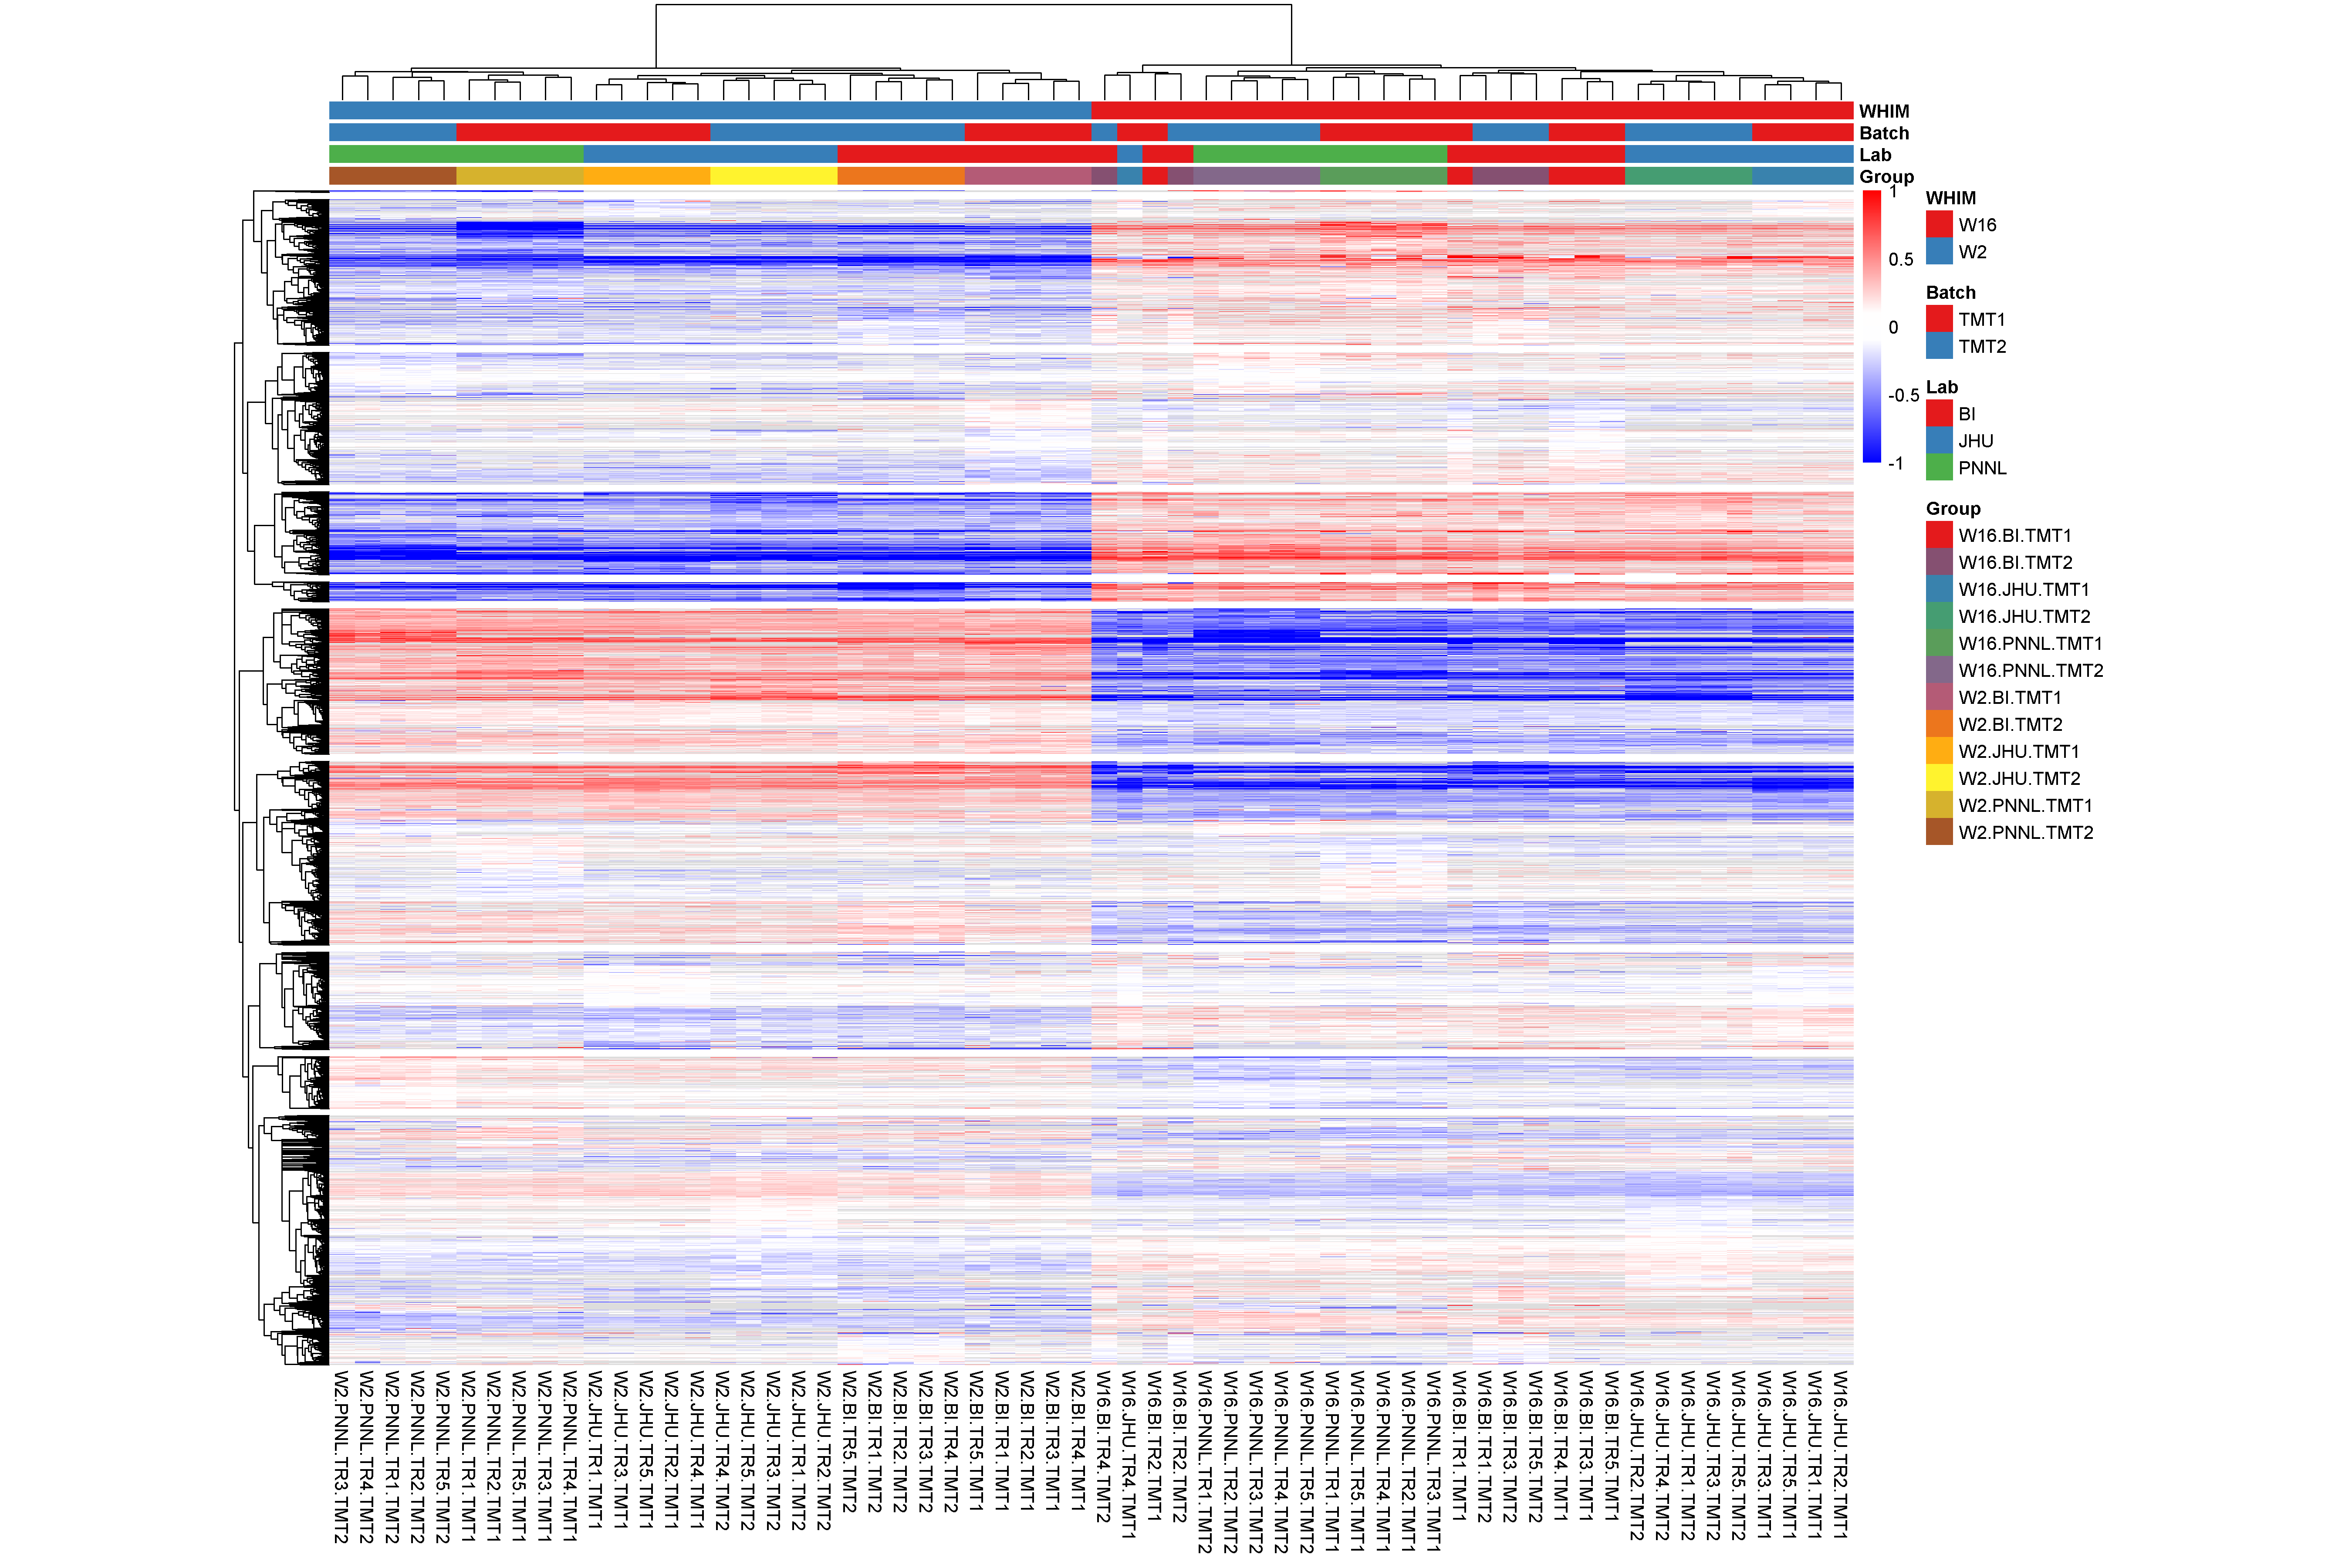
\includegraphics[width=0.8\linewidth]{images\protein\heatmap\heatmap}

\}

\textbackslash{}caption\{\textbf{Figure 4.} Heat map visualization of
protein log2FC at
\texttt{scale\_log2r\ =\ TRUE}\}\label{fig:Protein_heatmap}
\textbackslash{}end\{figure\}

\hypertarget{significance-tests-and-volcano-plot-visualization}{%
\subsubsection{Significance tests and volcano plot
visualization}\label{significance-tests-and-volcano-plot-visualization}}

In this section, we perform the significance analysis of peptide and
protein data. The approach of contrast fit is used in \texttt{proteoQ}
(Chambers, J. M. (1992) Linear models; \texttt{limma}, Gordon Smith). We
first define the contrast groups for significance tests. For this
purpose, I have devided the samples by their WHIM subtypes, laboratory
locations and batch numbers. This ends up with entries of
\texttt{W2.BI.TMT1}, \texttt{W2.BI.TMT2} etc. under the
\texttt{expt\_smry.xlsx::Term} column. The interactive environment
between the Excel file and the proteoQ tool allows us to enter more
columns of contrasts when needed. For instance, we might also be
interested in a more course comparison of inter-laboratory differences
without batch effects. The corresponding contrasts of \texttt{W2.BI},
\texttt{W2.BI} etc. can be found under a pre-made column,
\texttt{Term\_2}. Having these columns in hand, we are now ready to
perform significance tests for peptides and protein species. In the
demo, we will analyze protein data and perform volcano plot
visualization:

\begin{Shaded}
\begin{Highlighting}[]
\CommentTok{# Protein significance tests}
\KeywordTok{prnSig}\NormalTok{(}
    \DataTypeTok{impute_na =} \OtherTok{FALSE}\NormalTok{, }
    \DataTypeTok{W2_bat =} \OperatorTok{~}\StringTok{ }\NormalTok{Term[}\StringTok{"(W2.BI.TMT2-W2.BI.TMT1)"}\NormalTok{, }\StringTok{"(W2.JHU.TMT2-W2.JHU.TMT1)"}\NormalTok{, }\StringTok{"(W2.PNNL.TMT2-W2.PNNL.TMT1)"}\NormalTok{], }\CommentTok{# batch effects}
    \CommentTok{# W2_loc_bat = ~ Term["((W2.BI.TMT1-W2.JHU.TMT1)-(W2.BI.TMT2-W2.JHU.TMT2))", "((W2.BI.TMT1-W2.PNNL.TMT1)-(W2.BI.TMT2-W2.PNNL.TMT2))"], # location and batch effects}
    \DataTypeTok{W2_loc =} \OperatorTok{~}\StringTok{ }\NormalTok{Term_}\DecValTok{2}\NormalTok{[}\StringTok{"W2.BI-W2.JHU"}\NormalTok{, }\StringTok{"W2.BI-W2.PNNL"}\NormalTok{, }\StringTok{"W2.JHU-W2.PNNL"}\NormalTok{] }\CommentTok{# location effects}
\NormalTok{)}

\CommentTok{# Volcano plots}
\KeywordTok{prnVol}\NormalTok{()}
\end{Highlighting}
\end{Shaded}

\begin{verbatim}
Note that we have informed the `prnSig` function to look for contrasts under columns `Term` and `Term_2`, followed by the cotrast pairs in square brackets. Pairs of contrasts are separated by comma.  
\end{verbatim}

Batch effects:

\begin{figure}

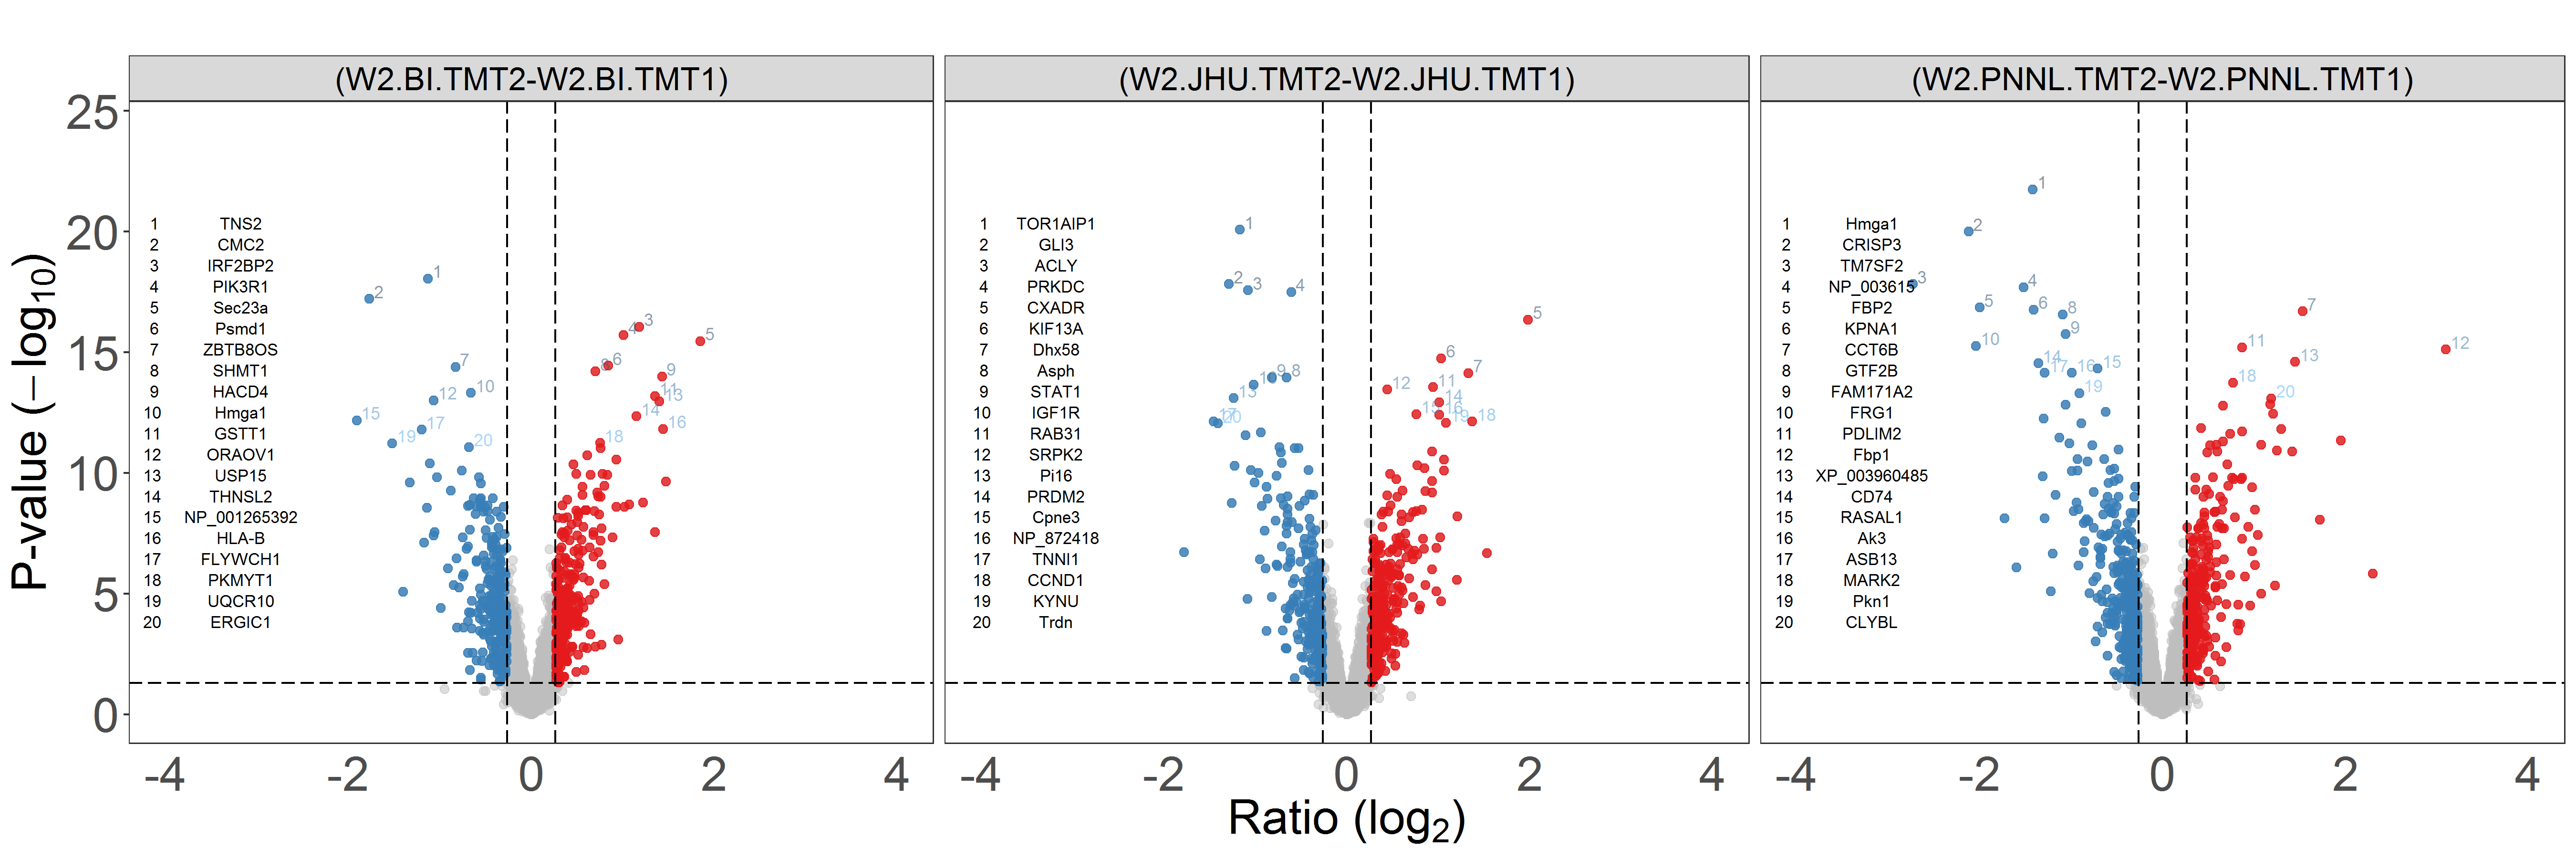
\includegraphics[width=0.8\linewidth]{images\protein\volcplot\batches} \hfill{}

\caption{**Figure 5A.** Volcano plots of protein log2FC between two batches.}\label{fig:Protein_volcano_batches plots}
\end{figure}

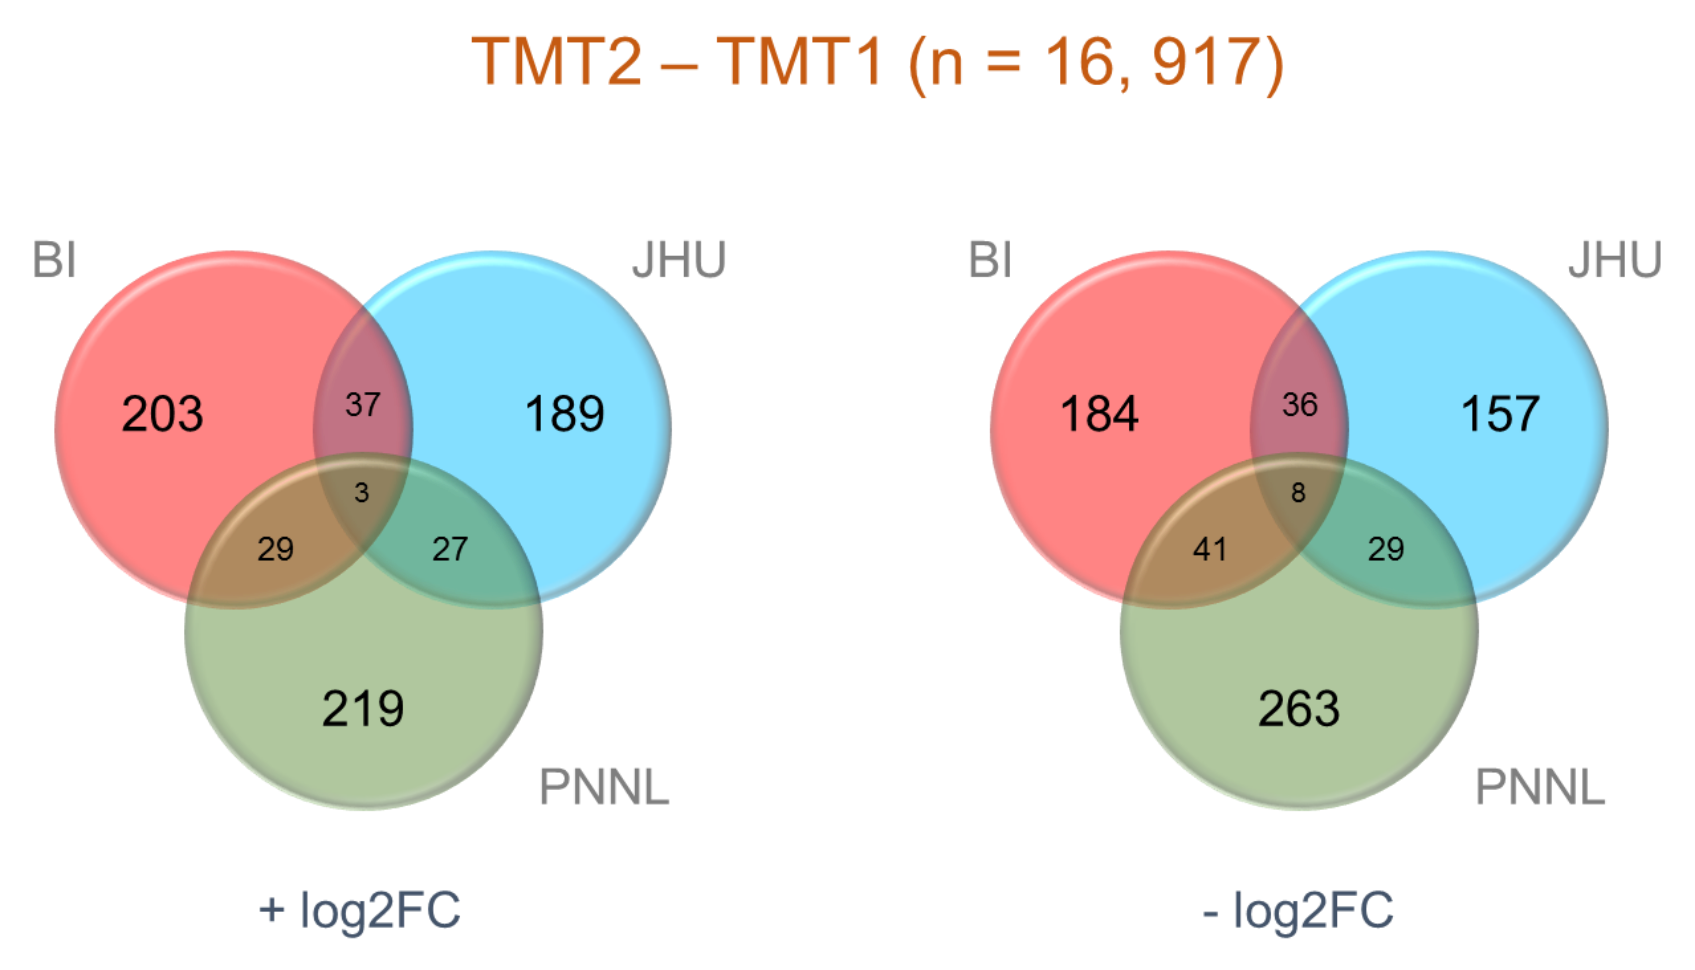
\includegraphics[width=0.8\linewidth]{images\protein\volcplot\venn_batches}

Location effects:

\begin{figure}

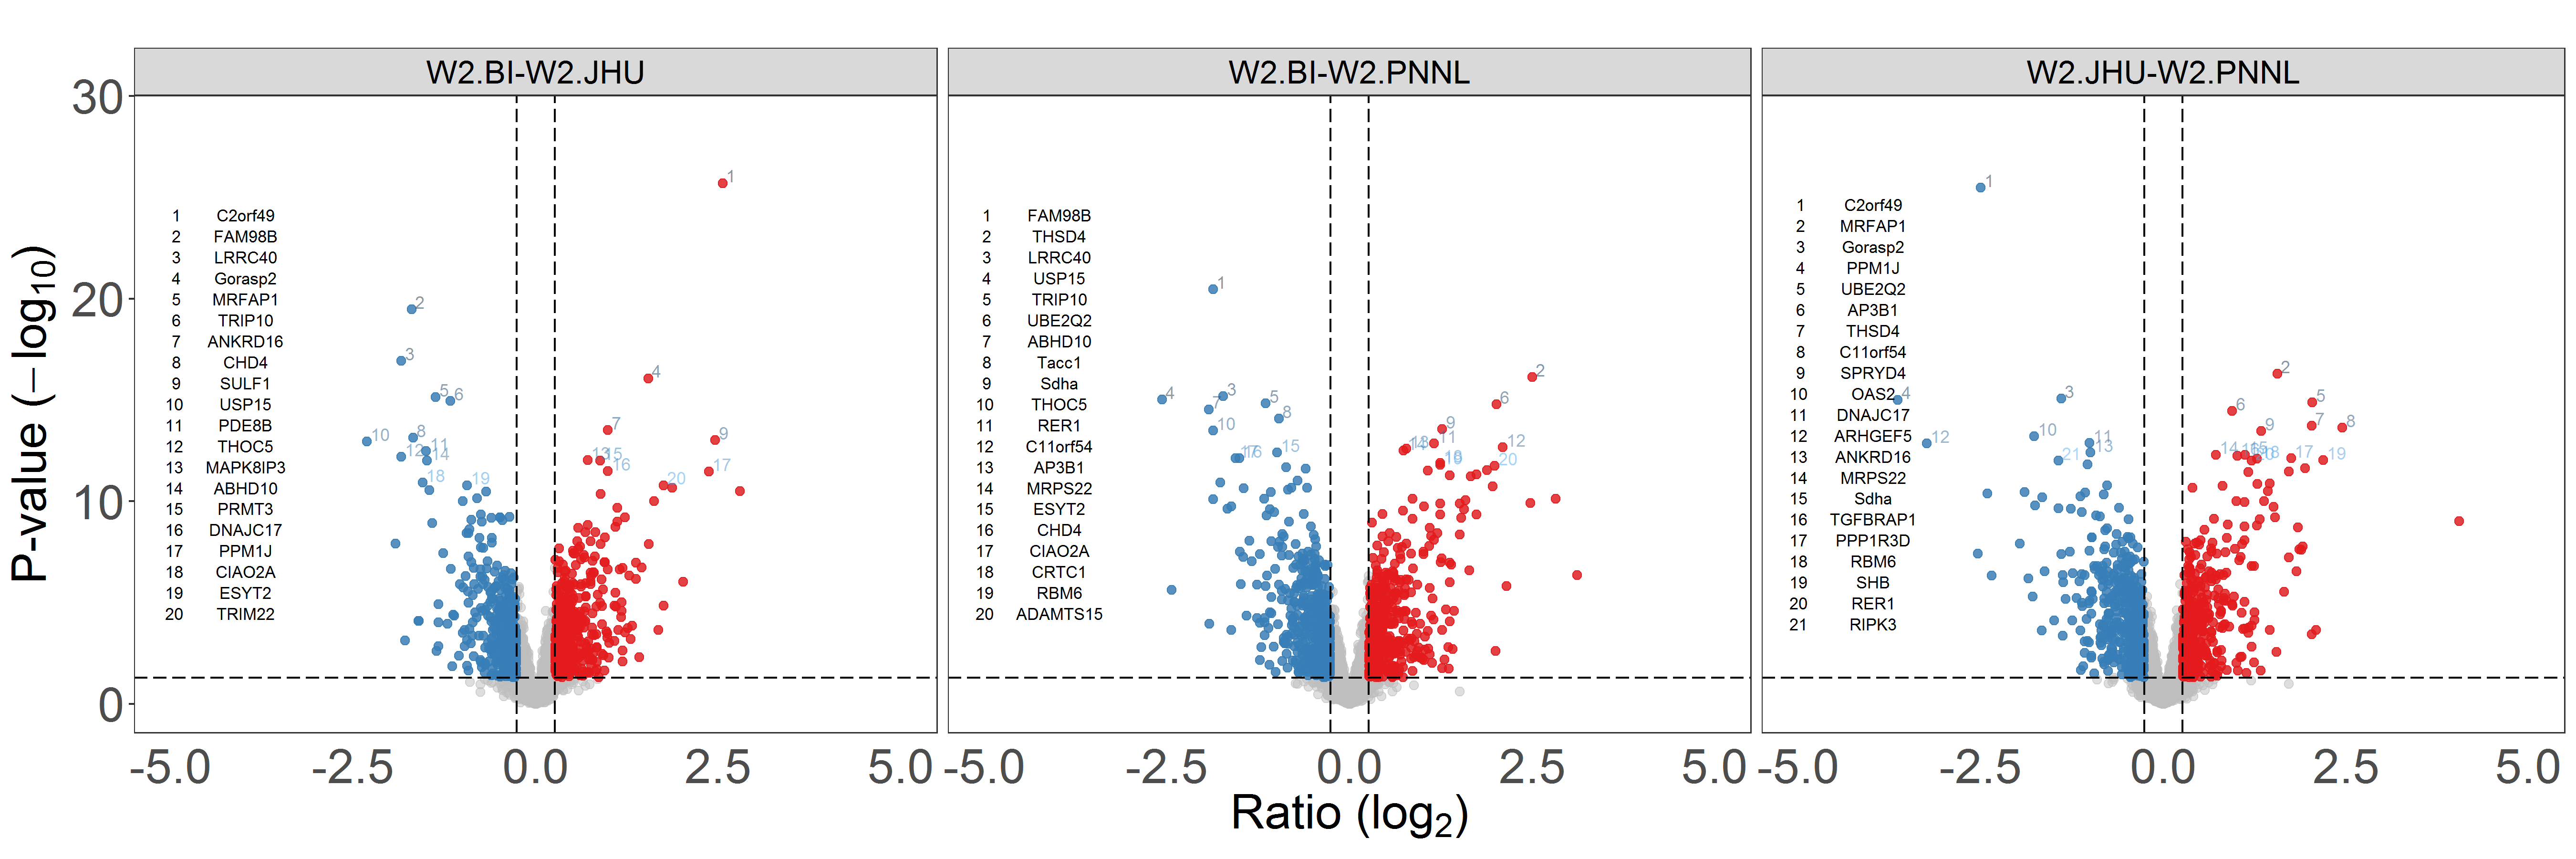
\includegraphics[width=0.8\linewidth]{images\protein\volcplot\locations} \hfill{}

\caption{**Figure 5B.** Volcano plots of protein log2FC between locations.}\label{fig:Protein_volcano_locations plots}
\end{figure}

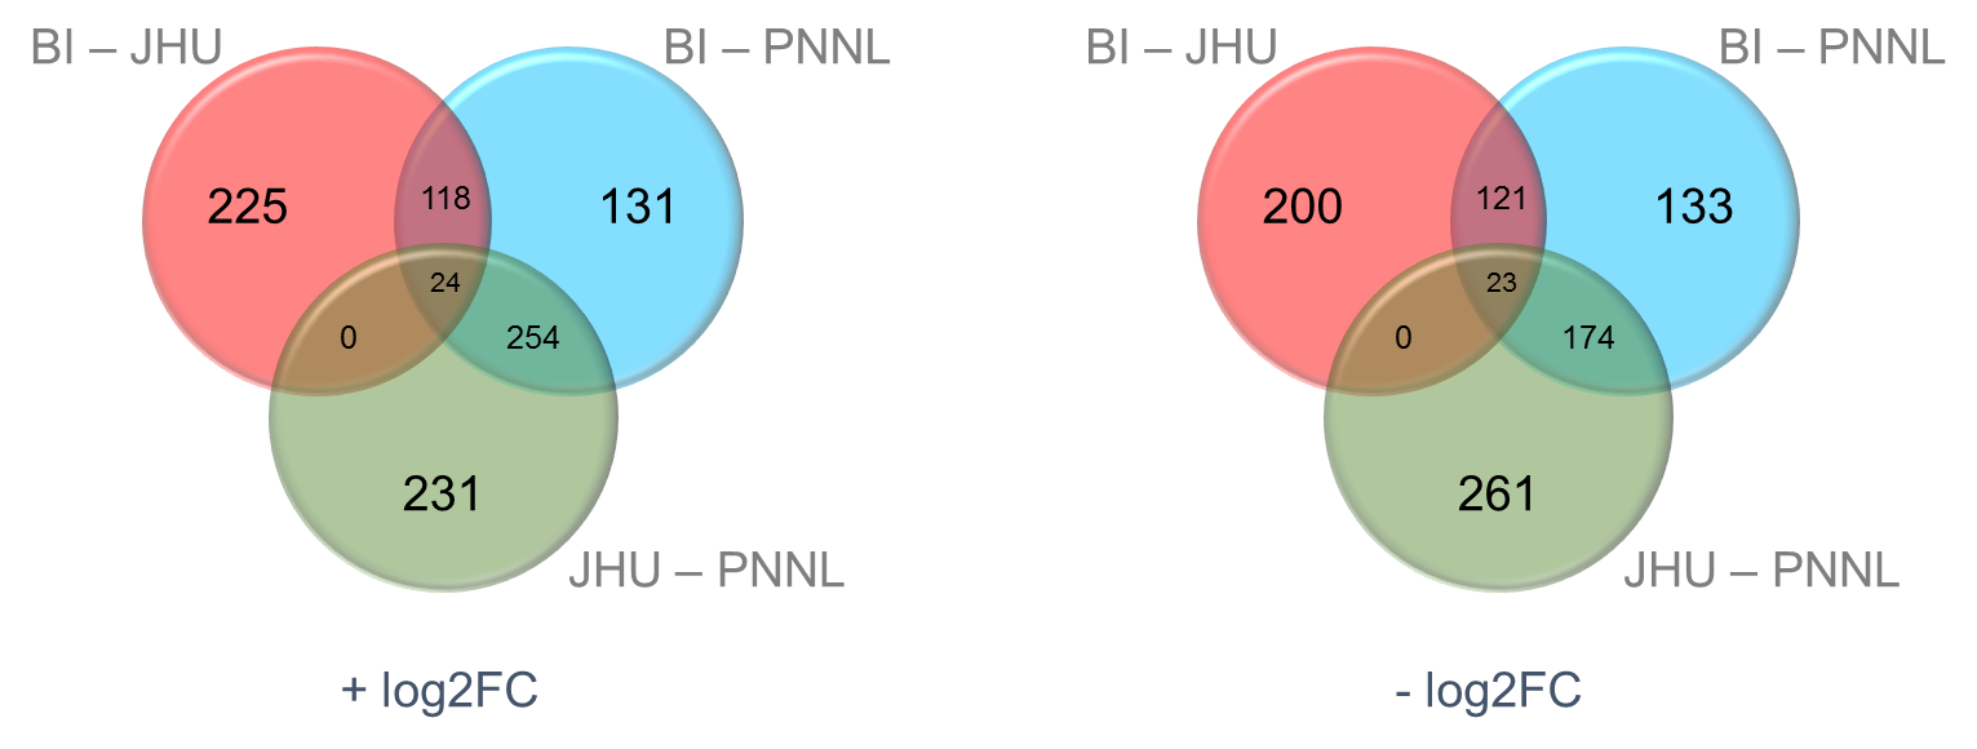
\includegraphics[width=0.8\linewidth]{images\protein\volcplot\venn_locations}

The following performs the imputation of peptide and protein data:

\begin{Shaded}
\begin{Highlighting}[]
\CommentTok{# Impute missing values}
\KeywordTok{pepImp}\NormalTok{(}\DataTypeTok{m =} \DecValTok{2}\NormalTok{, }\DataTypeTok{maxit =} \DecValTok{2}\NormalTok{)}
\KeywordTok{prnImp}\NormalTok{(}\DataTypeTok{m =} \DecValTok{5}\NormalTok{, }\DataTypeTok{maxit =} \DecValTok{5}\NormalTok{)}
\end{Highlighting}
\end{Shaded}

The following performs the trend analysis against protein expressions:

\begin{Shaded}
\begin{Highlighting}[]
\CommentTok{# Soft clustering in protein expressions by trends}
\KeywordTok{anal_prnTrend}\NormalTok{(}
  \DataTypeTok{scale_log2r =} \OtherTok{TRUE}\NormalTok{, }
  \DataTypeTok{n_clust =} \DecValTok{6}
\NormalTok{)}

\CommentTok{# Visualization of trends}
\KeywordTok{plot_prnTrend}\NormalTok{()}
\end{Highlighting}
\end{Shaded}

\begin{figure}

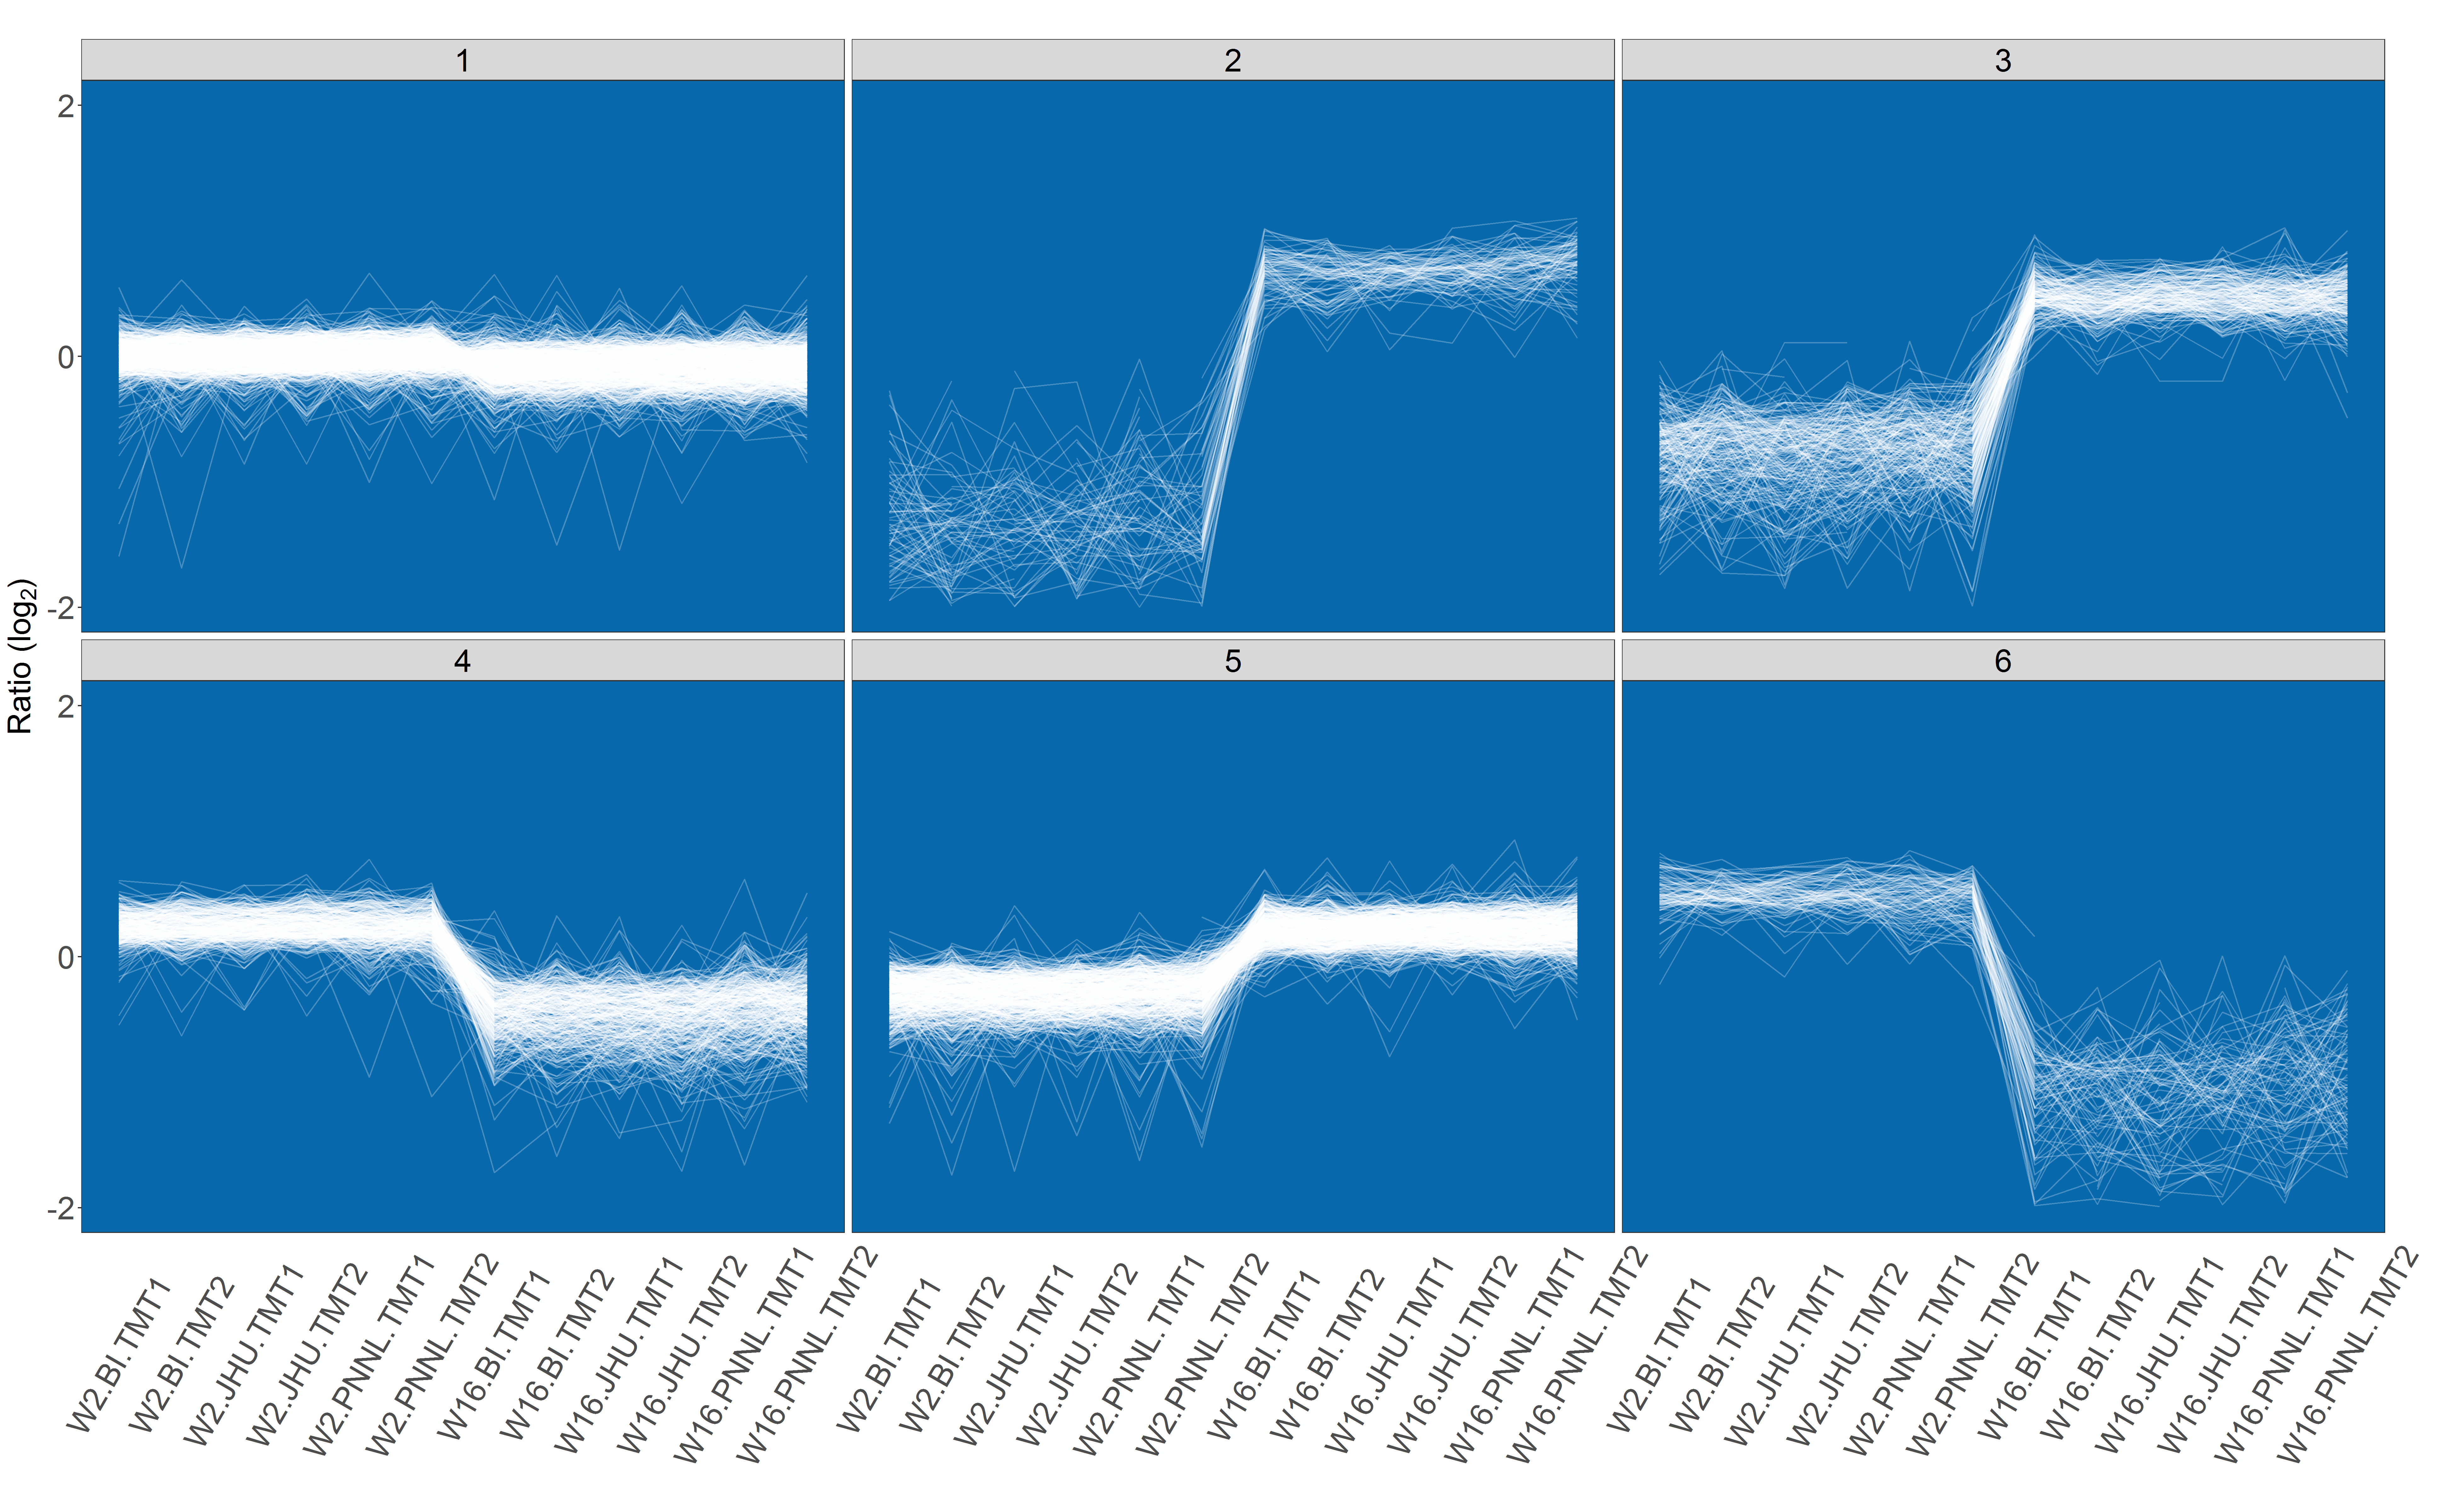
\includegraphics[width=0.8\linewidth]{images\protein\trend\prn_trend_n6} \hfill{}

\caption{**Figure 6.** Trend analysis of protein log2FC.}\label{fig:Protein_trends plots}
\end{figure}

The following performs the NMF analysis against protein data:

\begin{Shaded}
\begin{Highlighting}[]
\CommentTok{# Protein NMF}
\KeywordTok{library}\NormalTok{(NMF)}

\CommentTok{# NMF analysis}
\KeywordTok{anal_prnNMF}\NormalTok{(}
  \CommentTok{# col_group = Group, # optional a priori knowledge of sample groups}
  \DataTypeTok{scale_log2r =} \OtherTok{TRUE}\NormalTok{,}
  \DataTypeTok{r =} \DecValTok{6}\NormalTok{,}
  \DataTypeTok{nrun =} \DecValTok{200}
\NormalTok{)}

\CommentTok{# Consensus heat map}
\KeywordTok{plot_prnNMFCon}\NormalTok{(}
  \DataTypeTok{r =} \DecValTok{6}\NormalTok{, }
  \DataTypeTok{annot_cols =} \KeywordTok{c}\NormalTok{(}\StringTok{"Color"}\NormalTok{, }\StringTok{"Alpha"}\NormalTok{, }\StringTok{"Shape"}\NormalTok{), }
  \DataTypeTok{annot_colnames =} \KeywordTok{c}\NormalTok{(}\StringTok{"Lab"}\NormalTok{, }\StringTok{"Batch"}\NormalTok{, }\StringTok{"WHIM"}\NormalTok{), }
  \DataTypeTok{width =} \DecValTok{10}\NormalTok{, }
  \DataTypeTok{height =} \DecValTok{10}
\NormalTok{)}

\CommentTok{# Coefficient heat map}
\KeywordTok{plot_prnNMFCoef}\NormalTok{(}
  \DataTypeTok{r =} \DecValTok{6}\NormalTok{, }
  \DataTypeTok{annot_cols =} \KeywordTok{c}\NormalTok{(}\StringTok{"Color"}\NormalTok{, }\StringTok{"Alpha"}\NormalTok{, }\StringTok{"Shape"}\NormalTok{), }
  \DataTypeTok{annot_colnames =} \KeywordTok{c}\NormalTok{(}\StringTok{"Lab"}\NormalTok{, }\StringTok{"Batch"}\NormalTok{, }\StringTok{"WHIM"}\NormalTok{), }
  \DataTypeTok{width =} \DecValTok{10}\NormalTok{, }
  \DataTypeTok{height =} \DecValTok{10}
\NormalTok{)}

\CommentTok{# Metagene heat map(s)}
\KeywordTok{plot_metaNMF}\NormalTok{(}
  \DataTypeTok{r =} \DecValTok{6}\NormalTok{, }
  \DataTypeTok{annot_cols =} \KeywordTok{c}\NormalTok{(}\StringTok{"Color"}\NormalTok{, }\StringTok{"Alpha"}\NormalTok{, }\StringTok{"Shape"}\NormalTok{), }
  \DataTypeTok{annot_colnames =} \KeywordTok{c}\NormalTok{(}\StringTok{"Lab"}\NormalTok{, }\StringTok{"Batch"}\NormalTok{, }\StringTok{"WHIM"}\NormalTok{), }
  
  \DataTypeTok{fontsize =} \DecValTok{8}\NormalTok{, }
  \DataTypeTok{fontsize_col =} \DecValTok{5}
\NormalTok{)}
\end{Highlighting}
\end{Shaded}

\begin{figure}

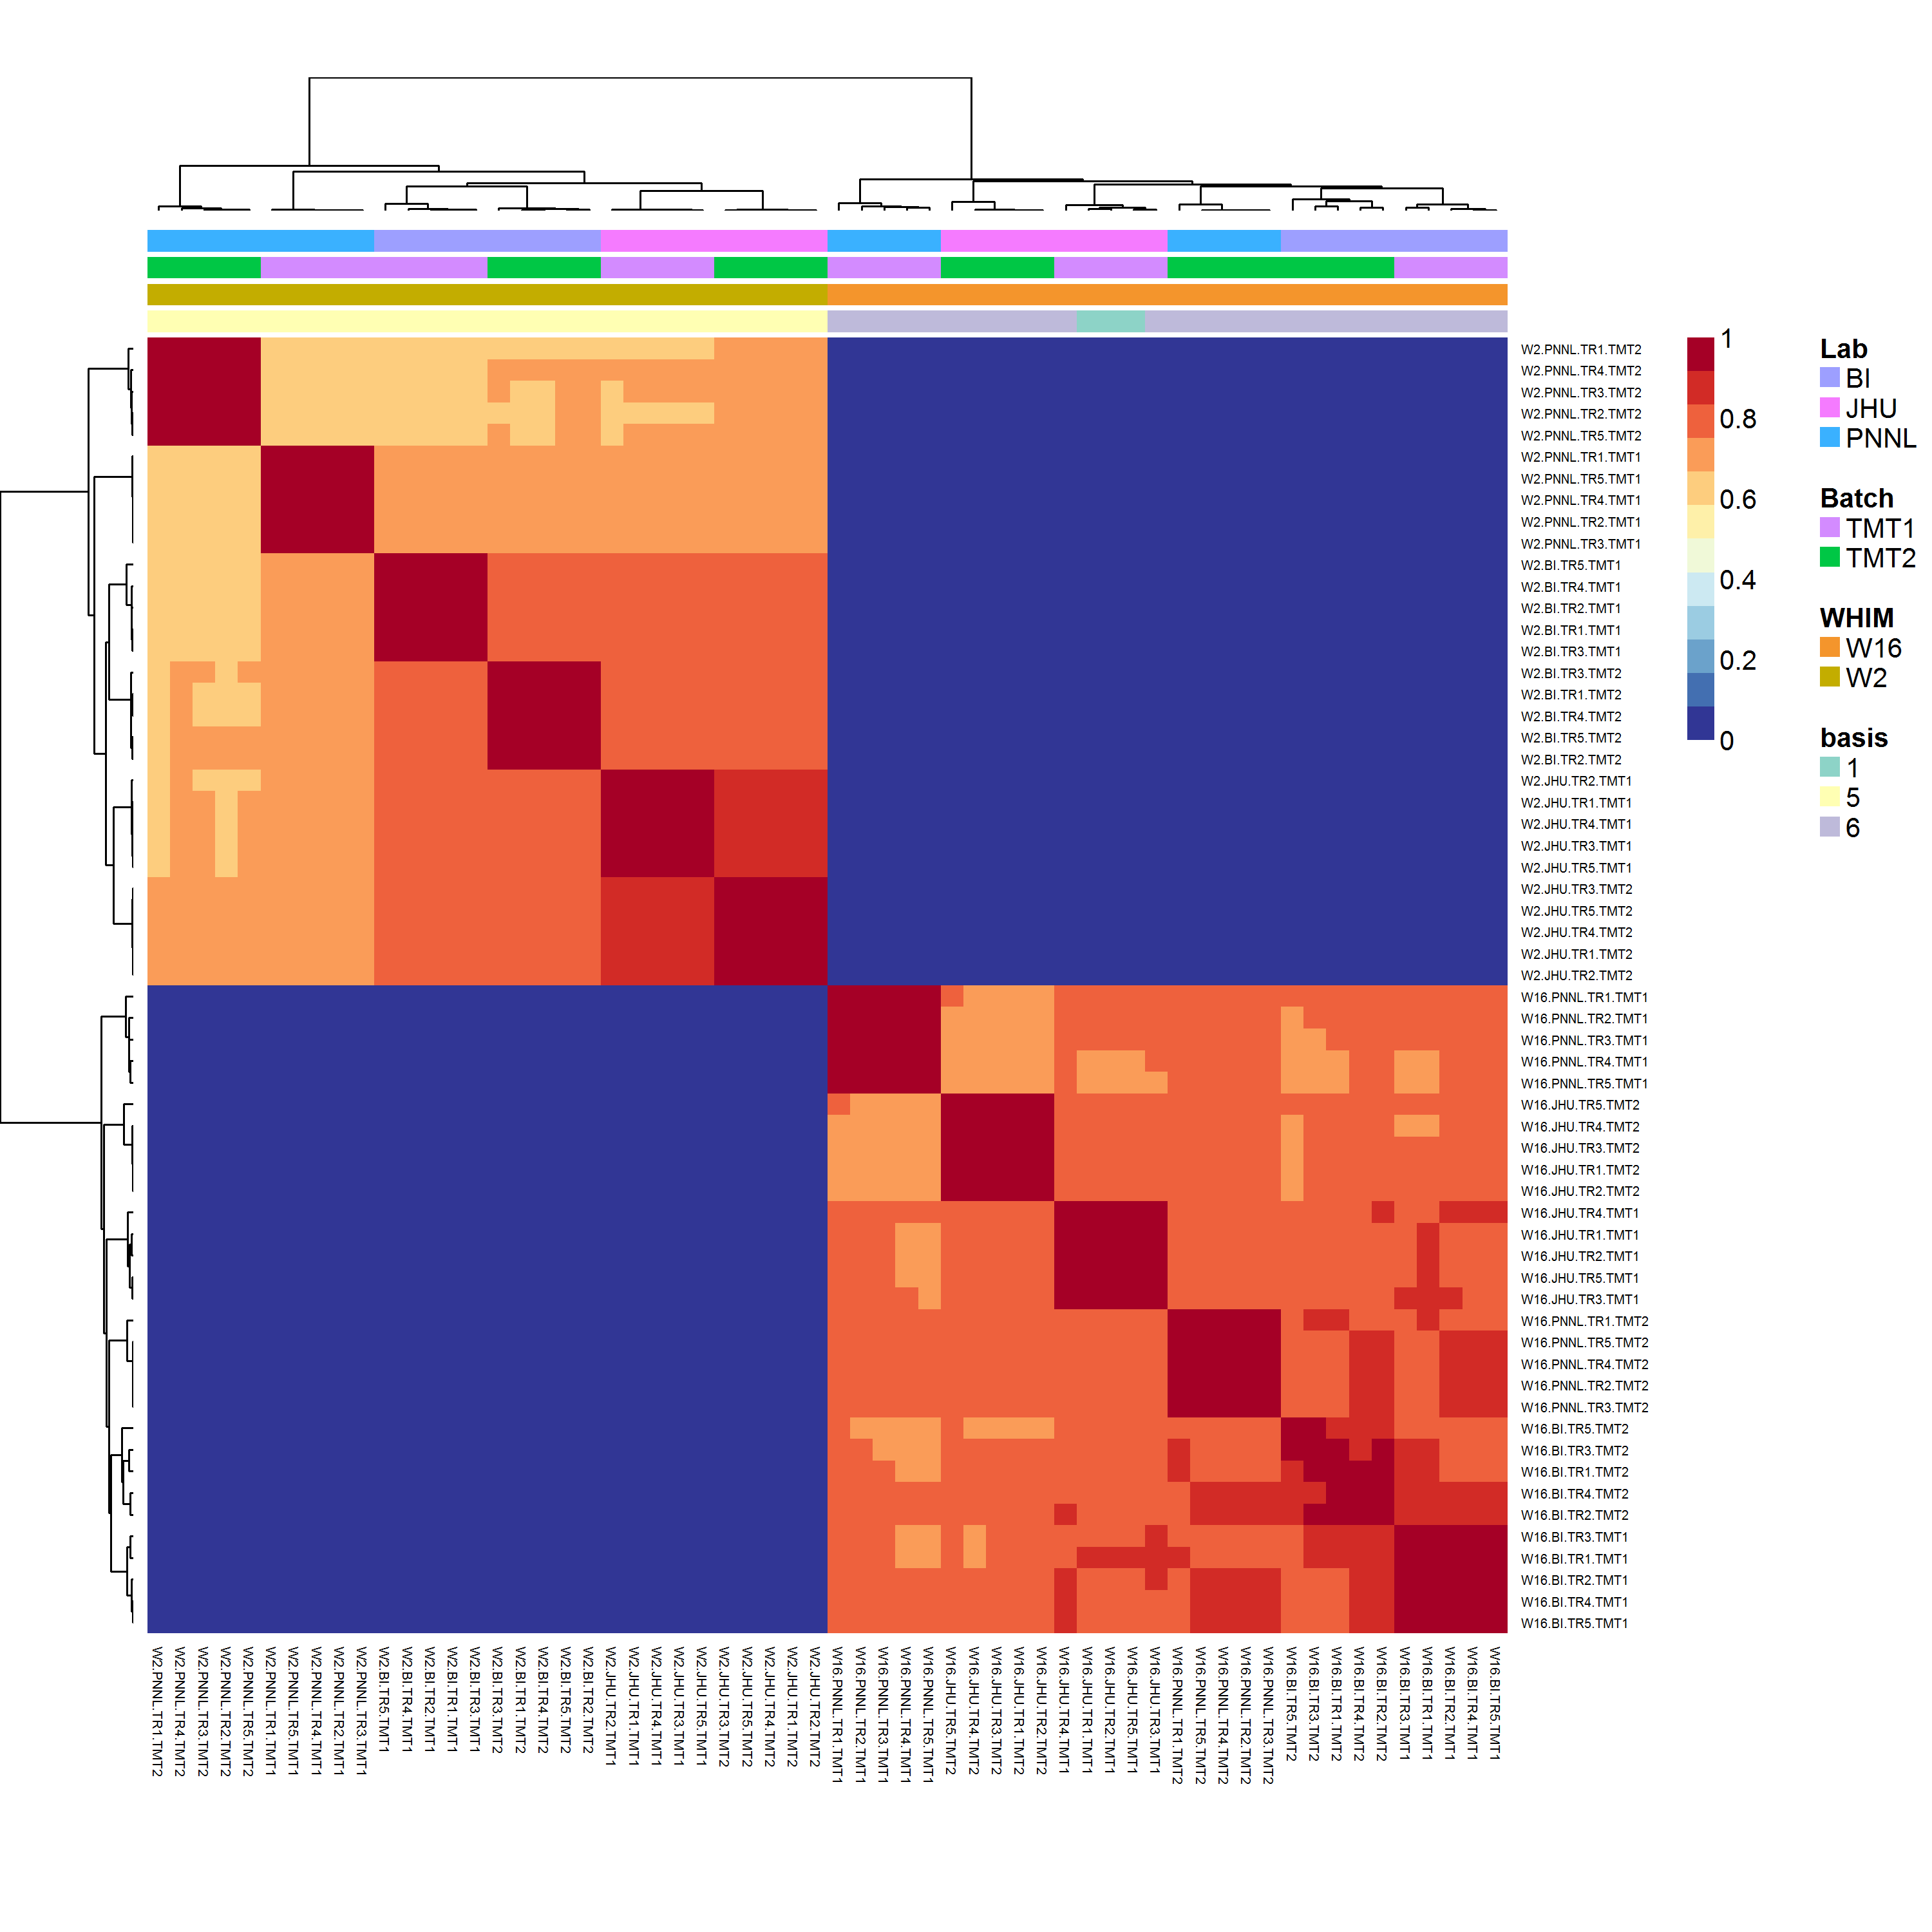
\includegraphics[width=0.45\linewidth]{images\protein\nmf\prn_nmf_r6_consensus} 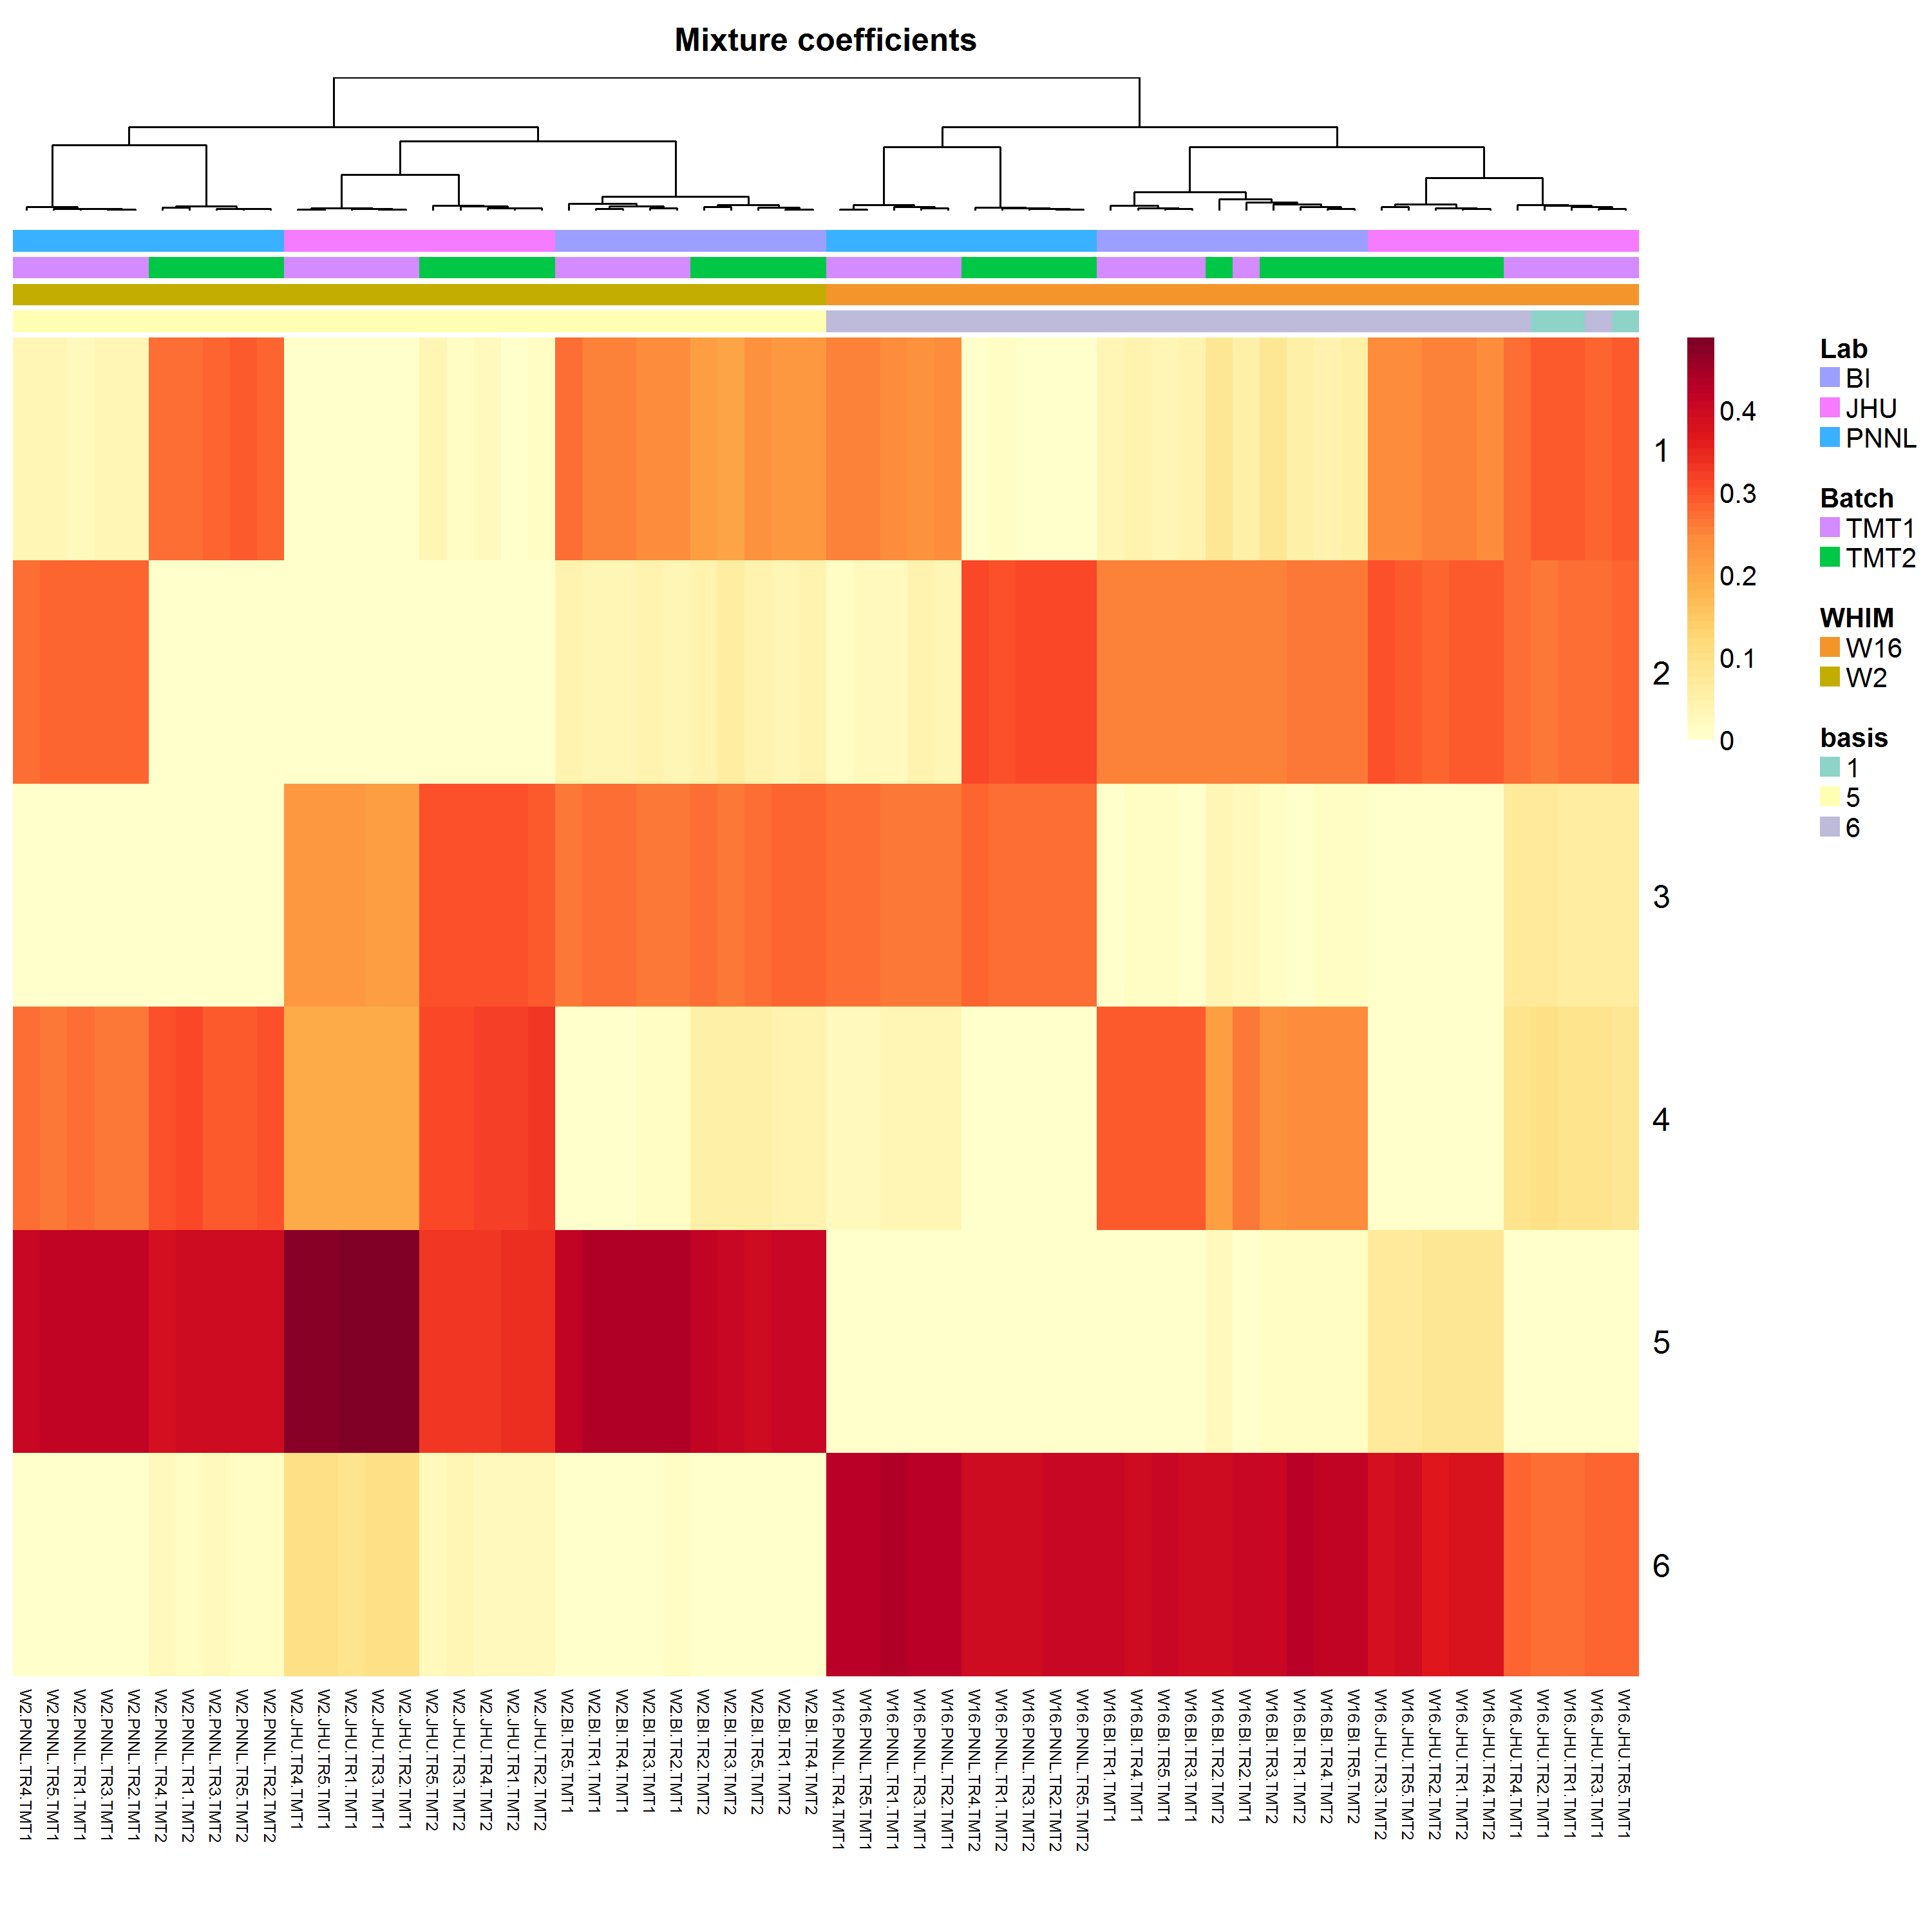
\includegraphics[width=0.45\linewidth]{images\protein\nmf\prn_nmf_r6_coef} \hfill{}

\caption{**Figure 7A-7B.** NMF analysis of protein log2FC. Left: concensus; right: coefficients.}\label{fig:Protein NMF heat maps}
\end{figure}

The following performs GSVA:

\begin{Shaded}
\begin{Highlighting}[]
\KeywordTok{prnGSVA}\NormalTok{(}
  \DataTypeTok{scale_log2r =} \OtherTok{TRUE}\NormalTok{, }
  \DataTypeTok{gset_nm =} \KeywordTok{c}\NormalTok{(}\StringTok{"go_sets"}\NormalTok{, }
              \CommentTok{# "kegg_sets", }
              \StringTok{"c2_msig"}\NormalTok{)}
\NormalTok{)}
\end{Highlighting}
\end{Shaded}

The following maps gene sets under the environment of volcano plot
visualization:

\begin{Shaded}
\begin{Highlighting}[]
\KeywordTok{gsvaMap}\NormalTok{(}
  \DataTypeTok{scale_log2r =} \OtherTok{TRUE}\NormalTok{, }
  \DataTypeTok{pval_cutoff =} \FloatTok{1E-5}\NormalTok{, }
  \DataTypeTok{show_sig =} \StringTok{"pVal"}
\NormalTok{)}
\end{Highlighting}
\end{Shaded}

\hypertarget{lab-choices-of-references}{%
\subsubsection{Lab: Choices of
references}\label{lab-choices-of-references}}

In this lab, we explore the effects of reference choices on data
normalization. We first copy data over to the file directory specified
by \texttt{temp\_dir}, followed by PSM, peptide normalization and
histogram visualization of peptide \texttt{log2FC}.

\begin{Shaded}
\begin{Highlighting}[]
\CommentTok{# directory setup}
\NormalTok{temp_dir <-}\StringTok{ "c:}\CharTok{\textbackslash{}\textbackslash{}}\StringTok{The}\CharTok{\textbackslash{}\textbackslash{}}\StringTok{W2_ref}\CharTok{\textbackslash{}\textbackslash{}}\StringTok{Example"}
\KeywordTok{library}\NormalTok{(proteoQDA)}
\KeywordTok{cptac_csv_1}\NormalTok{(temp_dir)}
\KeywordTok{cptac_expt_ref_w2}\NormalTok{(temp_dir)}
\KeywordTok{cptac_frac_1}\NormalTok{(temp_dir)}

\CommentTok{# analysis}
\KeywordTok{library}\NormalTok{(proteoQ)}
\KeywordTok{load_expts}\NormalTok{(temp_dir, expt_smry_ref_w2.xlsx)}

\KeywordTok{normPSM}\NormalTok{()}

\KeywordTok{normPep}\NormalTok{(}
  \DataTypeTok{id =}\NormalTok{ pep_seq, }
  \DataTypeTok{method_psm_pep =}\NormalTok{ median, }
  \DataTypeTok{method_align =}\NormalTok{ MGKernel, }
  \DataTypeTok{range_log2r =} \KeywordTok{c}\NormalTok{(}\DecValTok{5}\NormalTok{, }\DecValTok{95}\NormalTok{), }
  \DataTypeTok{range_int =} \KeywordTok{c}\NormalTok{(}\DecValTok{5}\NormalTok{, }\DecValTok{95}\NormalTok{), }
  \DataTypeTok{n_comp =} \DecValTok{3}\NormalTok{, }
  \DataTypeTok{seed =} \DecValTok{911}\NormalTok{, }
  \DataTypeTok{maxit =} \DecValTok{200}\NormalTok{, }
  \DataTypeTok{epsilon =} \FloatTok{1e-05}
\NormalTok{)}

\CommentTok{# visualization}
\KeywordTok{pepHist}\NormalTok{(}
    \DataTypeTok{scale_log2r =} \OtherTok{FALSE}\NormalTok{, }
    \DataTypeTok{ncol =} \DecValTok{9}
\NormalTok{)}
\end{Highlighting}
\end{Shaded}

\begin{figure}

{\centering \includegraphics[width=0.8\linewidth]{images\peptide\histogram\peptide_ref_w2} 

}

\caption{**Figure S1A.** Histograms of peptide log2FC with a WHIM2 reference.}\label{fig:Peptide_reference_effect_1}
\end{figure}

Notice that in the above histogram the \texttt{log2FC} profiles of
\texttt{WHIM2} samples are much narrower than those of \texttt{WHIM16}
(\textbf{Figure S1A}). This will occur when a reference is more similar
to one group of sample(s) than the other. In our case, the reference is
one of \texttt{WHIM2}. The difference in the breadth of \texttt{log2FC}
profiles between the \texttt{WHIM16} and the \texttt{WHIM2} groups is
likely due to the genuine difference in their proteomes. If the above
argument is valid, a scaling normalize would moderate, and thus bias,
the quantitative difference in proteomes between \texttt{WHIM2} and
\texttt{WHIM16}.

We alternatively seek a ``center-of-mass'' representation for uses as
references. We select one \texttt{WHIM2} and one \texttt{WHIM16} from
each 10-plex TMT. The \texttt{proteoQ} tool will average the signals
from designated references. Thefore, the derived reference can be viewed
as a mid point of the \texttt{WHIM2} and the \texttt{WHIM16} proteomes.
We next perform analogously the data summary and histogram
visualization. With the new reference, we have achieved \texttt{log2FC}
profiles that are more comparable in breadth between \texttt{WHIM2} and
\texttt{WHIM16} samples. With the new reference, a scaling normalization
may be suitable at later steps.

\begin{Shaded}
\begin{Highlighting}[]
\CommentTok{# directory setup}
\NormalTok{temp_dir_}\DecValTok{2}\NormalTok{ <-}\StringTok{ "c:}\CharTok{\textbackslash{}\textbackslash{}}\StringTok{The}\CharTok{\textbackslash{}\textbackslash{}}\StringTok{W2_W16_ref}\CharTok{\textbackslash{}\textbackslash{}}\StringTok{Example"}
\KeywordTok{library}\NormalTok{(proteoQDA)}
\KeywordTok{cptac_csv_1}\NormalTok{(temp_dir_}\DecValTok{2}\NormalTok{)}
\KeywordTok{expt_smry_ref_w2_w16}\NormalTok{(temp_dir_}\DecValTok{2}\NormalTok{)}
\KeywordTok{cptac_frac_1}\NormalTok{(temp_dir_}\DecValTok{2}\NormalTok{)}

\CommentTok{# analysis}
\KeywordTok{library}\NormalTok{(proteoQ)}
\KeywordTok{load_expts}\NormalTok{(temp_dir_}\DecValTok{2}\NormalTok{, expt_smry_ref_w2_w16.xlsx)}

\KeywordTok{normPSM}\NormalTok{()}

\KeywordTok{normPep}\NormalTok{(}
  \DataTypeTok{id =}\NormalTok{ pep_seq, }
  \DataTypeTok{method_psm_pep =}\NormalTok{ median, }
  \DataTypeTok{method_align =}\NormalTok{ MGKernel, }
  \DataTypeTok{range_log2r =} \KeywordTok{c}\NormalTok{(}\DecValTok{5}\NormalTok{, }\DecValTok{95}\NormalTok{), }
  \DataTypeTok{range_int =} \KeywordTok{c}\NormalTok{(}\DecValTok{5}\NormalTok{, }\DecValTok{95}\NormalTok{), }
  \DataTypeTok{n_comp =} \DecValTok{3}\NormalTok{, }
  \DataTypeTok{seed =} \DecValTok{911}\NormalTok{, }
  \DataTypeTok{maxit =} \DecValTok{200}\NormalTok{, }
  \DataTypeTok{epsilon =} \FloatTok{1e-05}
\NormalTok{)}

\CommentTok{# visualization}
\KeywordTok{pepHist}\NormalTok{(}
    \DataTypeTok{scale_log2r =} \OtherTok{FALSE}\NormalTok{, }
    \DataTypeTok{ncol =} \DecValTok{8}
\NormalTok{)}
\end{Highlighting}
\end{Shaded}

\begin{figure}

{\centering \includegraphics[width=0.8\linewidth]{images\peptide\histogram\peptide_ref_w2_w16} 

}

\caption{**Figure S1B.** Histograms of peptide log2FC with a combined WHIM2 and WHIM16 reference.}\label{fig:Peptide_reference_effect_2}
\end{figure}

\hypertarget{lab-peptide-subsets}{%
\subsubsection{Lab: Peptide subsets}\label{lab-peptide-subsets}}

In addition to the global proteomes, the CPTAC publication contains
phosphopeptide data from the same samples.(2018) In this lab, we will
explore the stoichiometry of phosphopeptide subsets in relative to the
combined data sets of \texttt{global\ +\ phospho} peptides. We first
performed a search aganist the combined \texttt{global\ and\ phospho}
data. The search results are available in \texttt{proteoQDA}. We next
copy the result files over, followed by the analysis and visualization
of the \texttt{BI} subset:

\begin{Shaded}
\begin{Highlighting}[]
\CommentTok{# directory setup}
\NormalTok{temp_phospho_dir <-}\StringTok{ "c:}\CharTok{\textbackslash{}\textbackslash{}}\StringTok{The}\CharTok{\textbackslash{}\textbackslash{}}\StringTok{Phosphopeptide}\CharTok{\textbackslash{}\textbackslash{}}\StringTok{Example"}
\KeywordTok{library}\NormalTok{(proteoQDA)}
\KeywordTok{cptac_csv_2}\NormalTok{(temp_phospho_dir)}
\KeywordTok{cptac_expt_2}\NormalTok{(temp_phospho_dir)}
\KeywordTok{cptac_frac_2}\NormalTok{(temp_phospho_dir)}

\CommentTok{# analysis}
\KeywordTok{library}\NormalTok{(proteoQ)}
\KeywordTok{load_expts}\NormalTok{(temp_phospho_dir, expt_smry.xlsx)}

\KeywordTok{normPSM}\NormalTok{()}

\KeywordTok{normPep}\NormalTok{(}
  \DataTypeTok{id =}\NormalTok{ pep_seq_mod, }\CommentTok{# peptides with different variable modifications}
  \DataTypeTok{method_psm_pep =}\NormalTok{ median, }
  \DataTypeTok{method_align =}\NormalTok{ MGKernel, }
  \DataTypeTok{range_log2r =} \KeywordTok{c}\NormalTok{(}\DecValTok{5}\NormalTok{, }\DecValTok{95}\NormalTok{), }
  \DataTypeTok{range_int =} \KeywordTok{c}\NormalTok{(}\DecValTok{5}\NormalTok{, }\DecValTok{95}\NormalTok{), }
  \DataTypeTok{n_comp =} \DecValTok{3}\NormalTok{, }
  \DataTypeTok{seed =} \DecValTok{749662}\NormalTok{, }
  \DataTypeTok{maxit =} \DecValTok{200}\NormalTok{, }
  \DataTypeTok{epsilon =} \FloatTok{1e-05}
\NormalTok{)}

\CommentTok{# all peptides}
\KeywordTok{pepHist}\NormalTok{(}
    \DataTypeTok{col_select =}\NormalTok{ BI, }
    \DataTypeTok{scale_log2r =} \OtherTok{TRUE}\NormalTok{, }
    \DataTypeTok{ncol =} \DecValTok{4}\NormalTok{, }
    \DataTypeTok{filename =} \StringTok{"BI_all_peptides.png"}
\NormalTok{)}

\CommentTok{# phospho subsets}
\KeywordTok{pepHist}\NormalTok{(}
    \DataTypeTok{col_select =}\NormalTok{ BI, }
    \DataTypeTok{scale_log2r =} \OtherTok{TRUE}\NormalTok{, }
    \DataTypeTok{pep_pattern =} \StringTok{"sty"}\NormalTok{, }
    \DataTypeTok{ncol =} \DecValTok{4}\NormalTok{, }
    \DataTypeTok{filename =} \StringTok{"BI_pSTY.png"}
\NormalTok{)}
\end{Highlighting}
\end{Shaded}

\begin{figure}

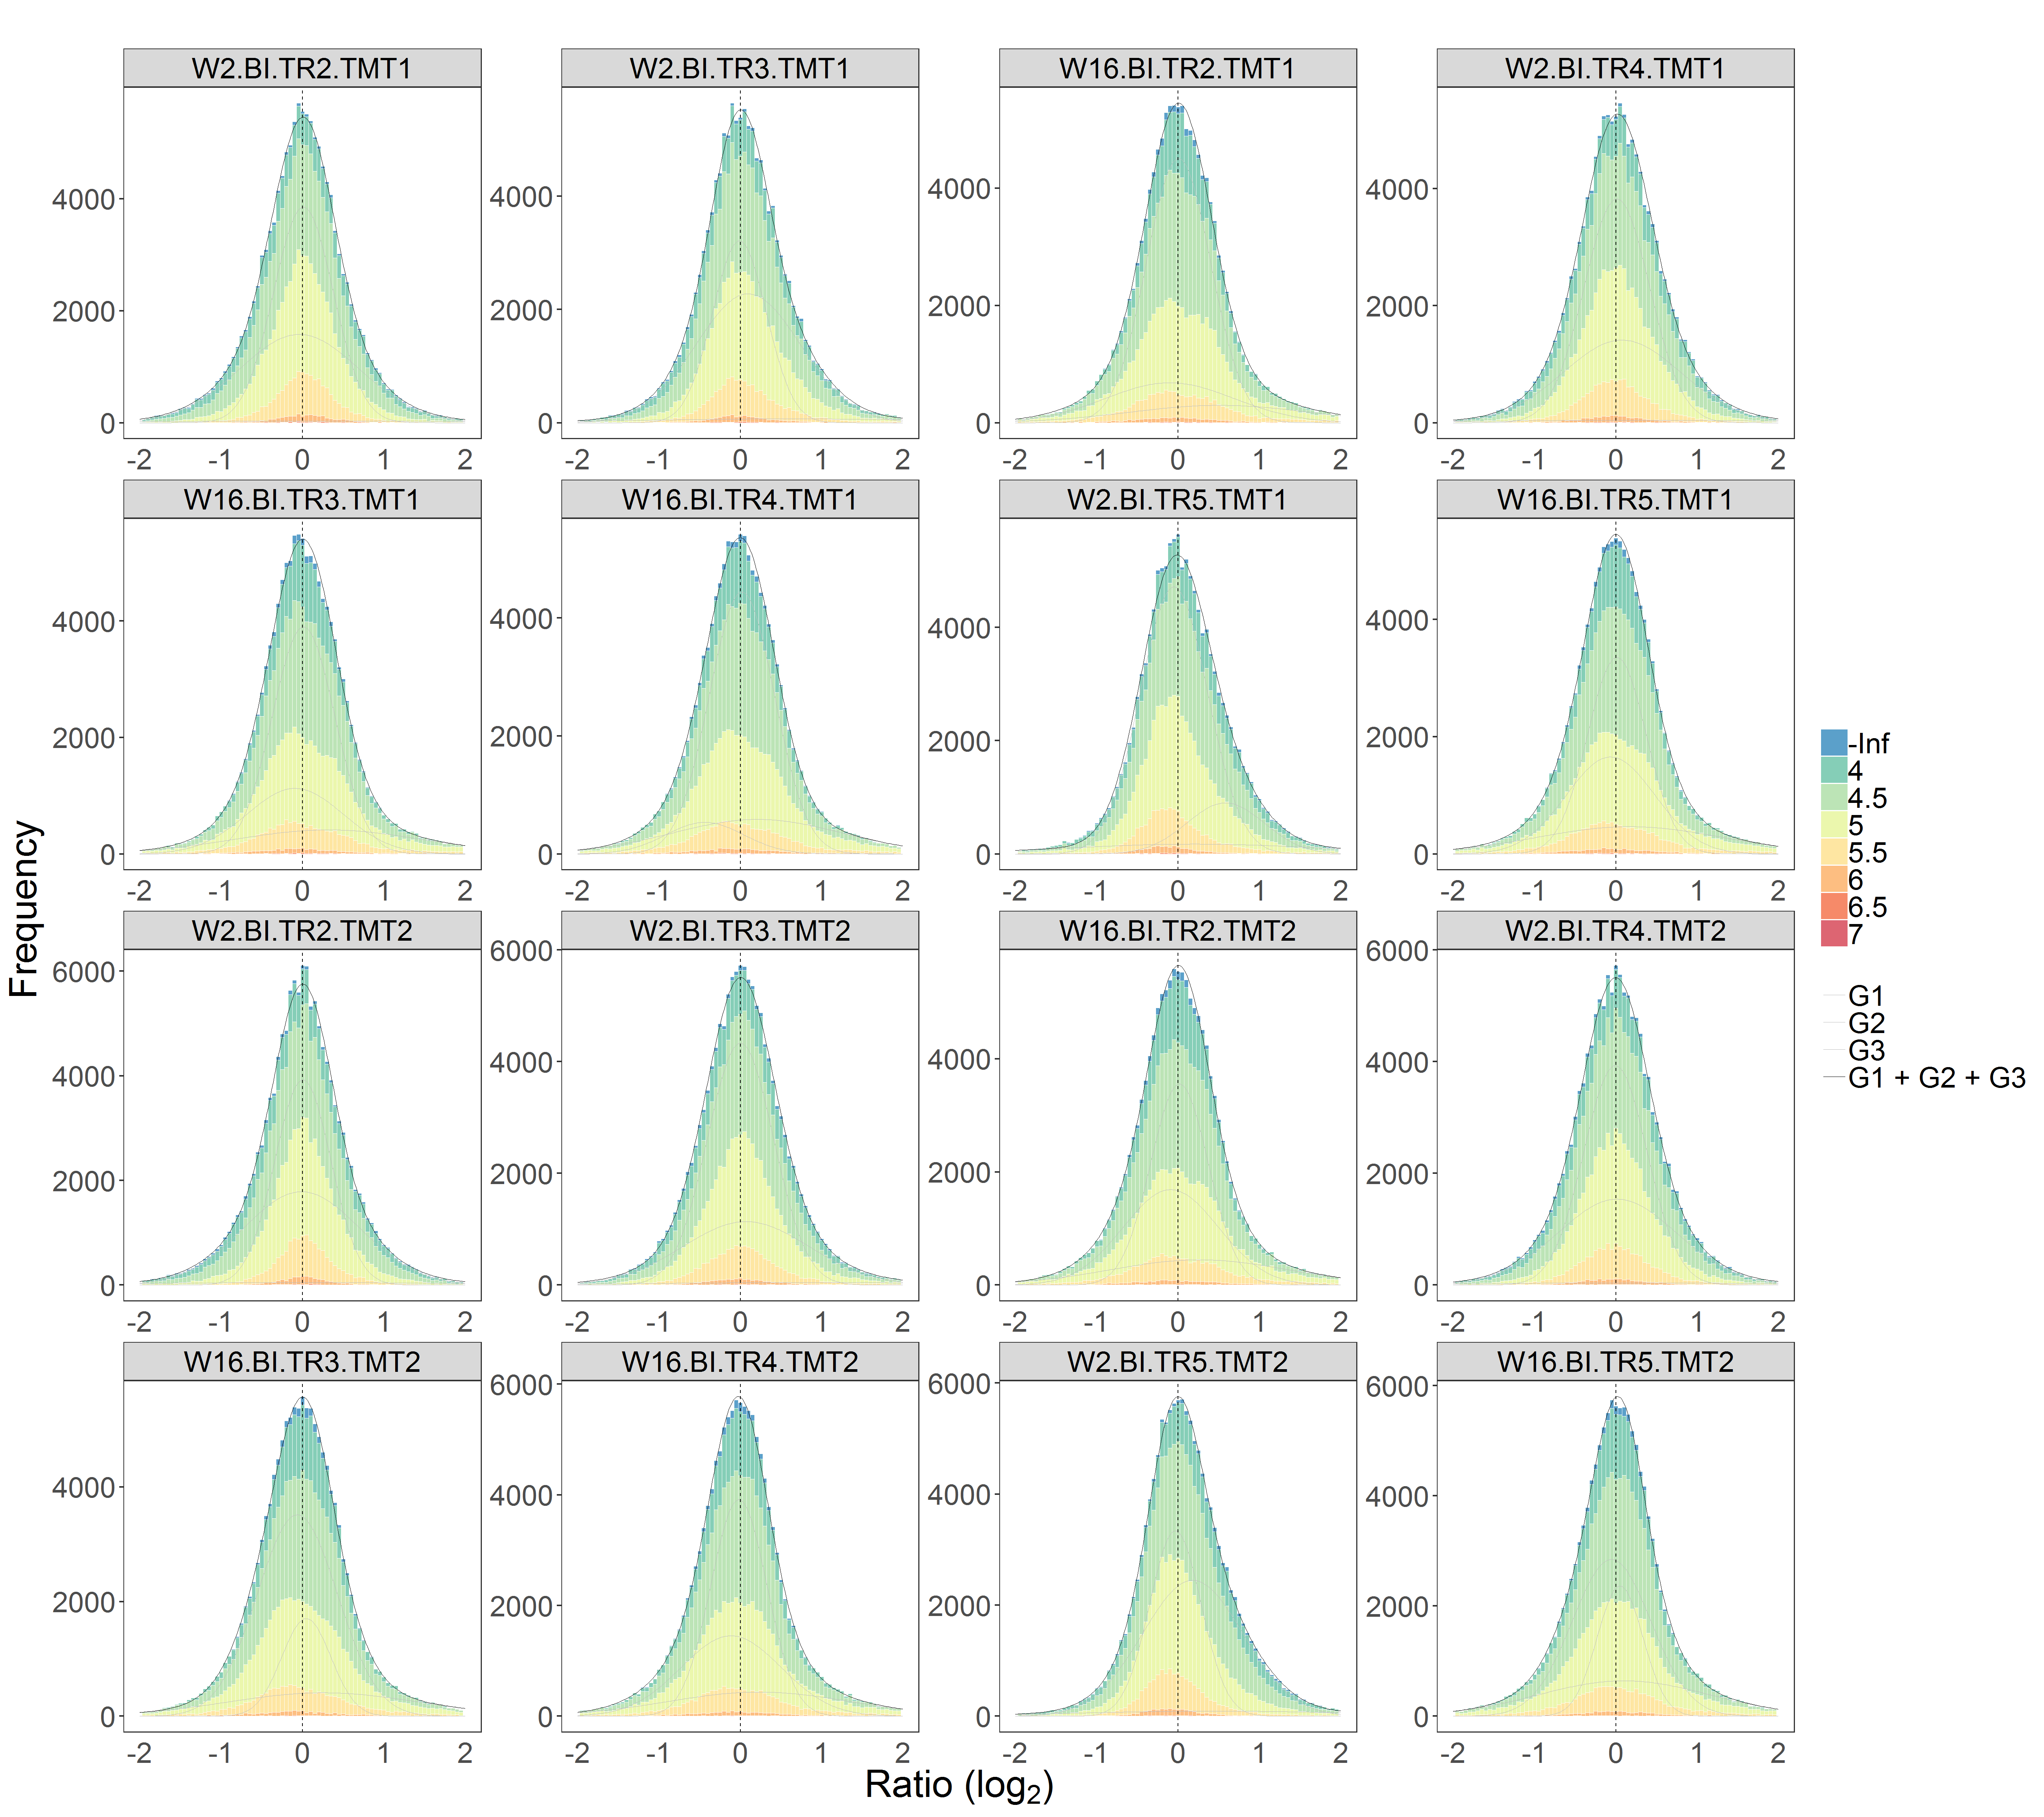
\includegraphics[width=0.45\linewidth]{images\peptide\histogram\bi_cmbn_peptides} 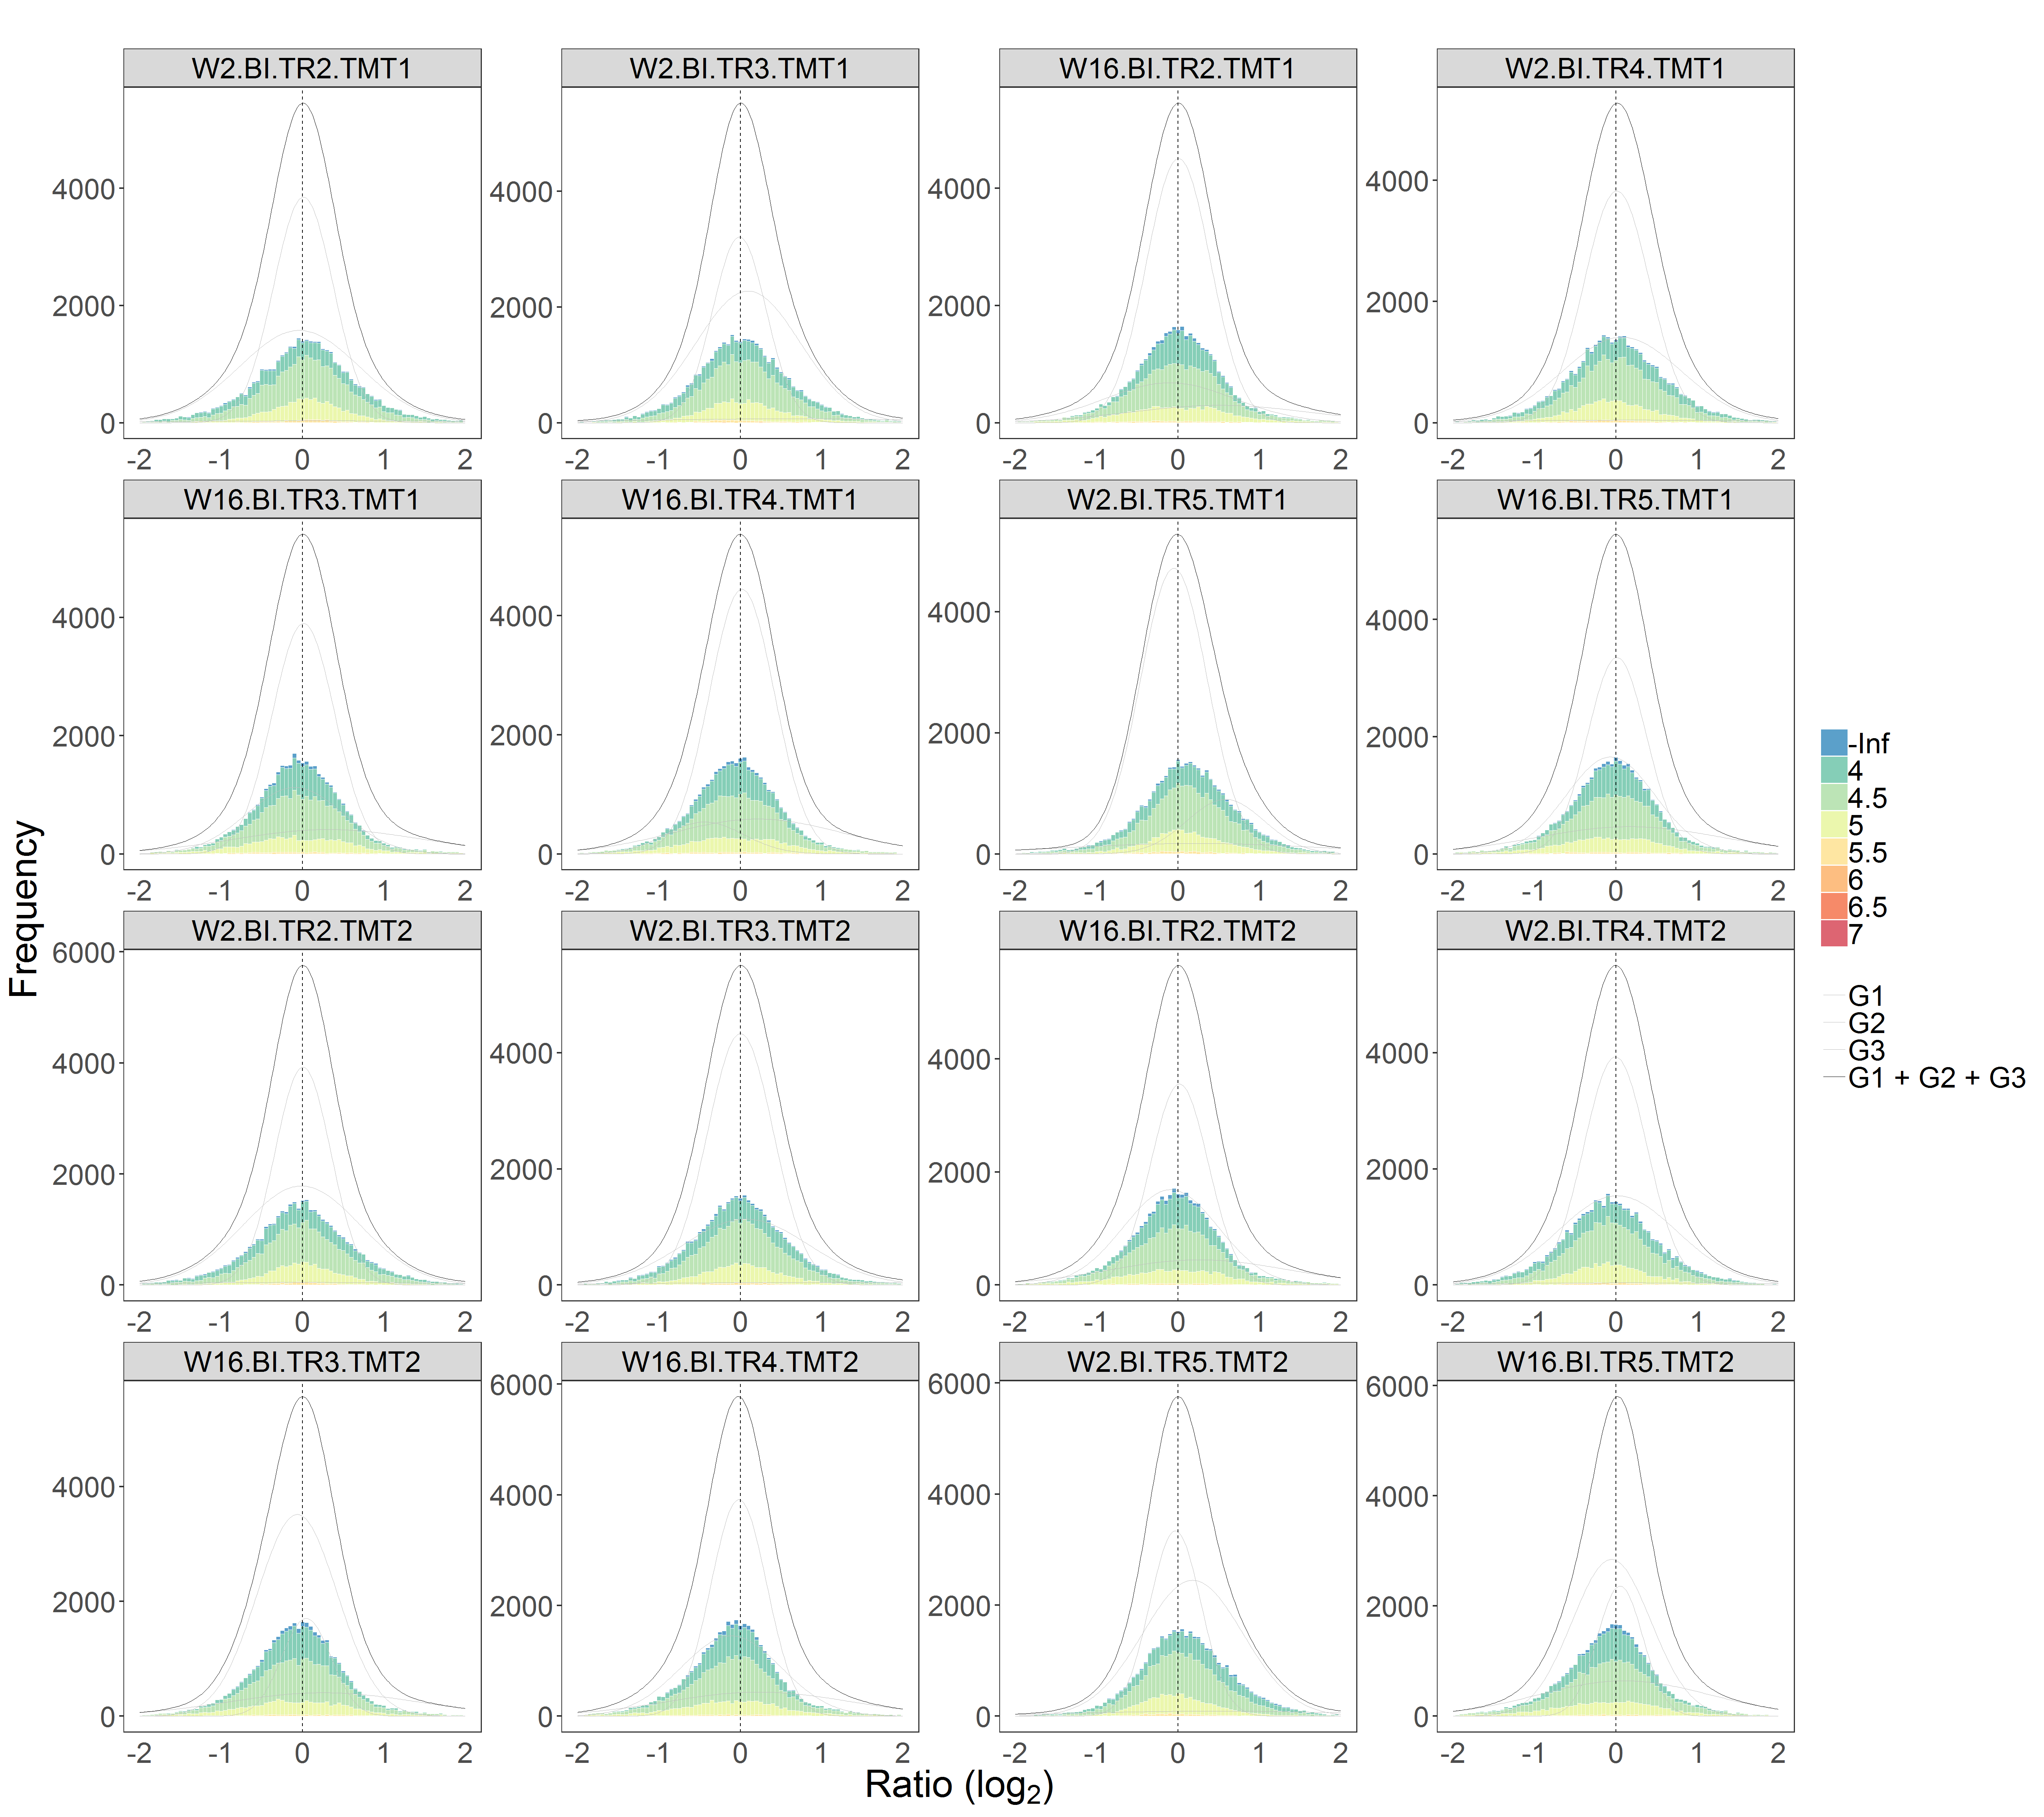
\includegraphics[width=0.45\linewidth]{images\peptide\histogram\bi_phospho_sub} \hfill{}

\caption{**Figure S2A-S2B.** Histogram visualization of peptide log2FC. Left: global + phospho; right: phospho only.}\label{fig:peptide_subset_hist}
\end{figure}

\hypertarget{references}{%
\subsubsection*{References}\label{references}}
\addcontentsline{toc}{subsubsection}{References}

\hypertarget{refs}{}
\leavevmode\hypertarget{ref-mertins2018np}{}%
Philipp, Martins. 2018. ``Reproducible Workflow for Multiplexed
Deep-Scale Proteome and Phosphoproteome Analysis of Tumor Tissues by
Liquid Chromatography-Mass Spectrometry.'' \emph{Nature Protocols} 13
(7): 1632--61. \url{https://doi.org/10.1038/s41596-018-0006-9}.

\leavevmode\hypertarget{ref-wangyy2011proteomics}{}%
Wang, Y. 2011. ``Reversed-Phase Chromatography with Multiple Fraction
Concatenation Strategy for Proteome Profiling of Human MCF10A Cells.''
\emph{Proteomics.} 11 (10): 2019--26.
\url{https://doi.org/10.1002/pmic.201000722}.


\end{document}
